\emph{{\bfseries Экономика, бизнес и услуги}}

{\bfseries Джангельдина Д.И., Рустемова С.М., Абеуханова Е.Б., Омарова
К.А., Ахметова Г.Б.}

\emph{ТУРИСТІК-РЕКРЕАЦИЯЛЫҚ АЙМАҚТАРДЫ БАСҚАРУ, ҚҰРУ ЖӘНЕ ДАМЫТУДАҒЫ
ТЕОРИЯЛЫҚ ӘДІСТЕМЕЛІК
НЕГІЗДЕРІ...............................................................................}

{\bfseries Батцэнгэл Х.}

\emph{ЭКОНОМИКА В «ДУХОВНОМ ИЗМЕРЕНИИ» И НОВАЯ «БИЗНЕС
МОДЕЛЬ»\ldots\ldots\ldots\ldots.}

{\bfseries Ж. Бидахмет, А.Р. Исаев}

\emph{КҮРДЕЛІ БИЗНЕС ПРОЦЕСТІ БАСҚАРУДЫҢ АҚПАРАТТЫҚ ЖҮЙЕСІ МЕН АЙМАҚТЫҚ
ДАМУДЫҢ КӨП НҰСҚАЛЫ РЕГРЕССИЯЛЫҚ
ТАЛДАУЫ.......................................................}

{\bfseries Садвокасова К.Ж., Бактымбет А.С., Садвокасов Р.К., Алпысбаева
А.К., Рейдолда С.}

\emph{ДЕНЕЖНАЯ СИСТЕМА НЕЗАВИСИМОГО КАЗАХСТАНА: СТАНОВЛЕНИЕ И
НАПРАВЛЕНИЯ ДАЛЬНЕЙШЕГО
РАЗВИТИЯ\ldots\ldots\ldots\ldots\ldots\ldots\ldots\ldots\ldots\ldots\ldots\ldots\ldots\ldots\ldots\ldots\ldots\ldots\ldots\ldots\ldots\ldots\ldots\ldots\ldots\ldots\ldots\ldots\ldots\ldots\ldots\ldots{}}

{\bfseries Serikkyzy A., Akhmetova A.B., Zhamalidenov S.E.}

\emph{APPROACHES TO MEASURING THE CREATIVE ECONOMY AND TRENDS IN THE
DEVELOPMENT OF THE IT SECTOR: THE IMPACT OF DIGITAL TECHNOLOGIES ON
CREATIVE
INDUSTRIES\ldots\ldots\ldots\ldots\ldots\ldots\ldots\ldots\ldots\ldots\ldots\ldots\ldots\ldots\ldots\ldots\ldots\ldots\ldots\ldots\ldots\ldots\ldots\ldots\ldots\ldots\ldots\ldots\ldots\ldots\ldots\ldots\ldots\ldots\ldots\ldots\ldots\ldots\ldots\ldots{}}

\emph{{\bfseries Экономика, бизнес и услуги}}\newpage
{\bfseries ҒТАМР 71.37.75}

{\bfseries ТУРИСТІК-РЕКРЕАЦИЯЛЫҚ АЙМАҚТАРДЫ БАСҚАРУ, ҚҰРУ ЖӘНЕ ДАМЫТУДАҒЫ
ТЕОРИЯЛЫҚ ӘДІСТЕМЕЛІК НЕГІЗДЕРІ}

{\bfseries Д.И. Джангельдина, С.М. Рустемова, Е.Б. Абеуханова, К.А.
Омарова, Г.Б. Ахметова}

Қ.Құлажанов атындағы Қазақ технология және бизнес университеті, Астана,
Қазақстан,

Корреспондент-авто: dariga\_da@mail.ru

Мақалада рекреациялық аймақтардағы туризмді қалыптастырудың теориялық
және әдістемелік негіздері қарастырылады. Туризм және рекреациялық
индустрияның облыстың әлеуметтік-экономикалық жүйесіне терең
интеграциясы, туризм мен рекреацияның, аумақтың әлеуметтік-экономикалық
дамуын басқарудың жалпы стратегиясы мен бағдарламасының басқару
мүмкіндігі көрсетілген. Аймақтың туристік-рекреациялық әлеуеті
тұжырымдамасы жүйелік көзқарас тұрғысынан тұжырымдалған. Ең алдымен
аймақтың туристік-рекреациялық мамандануын құрайтын табиғи ресурстар
қарастырылады, рекреациялық және туристік әлеует дәрежесіне қарай
туристік-рекреациялық сфераның негізгі құрамдас бөлігі ретінде табиғи
ресурстардың классификациясы әзірленді. Авторлар экономикалық бағалау
үшін табиғи рекреациялық ресурстарды пайдалану мүмкіндіктерін анықтау
қажеттілігіне назар аударады, осыған байланысты тікелей және жанама
рекреациялық ресурстар қарастырылады. Экономиканың туристік-рекреациялық
секторының пайда болуы мен дамуының маңызды шарты туристік және
рекреациялық ресурстар мен қызметтерге сұраныс, сондай-ақ аймақтың
қолжетімділігі мен дамуы болып табылатыны көрсетілген, оны негізінен
мемлекет анықтайды. Аумақтардың ресурстық әлеуетін бағалаудың келесі
бағыттары ұсынылады: ресурстарды сандық бағалау, әлеует құрылымын
бағалау, жеке потенциалды пайдалану дәрежесі, ресурстарды пайдалану
мүмкіндіктерін бағалау; туристік-рекреациялық кадастрлар жүйесін енгізу.
Туристік-рекреациялық ресурстарды бағалау әдістері мен рейтингтік шкала
параметрлері берілген.

{\bfseries Түйін сөздер:} туризм, рекреация, аумақтық-рекреациялық жүйе,
рекреациялық ресурстар, табиғи ресурстар, туристік ресурстар кадастры.

{\bfseries ТЕОРЕТИЧЕСКИЕ МЕТОДОЛОГИЧЕСКИЕ ОСНОВЫ УПРАВЛЕНИЯ, СТРОИТЕЛЬСТВА
И РАЗВИТИЯ ТУРИСТО-РЕКРЕАЦИОННЫХ РЕГИОНОВ}

{\bfseries Д.И. Джангельдина\textsuperscript{,}, С.М. Рустемова, Е.Б.}
{\bfseries Абеуханова, К.А. Омарова, Г.Б. Ахметова}

\textsuperscript{1}Казахский университет технологии и бизнеса имени
К.Кулажанова, Астана, Казахстан,

e-mail: dariga\_da@mail.ru

В статье рассматриваются теоретические и методологические основы для
формирования туризма в рекреационных регионах. Показана глубокая
интегрированность индустрии туризма и рекреации в
социально-экономическую систему региона и обоснована отсутствие
возможности для управления развитием туризма и рекреации отдельно от
общей стратегии и программы управления социально-экономическим развитием
территории. Понятие туристско-рекреационного потенциала региона
формулируется с позиции системного подхода. Рассматриваются природные
ресурсы, которые, в первую очередь, формируют туристско-рекреационную
специализацию региона, разработана классификация природных ресурсов как
основного компонента туристско-рекреационной сферы, по степени
рекреационного и туристского потенциала. Авторы обращают внимание на
необходимость определения возможностей использования природных
рекреационных ресурсов для экономической оценки, в связи с этим
рассмотрены прямые и опосредованные рекреационные ресурсы. Показано, что
важным условием возникновения и развития туристско-рекреационного
сектора экономики является востребованность туристско-рекреационных
ресурсов и услуг, а также доступность и освоенность региона, что в
значительной степени определяется состоянием туристско-рекреационной
инфраструктуры. Предложены такие направления оценки ресурсного
потенциала территорий как количественная оценка ресурсов, оценка
структуры потенциала, степень использования частных потенциалов, оценка
возможностей использования ресурсов; введение системы
туристско-рекреационных кадастров. Приведены методики оценки
туристско-рекреационных ресурсов, параметры оценочных шкал.

{\bfseries Ключевые слова}: туризм, рекреация, территориально-рекреационная
система, рекреационные ресурсы, природные ресурсы, кадастр туристских
ресурсов.

{\bfseries THEORETICAL METHODOLOGICAL FOUNDATIONS OF ADMINISTRATION,
CONSTRUCTION AND DEVELOPMENT OF TOURIST-RECREATION AREAS}

{\bfseries D.I. Dzhangeldina, S.M. Rustemova, E.B. Abeukhanova, K.A.
Omarova, G.B. Akhmetova}

К.Kulazhanov Kazakh University of Technology and Business, Astana,
Kazakhstan,

e-mail: dariga\_da@mail.ru

The article discusses the theoretical and methodological foundations for
the formation of tourism in recreational regions. The deep integration
of the tourism and recreation industry into the socio-economic system of
the region is shown and the lack of opportunity to manage the
development of tourism and recreation separately from the general
strategy and program for managing the socio-economic development of the
territory is substantiated. The concept of tourism and recreational
potential of the region is formulated from the perspective of a systems
approach. Natural resources are considered, which, first of all, form
the tourism and recreational specialization of the region, a
classification of natural resources as the main component of the tourism
and recreational sphere has been developed, according to the degree of
recreational and tourism potential. The authors draw attention to the
need to determine the possibilities of using natural recreational
resources for economic assessment; in this regard, direct and indirect
recreational resources are considered. It is shown that an important
condition for the emergence and development of the tourism and
recreational sector of the economy is the demand for tourism and
recreational resources and services, as well as the accessibility and
development of the region, which is largely determined by the state of
the tourism and recreational infrastructure. The following directions
for assessing the resource potential of territories are proposed:
quantitative assessment of resources, assessment of the structure of
potential, the degree of use of private potentials, assessment of the
possibilities of using resources; introduction of a system of tourist
and recreational cadastres. Methods for assessing tourist and
recreational resources and parameters of rating scales are presented.

{\bfseries Keywords}: tourism, recreation, territorial and recreational
system, recreational resources, natural resources, cadastre of tourist
resources.

{\bfseries Кіріспе.} Қазіргі заманғы туризм күрделі әлеуметтік-экономикалық
және кеңістіктік құбылыс ретінде, халық шаруашылығының күрделі саласы
ретінде, әлеуметтік-экономикалық дамудың катализаторы болып табылады
және табиғи ресурстарды экологиялық тұрғыдан тиімді пайдалану негізінде
адамдардың жоғары өмір сүру сапасын қамтамасыз ету өзекті мәселердің
бірі болып саналады.

Туристік-рекреациялық аймақтарды басқару, құру және дамытудағы теориялық
әдістемелік тәсілдерді зерттеуде «туристік-рекреациялық ресурстар» мен
«рекреациялық аудандар» және оларды қалыптастыру факторларының түрлерін
анықтау зерттеудің басты мақсаты болып табылады.

Зерттеу обьектісі - Туристік-рекреациялық аймақтарды басқару, құру және
дамыту мәселесі мен қалыптасу кезеңдері.

Зерттеу пәні: Туристік рекреациялық қызметі мен рекреациялық -- туристік
аймақтарды дамыту ерекшеліктері және аумақтық ұйымдастыру болып
табылады.

Зерттеу әдістері. Зерттеудің әдіснамалық негізі жалпы ғылыми
диалектикалық, жүйелік, сонымен қатар экономикалық -- математикалық
модельдеу әдістері, экономикалық талдау мен синтез, эмпирикалық жалпылау
және т.б.

Рекреациялық аудандастыру табиғи негізге негізделген. Дегенмен, табиғи
база айтарлықтай артық, рекреациялық аймақтардың мүмкіндіктері мен
қажеттіліктері өте шектеулі. Бұл қайшылықтың нәтижесі рекреациялық даму
үшін нақты аумақты таңдау көбінесе аумақтың әлеуметтік-мәдени дамуының
қажеттіліктерімен анықталады. Әртүрлі аймақтардың арасында рекреациялық
дамуға үміткерлер олардың дамуының нақты мүмкіндіктеріне қарағанда
әлдеқайда көп.

Бұл рекреациялық мақсаттағы аумақты игерудің бастапқы кезеңдеріне де,
рекреациялық дамудың қол жеткізілген деңгейін сақтау кезеңіне де
қатысты. Аймақтарды бөлу процедурасын бөлек қарастыруға болмайды,
өйткені бұл мамандардың тек зияткерлік күш-жігерінің нәтижесі емес - бұл
шындықтың көрінісі. Бірінші орында, әрине, нақты кеңістікте жүріп жатқан
процесс. Ол аймақтарды өздері жасайды, содан кейін оларды сәйкестендіру
стандарттарын белгілейді. Аймақтарды бөлу процедурасы тек қатаң
белгіленген критерийлерге сәйкес аудандарды ойлау болып табылады.
Аймақтандырудағы өзгерістер ғылыми аймақтандыру саласындағы табиғи және
сәйкес өзгерістерге, оның ішінде ғылыми рәсім ретінде аймақтандыруды
дамытуды ынталандыруға әкеп соғады; объект тұрақты болып табылады және
онда тек сандық емес, сонымен қатар сапалық өзгерістер болады.

Туристік ресурс пен маркетингтік зерттеулердің ерекшеліктеріне сүйене
отырып, әртүрлі дәрежедегі аумақтық туристік кешендердің түрлері мен
өлшемдерінің оңтайлы арақатынасы анықталады; орналастыру үшін ең қолайлы
туристік кәсіпорындарды таңдау негізделген; осы аумақтардың рекреациялық
мүмкіндіктері және жаңадан құру және бұрыннан құрылған туристік
аймақтардың рекреациялық әлеуетін арттыру үшін қажетті күрделі
салымдардың көлемі есептеледі. Туристік аудандастыру аумақтың барлық
бөліктеріндегі туризмнің жай-күйі, даму факторлары мен перспективалары
туралы тұтас көрініс алуға, оларды бір-бірімен салыстыруға және бұл
ақпаратты туризмді жоспарлау мен басқаруда пайдалануға мүмкіндік береді.

Рекреациялық аймақтардың дамуына көптеген факторлар айтарлықтай әсер
етеді, мысалы: аумақтың экономикалық даму деңгейі; аймақ шегінде
аумақтың көліктік қолжетімділігі; жеткілікті еңбек ресурстарының болуы;
есеп айырысу жүйесінің болуы. Бұл рекреациялық аймақты дамытудың нақты
процесінің нақты факторлары. Екінші жағынан, олардың жоқтығы соншалықты
маңызды рөл атқармайды және белгілі бір аумақты рекреациялық аймақ
ретінде дамыту міндетін алып тастамайды. Бұл процесте ең бастысы бір
аумақты игеру қажеттілігі және егер ол рекреациялық аймақ ретінде
игерілсе, онда жоғарыда аталған факторлардың қаншалықты қолайлы
болғанына қарамастан мәселелер шешіледі.

Аймақтық қалыптасудың алғашқы себебі -- белгілі бір аумақтың
әлеуметтік-мәдени дамуының қажеттілігі. Оны дамытудың нақты бағытын
таңдау аумақтың әлеуеті мен ерекшеліктеріне байланысты. Бұл өнеркәсіптік
даму, рекреациялық немесе кез келген басқа болуы мүмкін. Жасалған
таңдауға байланысты рекреациялық, өндірістік немесе басқа аумақты
қалыптастыру процесі басталады. Олардың қай-қайсысы да белгілі аумақты
игерудің жалпы процесінің салдары, белгілі бір түрі ғана болып табылады

Рекреациялық аудандастыру табиғи негізге негізделген. Дегенмен, табиғи
база айтарлықтай артық, рекреациялық аймақтардың мүмкіндіктері мен
қажеттіліктері өте шектеулі. Бұл қайшылықтың нәтижесі рекреациялық даму
үшін нақты аумақты таңдау көбінесе аумақтың әлеуметтік-мәдени дамуының
қажеттіліктерімен анықталады. Әртүрлі аймақтардың арасында рекреациялық
дамуға үміткерлер олардың дамуының нақты мүмкіндіктеріне қарағанда
әлдеқайда көп.

Бұл рекреациялық мақсаттағы аумақты игерудің бастапқы кезеңдеріне де,
рекреациялық дамудың қол жеткізілген деңгейін сақтау кезеңіне де
қатысты. Аймақ халқының жыл сайынғы рекреациялық қызметі өте шектеулі
ресурс болып табылады, сондықтан ол осы әлеуметтік-мәдени жүйенің
қажеттіліктеріне байланысты қайта бөлінеді. Көптеген жолдармен
аумақтардың рекреациялық даму процесі, тіпті шын мәнінде бірегей
сипаттамаларымен анықталады.

Туристік қызмет және туристік ресурстар, туристік іс-әрекет, турист -
туристік қызметті тұтынушы ретінде қалыптасады . Туристік қызмет түрі
ретінде жұмыс істеуге туристік өнім, туристік тауарлар, туристік және
туристік маршрут, туристік қызметтерді стандарттау және сертификаттау,
туризмнің түрлері мен жіктелуі, белсенді және пассивті туризм, турлардың
түрлері, арнайы турлар сияқты мәселелерді ашып қарастырады. Аумақтық
географиялық жүйе ретінде бір-бірімен тығыз байланыстағы жүйе асты
құрылымдар: табиғи, мәдени кешендер, инженерлік құрылымдар, қызмет
көрсетушілер тобы, басқарушылар мен демалушыларды қамту қажеттілігіне
назар аударады. Туристік іс-әрекеттер мен шаралар адамзат әрекеті
барысында адам-қоғам өміріндегі өте қажетті көпсалалы пайда болған
құбылыс. Қазіргі кезде туристік қызмет және туристік іс-әрекет деген екі
ұғым жиі қолданыста кездеседі. Олар туризм индустриясы мен туризм
салаларының басты көрсеткіші болып саналады. Туризм «кеңістік әлеуметтік
- экономикалық құбылыс» дей отырып оның аумақта пайда болуы негіз
саналады. Шетелдік туризмге қатысты басылымдарда экономика ғылымы
туризмді күрделі экономикалық әлеуметтік жүйе ретінде қарастырады.
Олардың туризм индустриясын басты компонент деп санаулары орынды
{[}1{]}. Біз қарастырған зерттеулер қазіргі туризмді көпқырлы, көпсалалы
құбылыс деп, экономикалық, жаратылыстану, қоғамдық, гуманитарлық т.б.
ғылым салаларымен байланыстырып, кешенді тұрғыда терең зерттеу
керектігін көрсетеді. Туризмнің ғылым ретінде қалыптасып дамуына Рессей
ғалымдары В.С. Преображенский, Ю.А. Веденин, В. Даринский, А.
Александрова т.б. зерттеулері мен еңбектерін атап өткен жөн {[}2{]}.
География ғылымы тарапынан Қазақстандық профессор С.Р. Ердаулетов және
оның шәкірттері, нақты айтсақ Аль-Фараби атындағы Қазақ Ұлттық
университеті ғалымдары атсалысуда. Әдебиеттермен ғылыми мақалаларға
талдау беру барысында туризм ғылымы салаларының ел экономикасының
дамуына қосар үлесі зор екендігін түсінуге болады. Олардың қатарында А.
Ахтымбаева, Ш. Абдреева, Ж.Н. Алиева т.б. бар. Әр түрлі деңгейдегі
әлеуметтік-экономикалық жүйелердің әртүрлі формалары, сондай-ақ олардың
жеке ішкі жүйелері ішінара қарастырылуда.

{\bfseries Материалдар мен әдістер.} Аудандастыру -- аймақтық қалыптасу
процесін зерттеумен байланысты ғылыми процедура. Аймақтарға бөлу қатаң
теория мен әдістемеге негізделген (немесе, кем дегенде, оны негіздеген
жөн). Рекреациялық аудандастыру -- іргелі негізде адекватты сипаттауға
болатын бір ғана аспектіні (рекреацияны) көрсететін жеке, салалық
аудандастыру түрі. Рекреациялық мақсаттағы жекелеген аумақтарды дамыту
аймақ кеңістігін қалыптастырудың жалпы процесінің қарапайым бөлігі болып
табылады. Рекреациялық аймақтың қалыптасу және оның аудандастыру
процестерін дұрыс түсінудің негізі аумақтардың әлеуметтік-мәдени даму
процестерінің сәйкес адекватты сипаттамасы болып табылады.

Аймақтарды бөлу процедурасын бөлек қарастыруға болмайды, өйткені бұл
мамандардың тек зияткерлік күш-жігерінің нәтижесі емес - бұл шындықтың
көрінісі. Бірінші орында, әрине, нақты кеңістікте жүріп жатқан процесс.
Ол аймақтарды өздері жасайды, содан кейін оларды сәйкестендіру
стандарттарын белгілейді. Аймақтарды бөлу процедурасы тек қатаң
белгіленген критерийлерге сәйкес аудандарды ойлау болып табылады.
Аймақтандырудағы өзгерістер ғылыми аймақтандыру саласындағы табиғи және
сәйкес өзгерістерге, оның ішінде ғылыми рәсім ретінде аймақтандыруды
дамытуды ынталандыруға әкеп соғады; объект тұрақты болып табылады және
онда тек сандық емес, сонымен қатар сапалық өзгерістер болады.

Рекреациялық аудандастыру маңызды ғылыми және практикалық процедура
болып табылады. Бұл рекреациялық қызмет географиясы мен рекреациялық
қызмет көрсету секторында көп нәрсені түсінуге мүмкіндік беретін тиімді
және өте қажет ғылыми әдіс. Бұл тәжірибе үшін өте пайдалы болды және оны
негізінен ірі мемлекеттік ұйымдар пайдаланды. ТМД елдерінің жаңа
шындықтары жағдайында рекреациялық аудандастыру айтарлықтай өзгеруде
және тек үлкен емес, сонымен қатар орта және тіпті шағын басқару
шешімдерін қабылдау құралына айналуда: рекреациялық аудандастыру және
рекреациялық нарықтағы тенденцияларды білу негізінде, ол жекелеген
туристік компаниялар мен банктер деңгейінде инвестицияны тиімді
жоспарлауға және жүзеге асыруға болады {[}3{]}.

Туристік ресурс және оны аймақтық деңгейде пайдалану - ландшафттардың,
климаттың, флора мен фаунаның және басқа да туристік ресурстардың
әртүрлілігі туризм туралы географиялық және экономикалық ақпаратты
жүйелеу және оның дамуының аумақтық заңдылықтарын анықтау үшін әртүрлі
аймақтарды анықтау қажеттілігіне әкеледі.

Туристік ресурс пен маркетингтік зерттеулердің ерекшеліктеріне сүйене
отырып, әртүрлі дәрежедегі аумақтық туристік кешендердің түрлері мен
өлшемдерінің оңтайлы арақатынасы анықталады; орналастыру үшін ең қолайлы
туристік кәсіпорындарды таңдау негізделген; осы аумақтардың рекреациялық
мүмкіндіктері және жаңадан құру және бұрыннан құрылған туристік
аймақтардың рекреациялық әлеуетін арттыру үшін қажетті күрделі
салымдардың көлемі есептеледі.

Туристік аудандастыру аумақтың барлық бөліктеріндегі туризмнің жай-күйі,
даму факторлары мен перспективалары туралы тұтас көрініс алуға, оларды
бір-бірімен салыстыруға және бұл ақпаратты туризмді жоспарлау мен
басқаруда пайдалануға мүмкіндік береді.

Экономиканы жаңғырту процестері жүріп жатқан елдерде туризм мен
рекреацияның дамуының негізгі тенденциялары мен перспективаларын анықтау
әртүрлі факторлар мен жағдайлармен байланысты мәселелерді шешуге кешенді
көзқарасты талап етеді. Демек, жеке аймақта туризм және рекреациялық
сектордың қызмет етуінің жалпы негізін ұсыну мәселесі туындайды {[}4{]}.

Туризм сферасының дамуының кеңістікте орналасуының теориялық әдістемелік
негіздері бір-бірімен тығыз байланысты «туризм», «тұрақты даму»,
«тұрақты туризм» ұғымдарының пайда болуы мен дамуы теориялық тұрғыда
талданды. Туризмді тұрақты дамытудың критерийлері, сондай-ақ негізгі
қағидаттары қазіргі заманғы тұрақты туризмнің теориялық ұғымдарын
зерттеу барысында қарастырылды. Сонымен қатар, «аумақ» түсінігі мен
«кеңістік», «тұрақты даму» мен «туризм» ұғымдарының байланыстары
ғалымдардың еңбектерін талдау негізінде орнатылды. Жүргізілген әдеби
шолу шетелдік және отандық авторларды талдау негізінде «туризмнің
тұрақты дамуы» жалпы ұғымын ауқымы, мәні мен мазмұны нақтыланды. Жаңа
аумақтық рекреациялық құрылымды қарастырғанда қандай нақтылы бағытта
зерттеулер жүргізу керектігі айқындалды. Туристік зерттеулердегі
аумақтық рекреациялық жүйелерді зерттеудегі заманауи теориялары мен
әдістерінің маңызды міндеттері -- аумақтық туризмді ұйымдастыру схемасы
құрастырылды. Н.Ф. Реймерс тек рекреациялық ресурстар деп - табиғи және
мәдени ресурстар жиынтығы ретінде қарастырады. Ал Л.А. Багрова
анықтамасында «рекреациялық-ресурстар» - бұл табиғи, табиғи-техникалық
және әлеуметтік-экономикалық геожүйелер және материалдық мүмкіндіктер
деп берілген. Сонымен, 1-кестеде Н.Ф. Реймерс бойынша
рекреациялық-туристік ресурстар көп салалы жан жақты ресурстарды
жіктегенде қолданбалы жағын қарастырған {[}4{]}.

{\bfseries 1 --Кесте -Туристік-рекреaциялық ресурстар типтері}

\begin{figure}[H]
	\centering
	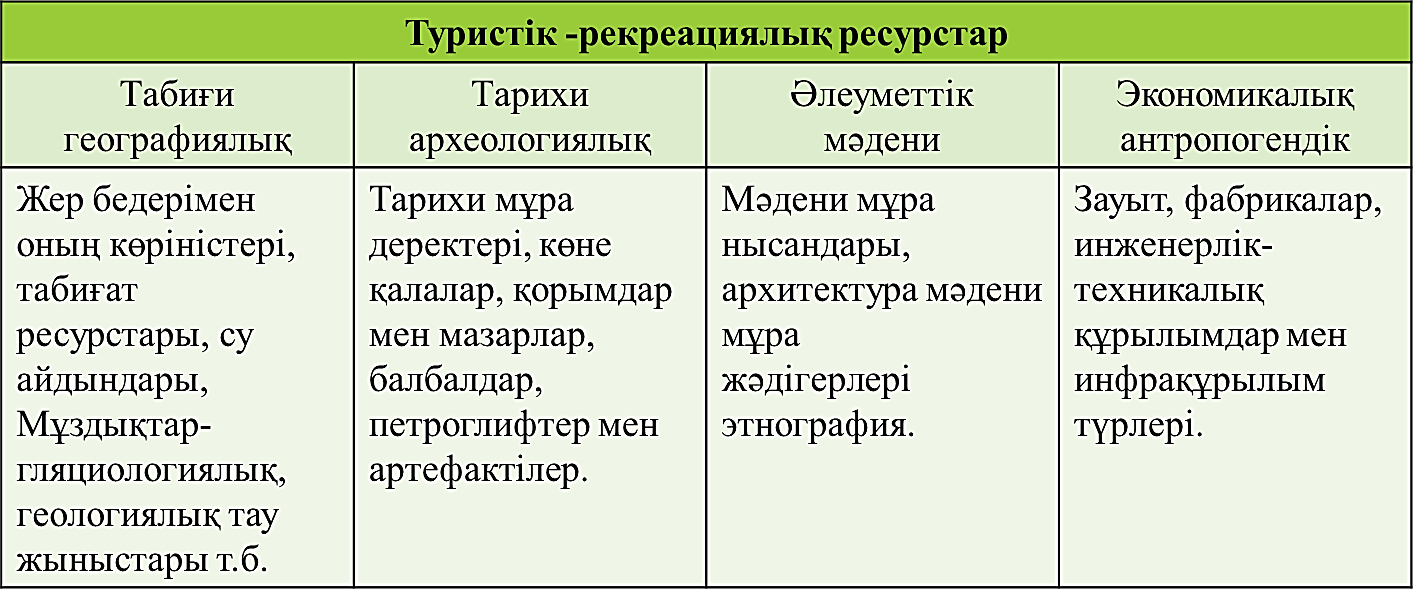
\includegraphics[width=0.8\textwidth]{assets/1110}
	\caption*{}
\end{figure}

\emph{{\bfseries Примечание -Дерек көздері негізінде құрастырылған
{[}4{]}}}

Жеке аумақтардың рекреациялық туристік мүмкіндіктерін бағалауда алдымен
нысандар тізілімі жасалып ресурстық әлеует анықталады. Олардың екіге
бөліп, антропогенді және табиғи ресурстар тобы деп қарастырылады.

Жеке өңірлер де туризмді дамытудың теориялық әдіснамалық астары аумақтық
рекреациялық әлеуетті бағалауға қатысты болып келеді.

Аумақтық рекреациялық әлеуетті бағалау рекреациялық ресурстарды бағалау
теориясына бағынады. Ол географиялық ресурстарды тану сферасына жатады.
Географиялық бағалауларда жеке табиғат түрлерін бағалау бағыттарында
табиғат жағдайларын бағалау жолдары қарастырылады.

Табиғат ресурстарын, табиғи орта өзгерісін, адамдардың табиғи ортада
өмір сүру деңгейін сапалы бағалауа Е.А. Котлярова, Ю.Д. Дмитриевский,
A.A. Минц, Л.И. Мухина, B.C. Преображенский, т.б. ғалымдар өз үлестерін
айтарлықтай қосты.

Қазақстандық зерттеушілер физикалық географиялық тұрғыда бағалау жолдары
арқылы жекелеген әдіснамалық мәселелер қарастырды. Олар С.Р. Ердавлетов,
В.И. Попов, Ж.Н. Алиева, О.Б. Мазбаев, Е.А. Тоқпанов, Б.К. Асубаев, М.А.
Шабельникова, М.Д. Мамадияров т.б.

Экономика ғылымдары саласы бойынша туризм мәселелері қазақстандық А.Ж.
Садуов, Г.М. Дуйсен, Р.А. Асанбаева, А.Ш. Нургалиева т.б., Г.К.Аскарова
зерттеу жұмыстарында қарастырылған {[}5{]}.

Халық шаруашылығы салалары жүйесіндегі және аумақтық еңбек бөлінісіндегі
туризмнің орны ерекше. Осыған байланысты көптеген елдерде халықтың
рекреациялық қызметтерге деген өсіп келе жатқан әлеуметтік
қажеттіліктері демалыс, рекреацияны қалыптастыруға дамытуға негіз болды.

Қазіргі географиялық және экономикалық ғылымда демалыс аймағының немесе
рекреациялық саланың шекараларын анықтау мәселесі бойынша бірыңғай
ұстаным жоқ. Зерттеу мақсаттарына байланысты әртүрлі әдіснамалық
тәсілдер қолданылуда және пікірлер қалыптасуда.

Рекреациялық, қызмет көрсету саласы бойынша оның құрамындағы туризмді
көптеген зерттеушілер бөліп көрсетеді, бұл рекреациялық тұтынудың ең тез
дамып келе жатқан тармағы.

Шаруашылық кешеніндегі туристік саладағы іс әрекеттердің орнын анықталып
отырып, ол материалдық емес өндіріс салаларына жатқызылады. Өйткені ол
туристке қажетті туристік қызметтерді қалыптастырады. Туристік сұранысты
басшылыққа алатын салалардың өнімдері қызмет көрсету түрінде әрекет
ететіндіктен, мұндай қамту аясында қарастырылатын демалыс саласы
туристік қызмет болып табылады. Жұмыс күшін қалпына келтіруді және оның
сапасын арттыруды қамтамасыз ететін туристік сала материалдық өндірістің
жұмысына тікелей әсер етеді. Рекреациялық және туристік қызметтер тек
рекреациялық нысандар, ресурстар мен инфрақұрылымды ғана емес, толықтай
әлеуметтік-экономикалық байланыстар арқылы кешенді қалыптасқан кең
әлеуметтік-экономикалық кеңістікті де қамтиды.

Туристік іс-шаралардың негізі болып туристік ресурстар саналады.
Туристік қызметтерді тікелей қалыптастырушы туристік кәсіпорындар мен
туристік инфрақұрылым, олар бірге туристік экономиканы құрайды.
Қызметтерді өндіруші ретінде ол халықтың өмір сүру деңгейін жоғарылатуда
өте маңызды рөл атқарады. Халықтың өмір сүру үшін қажетті материалдық
және мәдени-рухани нысандармен қамтамасыз етілуі, оларды тұтыну
деңгейіне жету және адамдардың осы тауарларға деген қажеттіліктерін
қанағаттандыру дәрежесі болып табылады. Туристік экономика елдің
экономикалық кешеніне қарқынды түрде еніп, туристерге қызмет көрсетумен
тығыз байланысты материалдық және материалдық емес өндірістің әртүрлі
салаларымен байланысты толықтай «туризм индустриясын» құрайды.

Қазақстан егемендік алған жылдары экономикадағы туристік саланы дамыту
туралы бірнеше құжаттар қабылдап туристік нарықты дамыту бағытында
іс-шаралар жүргізіп келеді. Туризм индустриясы немесе шаруашылық саласы
ретінде қарастыруда соңғы жылдары ғалымдар арасында әртүрлі пікірлер
қалыптасты. География ғылымның алдына аймақтағы табиғи-ресурстық
әлеуетті қолданумен байланысты мәселені қарастырудың қажеттілігіне орай
зерттеулер жүргізіле бастады. Олар аумақтық, кеңістік тұрғысында «табиғи
рекреациялық ресурс» және «рекреациялық аймақ» деген ұғымдардың
қалыптасуына ықпалын тигізді.

Экономикалық зерттеулер туристік нарық, сұраныс пен ұсыныстарға қатысты,
көпшілік жағдайда қонақүй бизнесі мен мейрамхана ісіне байланысты
жүргізілуде. Туристік-рекреациялық іс-әрекеті ұйымдастыру мәселесі
кезінде салыстырмалы түрде тауарлар мен қызметтерді тұтыну нарығының
маңызды құрамдас бөлігі, туризмді қарқынды дамытудың
ұйымдастырушылық-экономикалық тетігі бағытында қарастырылуы болатын.
Барлық салада рекреациялық тақырыптар соңғы кездерде жиі көтеріліп отыр.

Рекреациялық деген ұғым адамдардың бос уақыты кезінде демалу, сауықтыру
мақсатындағы іс әрекеттері. Қазақстандық зерттеушілер С.Р. Ердаулетов
т.б. еңбектерінде бос уақыт, демалыс, туристік әрекеттер-рекреациялық
шаралар туралы айтылады. Ғылыми әдебиеттерге шолу барысында аумақтық
туризмді дамытуға байланысты осы мәселелерге басты назар аударылды.
Территорияны пайдаланумен байланысты шаруашылық қызметтің әртүрлі
түрлері, әртүрлі шаруашылық жерлерді қажет ететіні сияқты, рекреация
үшін де әртүрлі жерлер қажет (серуендеуге, жидек өсіруге, аң аулауға,
суға түсуге, т.б.). Сонымен қатар, әрбір учаскені табиғи кешендердің
бірнеше түрін пайдаланумен байланыстыруға болады.

Бұл «аумақтық-рекреациялық жүйе» таксономиялық бірлігін енгізуге негіз
болды, сол арқылы табиғи ортаның қасиеттерін пайдалануға байланысты
рекреациялық қызметтің кез келген түрін немесе кешенін жүзеге асыруға
жарамды геожүйе деп қарастыруға болады.

Қазіргі кезде экономиканың рекреациялық бағытталған секторы үшін
экономикада «табиғи рекреациялық ресурстар» деп аталатын табиғи
ресурстардың шешуші маңызы бар, өйткені «рекреациялық қызмет» түрі мен
жалпы «туристік-рекреациялық» кешендердің мамандануы олардың саны мен
сапасына байланысты.

Ғылыми әдебиеттерде рекреациялық ресурстардың белгілі бір түрлері
егжей-тегжейлі сипатталған, олар аумақтың түріне байланысты туристік
немесе курорттық деп аталады. Дүниежүзілік туристік ұйым (ДСҰ) барлық
ресурстарды жеті үлкен топқа бөлуді ұсынды:

- табиғи ресурстар;

- энергетикалық байлық;

- демографиялық деректер мен мәдени аспектілер бойынша «адам факторы»;

- институционалдық, саяси, құқықтық және әкімшілік аспектілері;

- әлеуметтік аспектілер, әлеуметтік құрылымның ерекшеліктері, білім
беру, денсаулық сақтау және демалыс саласындағы деңгейі мен дәстүрлері;

- әртүрлі жеңілдіктер мен қызметтер, көлік, байланыс, демалыс және
ойын-сауық инфрақұрылымы;

- шаруашылық және қаржылық қызмет.

Ресурстардың бұл топтастырылуы туристік өнімді әртүрлі деңгейлерде,
соның ішінде ұлттық, аймақтық және жергілікті деңгейде қалыптастыруға
және бағалауға барынша ұтымды және кешенді көзқарасқа мүмкіндік береді.

Ерекше рөл, сөзсіз, ең алдымен аймақтың туристік-рекреациялық
мамандануын құрайтын табиғи ресурстарға тиесілі.

Табиғат ресурстары шығу тегі жағынан алғанда барлық физикалық,
биологиялық және энергетикалық ақпараттық ресурстардың жиынтығы болып
табылады, оларды пайдалану аймақтың рекреациялық сұранысы мен
мамандануына байланысты.

Сонымен экономикалық тұрғыдан алғанда, табиғи ресурстар - бұл адамдардың
қажеттіліктерін қанағаттандыру үшін өндірістік және өндірістік емес
сфераларда пайдалануға болатын табиғат элементтері мен күштері. Ал
табиғи ресурстардың әлеуметтік пайдалылығы адамның еңбек әрекеті
нәтижесінде оң немесе теріс деп өзгереді.

Соның ішінде табиғи ресурстардың өндіріс құралы ретіндегі көптеген
функцияларының ішінде оларды адамның рухани және дене күшін қалпына
келтіру құралы ретінде пайдалану өзекті бола түсуде. Көптеген табиғи
ресурстар рекреациялық және туристік әлеуетке ие, бірақ олардың көлемін
келесідей жіктеуге болады:

- шығу тегі бойынша;

- рекреациялық пайдалану түрлері бойынша;

- сарқылу жылдамдығына қарай (тез таусылатын, баяу таусылатын,
сарқылмайтын);

- мүмкін болса, өзін-өзі емдеу және өсіру (жаңартылатын, салыстырмалы
түрде жаңартылатын, қалпына келмейтін);

- мүмкіндігінше толықтыру (толтырылатын және жаңартылмайтын);

- мүмкіндігінше кейбір ресурстарды басқалармен ауыстыру (сурет 1).

\begin{figure}[H]
	\centering
	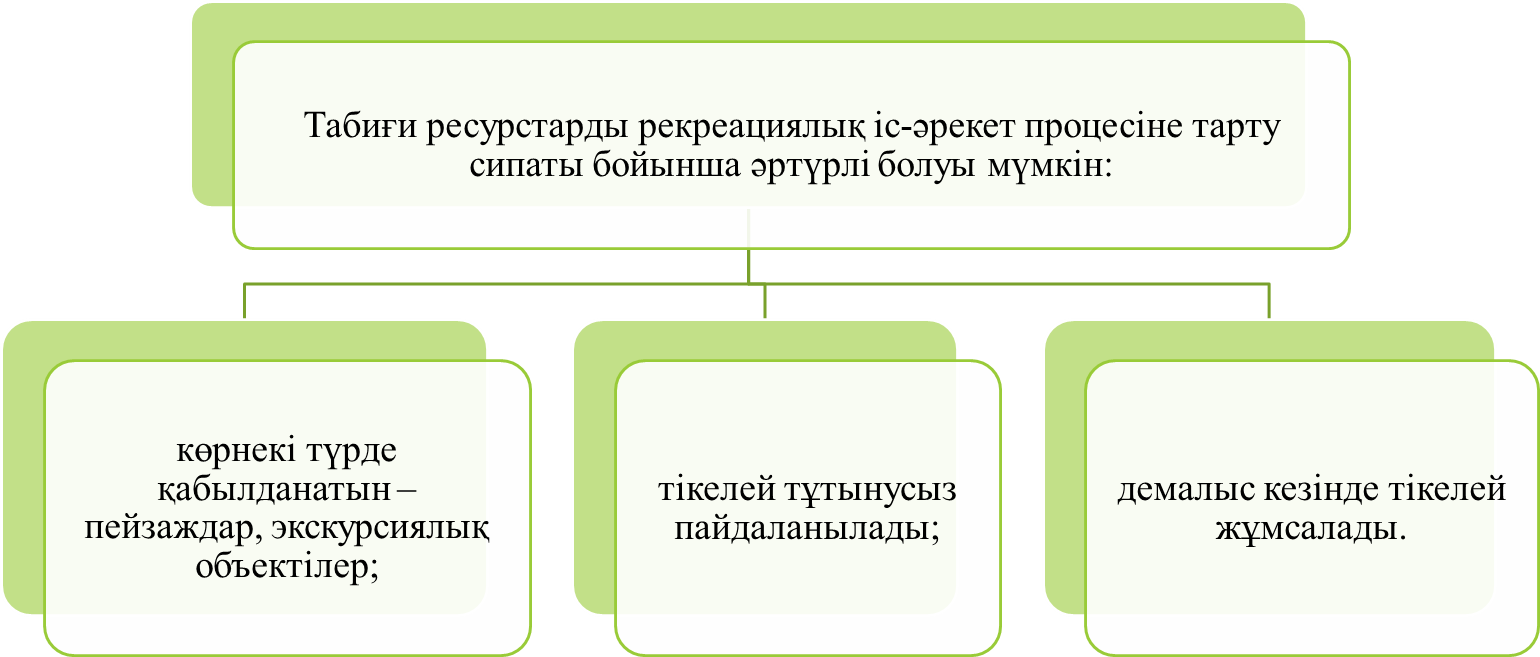
\includegraphics[width=0.8\textwidth]{assets/1111}
	\caption*{}
\end{figure}

{\bfseries Сурет 1 -- Табиғи ресурстарды рекреациялық іс-әрекеттері
{[}6{]}}

Физикалық рекреациялық ресурстар - бұл физикалық-географиялық
ресурстарға (геологиялық, геоморфологиялық, климаттық, гидрологиялық
және жылулық) жіктелген жансыз табиғаттың барлық компоненттері.

Биологиялық рекреациялық ресурстар -- тірі табиғаттың барлық құрамдас
бөліктері, соның ішінде топырақ, фаунистік және флористикалық.

Энергетикалық-ақпараттық рекреациялық ресурстар - бұл аумақты немесе
ландшафтты тарту факторлары ретінде қызмет ететін және адамның
психофизикалық жағдайына жағымды әсер ететін ноосфералық сипаттағы нақты
өрістер. Ресурстың бұл түрі мәдени, сезімтал және діни туризмді
дамытудың негізі болып табылады.

Олардың әрқайсысы табиғи (қорықтар, өзен аңғарлары және т.б.),
табиғи-антропогендік (саябақтар, скверлер, орман саябақтар, ұлттық
парктер және т.б.) және бірегей ресурстар болып бөлінеді.

Бірегей күрделі рекреациялық ресурстар табиғи және табиғи-антропогендік
ландшафттардан жасанды түрде оқшауланған. Бұл рекреациялық-бағдарланған
экономиканы дамыту үшін ең тартымды туристік орындар бола отырып,
бірегей ресурстардың (табиғат ескерткіштері) ерекше маңызы бар
екендігімен түсіндіріледі.

Осы негізде табиғи рекреациялық ресурстардың түрлері анықталады:
геологиялық, геоморфологиялық, климаттық және т.б (сурет 2).

\begin{figure}[H]
	\centering
	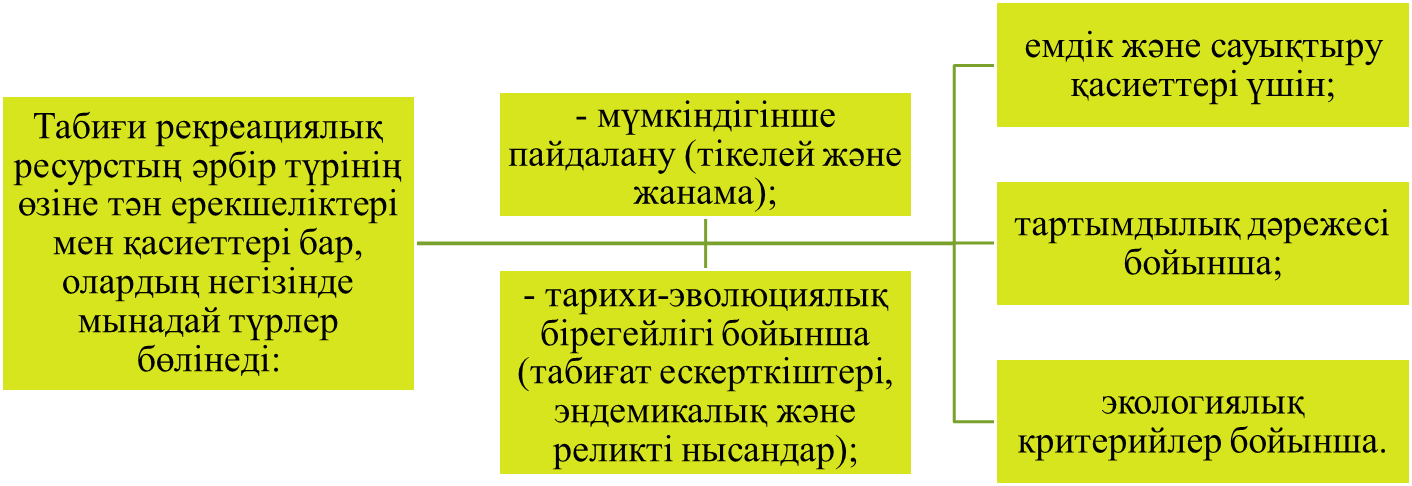
\includegraphics[width=0.8\textwidth]{assets/1112}
	\caption*{}
\end{figure}

{\bfseries Сурет 2 -- Табиғи рекреациялық ресурстарға тән ерекшіліктері
{[}7{]}}

Экономикалық бағалау үшін табиғи рекреациялық ресурстарды пайдалану
мүмкіндігін анықтау қажет. Тікелей рекреациялық ресурстар деп адамның
физикалық және рухани күшін қалпына келтіруге және дамытуға тікелей
ықпал ететін табиғат күштері түсініледі. Оларға геоморфологиялық,
климаттық, гидрологиялық және энергетикалық ақпарат, флористикалық,
фаунистік және кешендік жатады. Жанама рекреациялық ресурстар тікелей
ресурстардың қалыптасуына әсер етеді. Оларға геологиялық, топырақтық,
ішінара геоморфологиялық, энергетикалық ақпарат, флористикалық және
фауналық жатады. Кешенді табиғи рекреациялық ресурстар -- адамның рухани
және дене күшін қалпына келтіру үшін медициналық, биологиялық,
эстетикалық және ғылыми құндылығы бар, бір-бірімен зат және энергия
ағындары арқылы ажырамас байланысқан барлық табиғи рекреациялық
ресурстардың жиынтығы.

Бір аймақта немесе бір аумақта жиналған табиғи рекреациялық ресурстардың
жиынтығы болған жағдайда ғана бұл аумақты рекреациялық санатқа жатқызуға
болады немесе біртұтас кешенді табиғи рекреациялық ресурс ретінде
қарастыруға болады. Рекреациялық ресурстар неғұрлым әртүрлі болса,
аймақтың рекреациялық әлеуеті және оның экономикалық даму мүмкіндіктері
соғұрлым жоғары болады.

Экономиканың туристік-рекреациялық секторының пайда болуы мен дамуының
маңызды шарты туристік және рекреациялық ресурстар мен қызметтерге
сұраныс, сондай-ақ аймақтың қолжетімділігі мен дамуы болып табылады, ол
көбінесе географиялық орналасуы мен мемлекетімен анықталады. туризм және
рекреациялық инфрақұрылым. Табиғи рекреациялық ресурстардың әрқайсысы
басқа табиғи ресурстармен үйлескенде ғана және адамның рухани және
физикалық күшін қалпына келтіру үшін пайдаланылуы мүмкін табиғи
ресурстардың кез келгені табиғи ресурстармен үйлескенде ғана тиімді
екенін атап өткен жөн. Бұл қасиетке ие болмаса, бұл әлеуетті
рекреациялық ресурс талап етілмейтін болып қалады. Демек, рекреациялық
болмайды. Мысал ретінде Солтүстік Мұзды мұхит жағалауында орналасқан
гидроминералды бұлақтарды және т.б.

Табиғи рекреациялық ресурстар міндетті пайдалану критерийі бойынша да
жіктеледі. Технологиялық міндетті немесе қажетті және технологиялық
таңдаулы немесе ілеспе табиғи рекреациялық ресурстар ажыратылады.
Бірінші топқа рекреациялық қызметтің белгілі бір түрін жүзеге асыру
мүмкін болмайтын ресурстар жатады, мысалы, қарлы тау шыңдары шаңғы
туризмі үшін қажет.

Екінші топқа рекреациялық процеске тікелей қатыспайтын, бірақ онсыз
рекреациялық процесс мүмкін емес ресурстар жатады, мысалы, таза ауыз
судың жеткілікті мөлшері, кірме жолдарды салуға қолайлы таулы жер және
т.б.

Туристік орталықтардың тұрақты дамуы үшін біртұтас рекреациялық кешенге
кіретін барлық қолда бар рекреациялық ресурстарды есепке алу мен
бағалаудың жүйелі тәсілінің маңыздылығы жоғары. Соңғысы барлық табиғи
рекреациялық ресурстар туралы мәліметтерді жинауға, олардың экономикалық
бағасын жүргізуге және болашаққа болжам жасауға мүмкіндік беретін
ақпараттық жүйелерді дамытпай мүмкін емес.

Туристік бизнесті жүзеге асыру негізгі компоненттер: капитал, заманауи
технологиялар, адам ресурстары, туристік табиғи және мәдени-тарихи
ресурстар болған жағдайда табысты жүзеге асырылуы мүмкін. Іс жүзінде
туристік аумақтарды дамыту үшін факторлар кешені қажет. Бұл қаржылық
ресурстарды тарту және заманауи технологияларды қолдану жеткіліксіз
екенін білдіреді, ең алдымен, қажетті ресурстар бар орынды таңдау немесе
оны құру керек, бұл туристік аймақтарды маркетингтің ең маңызды міндеті.
Туристік бағыттар орналастыру мүмкіндігіне қарай екі санатқа бөлінеді.
Біріншісіне туристерді көп қабылдай алатын ірі қалалар, екіншісіне
аумағы шектеулі, туристерді қабылдау мүмкіндігі шектеулі жерлер жатады.
Екінші типтегі аумақтарға теңіз жағалаулары, тау курорттары, ұлттық
саябақтар, табиғи қорықтар жатады, оларда ауданның экологиялық
тепе-теңдігін сақтау қажеттілігіне байланысты туристерді қабылдау
мүмкіндіктері шектеулі {[}8{]}.

Сонымен қатар, барлық туристік ресурстар шексіз емес, олардың белгілі
бір көлемі (потенциалды резерві), пайдалану уақыты, пайдалану
жағдайлары, құны бар екенін атап өткен жөн. Демек, туризм және
рекреациялық ресурстық ғылым арнайы зерттеу саласы ретінде туристік және
рекреациялық ресурстарды пайдалану және қорғау шарттарын анықтауды,
бағалауды және дамытуды қамтуы керек. Дегенмен, туристік аумақтардың
имиджін қалыптастыру мәселелері зерттеудің бастапқы кезеңінде ғана,
туристік аумақтардың имиджімен кәсіби негізде айналысқан отандық
мамандар іс жүзінде жоқ. Сонымен бірге туристік аймақтың ойластырылған
бейнесін жасау оның тұтынушылар алдында құндылығын арттырады, бұл өз
кезегінде нарықтық құнын арттырады. Аумақтың құнын және оның нарықтық
құнын арттыруда аумақтардың туристік-рекреациялық ресурстары ерекше рөл
атқарады.

Туристік ресурстар да шартты түрде табиғи, яғни табиғи шығу тегі және
адам әрекетінің нәтижесінде жасалған жасанды болып бөлінеді. Туризм мен
рекреацияның серпінді дамуы екі ресурстың да дамуын талап етеді, өйткені
табиғи ресурстардың өте жоғары құндылығының өзінде заманауи
инфрақұрылымның, коммуникациялардың, спорттық және демалыс орындарының
болмауы аумақтың туристік орталық ретіндегі маңыздылығына теріс әсер
етеді. Демек, толыққанды туристік аумақты қалыптастыру барлық мүдделі
тараптардың мақсатты және жүйелі іс-әрекетін талап етеді. Өз кезегінде,
туристік аумақты (орталықты) қалыптастыру бойынша ұтымды және тиімді
қызмет аумақтың туристік-рекреациялық әлеуетін бағалау саласындағы терең
зерттеулерсіз мүмкін емес, өйткені туристік аумақтардың әлеуетін болжау
туристік аумақтарды анықтауға мүмкіндік береді. Рұқсат етілетін
жүктемелер мен осы негізде аумақтардың қоршаған ортаны қорғау және
жоғалған ресурстарды молайту мақсатында шаралар әзірлеу. Мұндай
іс-шаралар туристік бизнестің табысты дамуының негізі және аумақтық
туристік өнімді өндірудің және аймақтағы инвестициялық саясаттың басым
бағыттарын жоспарлаудың бастапқы негізі болып табылады.

Облыстың ресурстық әлеуетін сауатты және тиімді басқару үшін аумақтардың
ресурстық әлеуетін бағалаудың келесі бағыттарын әзірлеу және қолдану
қажет:

- ресурстарды сандық бағалау;

- әлеуетті құрылымды, жеке потенциалды пайдалану дәрежесін бағалау;

- ресурстарды пайдалану мүмкіндіктерін бағалау.

Туристік-рекреациялық ресурстардың жай-күйін жүйелі түрде есепке алу
және олардың облыстағы туризмді дамытудағы маңызын анықтау тек
туристік-рекреациялық кадастрлар жүйесін енгізгенде ғана мүмкін болады.

Кадастр (француз тілінен аударғанда саdastre -- регистр) -- мерзімді
түрде немесе объектіге (жер, су, орман және т.б.). Туризм терминдерінің
сөздігіне сәйкес туристік ресурстар кадастры -- бұл туристік
ресурстардың жалпылама (экономикалық немесе экологиялық) тұтынушылық
(шығын немесе нүктелік) бағасы ретінде қарастырылалы.

Кадастрды құрудың негізгі мақсаты әртүрлі аймақтарда туризмді дамытудың
барлық алғышарттары мен шарттарын барынша тиімді пайдалану жолдарын
анықтау болып табылады. Ол үшін кадастр барлық туристік ресурстардың
жан-жақты сипаттамасын, оның ішінде олардың егжей-тегжейлі есепке алуын
және жіктелуін, дамудың экономикалық тиімділігін сапалық және сандық
бағалауды, пайдалануды талдауды және оның негізгі перспективаларын,
сондай-ақ туристік ресурстарды дамытудың ең маңызды шараларын қамтуы
керек. туристік және рекреациялық ресурстарды қорғау {[}9{]}.

Бұл туристік және рекреациялық ресурстардың толық сипаттамасын, олардың
тартымдылығын, көру уақытын, аумағын (көлемін), сапасын, даму немесе
пайдалану жағдайларын, уақыт бірлігінде осы ресурсты пайдалана алатын
туристер (рекреационистер) санын сандық бағалауды қамтиды. оны
сарқылтпай және экологиялық тепе-теңдікті бұзбай пайдаланудың мәні зор.
Территориялардың экономикалық дамуындағы туризм мен рекреацияның рөлін
күшейтудің заманауи жағдайында бағалау мәселелері бірінші кезектегі
мәнге ие (сурет 3).

\begin{figure}[H]
	\centering
	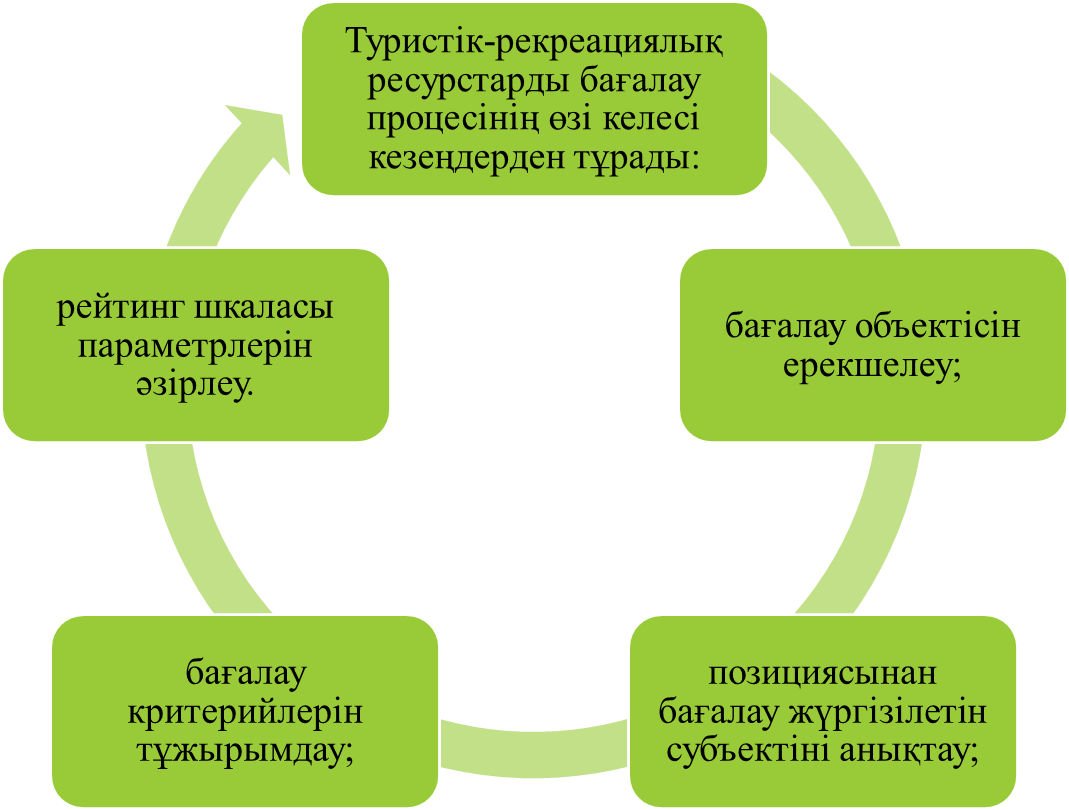
\includegraphics[width=0.8\textwidth]{assets/1113}
	\caption*{}
\end{figure}

{\bfseries Сурет 3 -- Туристік-рекреациялық ресурстарды бағалау {[}9{]}}

Шкалалар бағалау объектісі мен субъектісі арасындағы бағалау қатынасын
көрсетеді. Шкаланың 3-4 немесе 5-6 бағалау деңгейі болуы мүмкін, әрбір
деңгей берілген объектінің қасиеті мен субъектінің күйі арасындағы өзара
әрекеттесу қарқындылығының көрсеткіші болып табылады. Өзара әрекеттесу
қарқындылығы шамалыдан күштіге дейін өзгеруі мүмкін. Мәселен,
рекреацияның алғышарттарын бағалау шкаласы бес қадамнан тұрады, олардың
әрқайсысы белгілі бір градацияға сәйкес келеді:

- ең қолайлы;

- қолайлы;

- орташа қолайлы;

- аздап қолайсыз;

- қолайсыз.

Туристік және рекреациялық ресурстарды бағалаудың қолданылатын әдістері
әртүрлі, зерттеу барысында бағалаудың негізінен үш түрін қолдануға
болады: медициналық-биологиялық, психологиялық-эстетикалық және
технологиялық.

Медициналық-биологиялық бағалау табиғи факторлардың адам ағзасына әсерін
көрсетеді, мұнда климат жетекші рөл атқарады. Аумақтарды қолайлы
климаттық жағдайлар дәрежесіне қарай аудандастыруға және климаттық
терапияны кеңінен қолдануға мүмкіндік беретін, олардың адам денсаулығына
әсерін ескере отырып, климаттық факторлар кешенін бағалаудың бірқатар
әдістері әзірленді.

Психологиялық-эстетикалық бағалау табиғи ландшафт пен оның құрамдас
бөліктерінің адамға эмоционалдық әсер ету дәрежесін көрсетеді. Бұл ретте
туристік аймақта орналасқан көрікті жерлер, тарихи-мәдени және сәулет
ескерткіштері ерекше әсер етеді. Мұндай бағалау әдістері әдетте
параметрлердің әртүрлілігіне және бағалау критерийлерінің
субъективтілігіне байланысты күрделі. Дегенмен, бұл бағыттағы жұмыстар
белсенді түрде жүргізілуде, туристерді ұлттық парктердің аумақтары
бойынша бөлу зерттелуде. Бұл зерттеулердің нәтижелері шеткі аймақтардың
(екі орта арасындағы шекаралық жолақтар: су-жер (күшті әсер),
орманды-сала (орташа әсер), төбе-жазық (әлсіз әсер) ең жоғары және ең
тартымды әсер ететінін көрсетті.

{\bfseries Нәтижелер мен талқылау.} Аумақтарға географиялық-туристік талдау
жасауда рекреациялық әлеуетке жататындар:

- физикалық географиялық сипаттама бере отырып, табиғат ортасының
қолайлылығын, мүмкіндігін анықтау;

- ландшафтық жер жағдайын рекреациялық бағалай, олардың
аттрактивтілігін, экологиялық жай-күйін анықтау;

- аумақтық жергілікті тұрғыда туристік ресурстар реестрін құрастыру,
оның туристік жағдайын саралау;

- туристік-рекреациялық нысандарды пайдалану дәрежесін анықтап,
рекреациялық мүмкіндіктеріне шолу беру;

- туристік пайдалануына сай оларды аудандастыру.

Психологиялық-эстетикалық бағалаудың басқа әдістерімен қатар соңғы
уақытта экзотикалық және бірегейлік дәрежесі зерттелді. Экзотикалық
демалыс орнының тұрақты тұрғылықты жеріне қатысты қарама-қарсылық
дәрежесі ретінде, ал бірегейлік - заттардың немесе құбылыстардың
бірегейлік дәрежесі ретінде анықталады.

Технологиялық бағалау белгілі бір туризм немесе рекреация түріне
аумақтың жарамдылығын, сондай-ақ оның инженерлік және құрылыстық даму
мүмкіндігін бағалауға мүмкіндік береді.

Бағалау жұмысының қорытынды кезеңі -- интегралды бағалаудың қорытындысы
және бағалау формасын таңдау. Әдетте екі ауыспалы форма қолданылады:
сапа және нүкте. Сапалық бағалаудың күштілігі ол бағалау ерекшеліктерін
логикалық негіздеуге мүмкіндік береді. Бұл тәсіл нүктелік бағалауды
жақсырақ негіздеуге ықпал етеді, оның айрықша белгілері өрнектің
қысқалығы, анықтығы және салыстыру мүмкіндігі болып табылады.

{\bfseries Қорытынды.} Жоғарыда айтылғандарды талдай отырып, табиғи
рекреациялық ресурстар туристік өнімді қалыптастыруда орталық маңызы бар
деп айтуға болады. Алайда энергетика, көлік, байланыс, еңбек ресурстары
сияқты ресурстар көбінесе аумақ пен аймақтың рекреациялық әлеуетін
құрайды, өйткені олар мерекені жайлы, мәдениетті және қызықты өткізу.
Туристік-рекреациялық әлеуеттің негізгі қағидаттары мынадай болып
келеді. Мәселен, рекреациялық әрекеттерде оның алуан-түрлілігі туризм
жіктеліміне сәйкестігі мен оның демалу рекреациялық мүмкіндіктерін
жатқызуға болатындар:

- туристік ресурстардың өзіндік ерекшелігі, бірегейлігі;

- адамдардың қоршаған ортаға деген экологиялық көзқарасы;

- пайдаланатын ресурстардың мөлшері мен көлемі.

Рекреациялық бағалаудың жолдары әртүрлі болып келеді. Өңірдің ресурстық
әлеуетін сауатты және тиімді басқару үшін ресурстардың сандық бағасын
әзірлеу және қолдану, әлеует құрылымы мен жеке әлеуетті пайдалану
дәрежесін бағалау, пайдалану мүмкіндіктеріне нақты баға беру қажет.
Туристік ресурстардың шексіз емес екенін түсіну керек, олардың белгілі
бір потенциалдық қоры, оларды пайдалану уақыты, пайдалану шарттары мен
құны бар.

Нәтижесінде туризм және рекреациялық ресурстық ғылым туристік және
рекреациялық ресурстарды пайдалану және қорғау шарттарын анықтауды,
бағалауды және дамытуды қамтуы керек. Қазіргі уақытта туристік
аумақтардың имиджін қалыптастыруға қатысты мәселелер тек зерттеудің
бастапқы сатысында тұр және кәсіби негізде туристік аумақтардың
имиджімен айналысқан отандық мамандарды жетілдіру орынды. Сонымен бірге
туристік аймақтың ойластырылған бейнесін жасау оның тұтынушылар алдында
құндылығын арттырады, бұл өз кезегінде нарықтық құнын арттырады.
Аумақтың құнын және оның нарықтық құнын арттыруда аумақтардың
туристік-рекреациялық ресурстары ерекше рөл атқарады.

{\bfseries Әдебиеттер}

1. Ердавлетов С.Р., Искакова К.А., Артемьев А.М., Баяндинова С.М.
Рекреационный туризм: учеб. пособие. -- Алматы: Қазақ университеті,
2017. -- 214 с.

2. Зырянов А.И. Теория и методология рекреационной географии: учебное
пособие. - Пермь: Пермский государственный национальный
исследовательский университет, 2021. - 368 с.

3. Назаркина В.А., Владыкина Ю.О., Воротникова Е.Ю. Виды и тенденции
развития туризма: учебное пособие. -Новосибирск: Новосибирский
государственный технический университет, 2014. - 235 с.
ISBN978-5-7782-2437-7

4. Плохих Р.В., Исаков Е.Д., Актымбаева А.С. Туризмология негіздері: оқу
құралы. -- Алматы: Қазақ Университеті, 2021. -- 112 б.

5. Абишева З. М. Основы туристско-краеведческой работы: учебное пособие.
-- Алматы, «Қазақ университеті», 2018. -- 106 с.

6. Уварова А.К., Сабиров Д.З. Туристік-рекреациялық картографиялау курсы
бойынша лабораториялық және тәжірибелік жұмыстарды орындау нұсқаулығы.
-- Алматы: Қазақ университеті, 2016. -- 138 б.

7. Абишева З.М., Абдреева Ш.Т. Туристік өлкетану жұмыстарының негіздері:
оқу құралы. -- Өңд. толықт. 2-бас. -- Алматы: Қазақ университеті, 2019.
-- 122 б.

8. Артемьев А.М. Абдреева Ш.Т., Актымбаева А.С. Методические
рекомендации по определению норм рекреационных нагрузок на туристские
маршруты и экологические тропы особо охраняемых природных территорий
ПРООН. - Нур-Султан, 2020 г. -- 78 с

9. Шәкен А.Ш. Ердавлетов С.Р. Туризм Казахстана: учебное пособие. -
Алматы, Бастау 2015. -- 520 с

{\bfseries References}

1. Erdavletov S.R., Iskakova K.A., Artem\textquotesingle ev A.M.,
Bayandinova S.M. Rekreatsionnyi turizm: ucheb. posobie. -- Almaty: Kazak
universitetі, 2017. - 214 s {[}in Kazakh.{]}

2. Zyryanov A.I. Teoriya i metodologiya rekreatsionnoi geografii:
uchebnoe posobie. - Perm\textquotesingle: Permskii gosudarstvennyi
natsional\textquotesingle nyi issledovatel\textquotesingle skii
universitet, 2021. - 368 s. {[}in Russian{]}

3. Nazarkina V.A., Vladykina Yu.O., Vorotnikova E.Yu. Vidy i tendentsii
razvitiya turizma: uchebnoe posobie. -Novosibirsk: Novosibirskii
gosudarstvennyi tekhnicheskii universitet, 2014. - 235 s.
ISBN978-5-7782-2437-7 {[}in Russian{]}

4. Plokhikh R.V., Isakov E.D., Aktymbaeva A.S. Turizmologiya negіzderі:
oku kuraly. -- Almaty: Kazak Universitetі, 2021. -- 112 b. {[}in
Kazakh.{]}

5. Abisheva Z. M. Osnovy turistsko-kraevedcheskoi raboty: uchebnoe
posobie. -- Almaty, «Kazak universitetі», 2018. -- 106 s. {[}in
Russian{]}

6. Uvarova A.K., Sabirov D.Z. Turistіk-rekreatsiyalyk kartografiyalau
kursy boiynsha laboratoriyalyk zhane tazhіribelіk zhumystardy oryndau
nuskaulygy. -- Almaty: Kazak universitetі, 2016. -- 138 b. {[}in
Kazakh.{]}

7. Abisheva Z.M., Abdreeva Sh.T. Turistіk өlketanu zhumystarynyn
negіzderі: oku kuraly. -- Ond. tolykt. 2-bas. -- Almaty: Kazak
universitetі, 2019. -- 122 b. {[}in Kazakh{]}

8. Artem\textquotesingle ev A.M. Abdreeva Sh.T., Aktymbaeva A.S.
Metodicheskie rekomendatsii po opredeleniyu norm rekreatsionnykh
nagruzok na turistskie marshruty i ekologicheskie tropy osobo
okhranyaemykh prirodnykh territorii PROON. - Nur-Sultan, 2020 g. -78 s.
{[}in Russian{]}

9. Shәken A.Sh. Erdavletov S.R. Turizm Kazakhstana: uchebnoe posobie. -
Almaty, Bastau 2015. -- 520 s. {[}in Russian{]}

\emph{{\bfseries Авторлар туралы мәліметтер}}

Д.И. Джангельдина -- п.ғ.к., доцент, Қазақ технология және бизнес
университеті, Астана, Қазақстан, e-mail: dariga\_da@mail.ru;

С.М. Рустемова -- магистр, аға оқытушы, Қазақ технология және бизнес
университеті, Астана, Қазақстан, e-mail: sabiruwa1986@mail.ru;

Е.Б. Абеуханова -- магистр, аға оқытушы, Қазақ технология және бизнес
университеті, Астана, Қазақстан, e-mail: erkejana77@mail.ru;

К.А. Омарова -- магистр, аға оқытушы, Қазақ технология және бизнес
университеті, Астана, Қазақстан, e-mail: omarova820204@mail.ru;

Г.Б. Ахметова -- магистр, аға оқытушы, Қазақ технология және бизнес
университеті, Астана, Қазақстан, e-mail: galiya\_hanum @mail.ru.

\emph{{\bfseries Information about the authors}}

D.I. Dzhangeldina -- Ph.D., Associate Professor, Kazakh University of
Technology and Business, Astana, Kazakhstan, e-mail: dariga\_da@mail.ru;

CM. Rustemova -- Master's degree, senior lecturer, Kazakh University of
Technology and Business, Astana, Kazakhstan, e-mail:
sabiruwa1986@mail.ru;

E.B. Abeukhanova -- Master's degree, senior lecturer, Kazakh University
of Technology and Business, Astana, Kazakhstan, e-mail:
erkejana77@mail.ru;

K.A. Omarova -- Master's degree, senior lecturer, Kazakh University of
Technology and Business, Astana, Kazakhstan, e-mail:
omarova820204@mail.ru;

G.B. Akhmetova -- Master's degree, senior lecturer, Kazakh University of
Technology and Business, Astana, Kazakhstan, e-mail: galiya\_hanum
@mail.ru.

\emph{{\bfseries \hfill\break
}}\newpage
{\bfseries МРНТИ 82.33.10}

{\bfseries ЭКОНОМИКА В «ДУХОВНОМ ИЗМЕРЕНИИ» И НОВАЯ «БИЗНЕС МОДЕЛЬ»}

{\bfseries Х. Батцэнгэл}

Монгольский университет поствысшего образования, Улан-Батор, Монголия,

e-mail: esbise@yahoo.com

В современных условиях экономика как система существенно изменяется, что
обуславливает ее переход к новой экономике. Экономические исследования
нуждаются в разработке новых теоретических и методологических проблем,
приложении их к развитию бизнес модели и созданию новой, где не только
экономические выгоды, но духовное начало становятся основой деятельности
человека и организации. Духовность заложена в экономике, но более
глубокий ее анализ возможен на основе современных теорий систем и
использования методологических возможностей, представленных достижениями
естественных наук в анализе нелинейней, неустойчивой, сложной системы.
Таковой представляется современная экономика, основанная на знаниях и
духовных ценностях.

{\bfseries Ключевые слова:} знание, духовность, потециал человека, система,
прерывность, нелинейность, неустойчивость

{\bfseries «РУХАНИ ӨЛШЕМДЕГІ» ЭКОНОМИКА ЖӘНЕ ЖАҢА «БИЗНЕС-МОДЕЛЬ»}

{\bfseries Х. Батцэнгэл}

Моңғол жоғары оқу орнынан кейінгі білім беру университеті, Ұлан-Батор қ,
Моңғолия,

e-mail: esbise@yahoo.com

Қазіргі жағдайда экономика жүйе ретінде айтарлықтай өзгереді, бұл оның
жаңа экономикаға көшуіне әкеледі. Экономикалық зерттеулер жаңа теориялық
және әдіснамалық мәселелерді әзірлеуді, оларды бизнес-модельді дамытуға
және жаңасын құруға қолдануды қажет етеді, мұнда экономикалық пайда ғана
емес, рухани бастама адам мен ұйымның негізіне айналады. Руханилық
экономикада жатыр, бірақ оны тереңірек талдау жүйелердің заманауи
теориялары мен сызықтық емес, тұрақсыз, күрделі жүйені талдауда
жаратылыстану ғылымдарының жетістіктерімен ұсынылған әдістемелік
мүмкіндіктерді пайдалану негізінде мүмкін болады. Бұл білім мен рухани
құндылықтарға негізделген заманауи экономика.

{\bfseries Түйін сөздер:} білім, руханият, адамның әлеуеті, жүйе, үзіліс,
сызықтық емес, тұрақсыздық

{\bfseries THE ECONOMY IN THE "SPIRITUAL DIMENSION" AND THE NEW}

{\bfseries "BUSINESS MODEL"}

{\bfseries Kh. Battsengel}

Graduate University of Mongolia, Ulanbaatar, Mongolia,

e-mail: esbise@yahoo.com

In modern conditions, the economy as a system is changing significantly,
which causes its transition to a new economy. Economic research needs to
develop new theoretical and methodological problems, apply them to the
development of a business model and create a new one, where not only
economic benefits, but the spiritual principle become the basis of human
and organizational activity. Spirituality is embedded in economics, but
a deeper analysis of it is possible on the basis of modern theories of
systems and the use of methodological possibilities presented by the
achievements of natural sciences in the analysis of a nonlinear,
unstable, complex system. Such is the modern economy based on knowledge
and spiritual values.

{\bfseries Keywords:} knowledge, spirituality, human potential, system,
discontinuity, nonlinearity, instability

{\bfseries Введение.} Проблема духовности в основном рассматривается в
философских и других аспектах, чем в экономическом. Хотя на различных
этапах развития экономической теории вплоть до ее современных
направлений проблема эта так или иначе присутсвовала в экономических
исследованиях или по крайней мере предполагалась как общий фон,
поскольку экономику просто нельзя понять отдельно от человека, его
внутреннего мира. Последний в самом общем виде можно представить как
духовность, где потенциал человека во всем своем многообразии и развитии
получает воплощение и проявление. Если знание, даже самое глубокое,
ограничено в реализации потенциала человека, то духовность способствует
более полному его раскрытию и развитию, выражая прежде всего целостность
и взаимообогащение всех составляющих внутренного мира человека.

Знание, его воплощение в разных формах, по сути своей охватывает не весь
спектр потенциала человека к труду, созданию и накоплению богатства, в
том числе духовного. Что касается духовности, то она пронизывая все
заложенные в человеке способности, обеспечивает их духовную целостность,
тем самым позволяет более полной их реализации в экономике. Духовность в
этом контексте можно определить как качество человека, позволяющее
обеспечить как бы ``синергию'' различных способностей и энергии человека
как целостной личности. В этой связи экономику нужно рассматривать не
только с точки зрения затрат и результатов деятельности, но и
потребления энергий, заложенных в человеке. Потенциал человека в таком
понимании можно представить как ``сгусток'' энергии самого различного
типа, начиная с энергии, создающие экономику как самоорганизующуюся и
саморазвивающуюся систему.

{\bfseries Материалы и методы.} В приложении к экономике идеи ее
энергетической природы выдвигали исследователи и раньше. Один из первых,
кто последовательно разработал данную проблему был экономист, философ
С.А. Подолинский(1850-1891), рассматривающий труд как особенный процесс,
который ``улавливает'' тот или иной поток энергии, превращает энергии
природы и человека в экономическое и духовное богатство. Тем самым
становится усилителем потенциала человека, основой раскрытия и развития
его способностей, что позволяет рассмотреть экономику, ее трудовую
природу и как духовно-нравственную категорию. По определению С.А.
Подолинского, ``Труд есть такое потребление механической и психической
работы, накопленной в организме, которое имеет результатом увеличение
количества превратимой энергии на земной поверхности'' {[}1{]}. В его
понимании ``увеличение количества превратимой энергии'' происходит через
увеличение и духовной энергии человека, без которой не могут быть
раскрыты и развиты его самые разносторонние способности к труду,
созданию капитала, других благ.

Не даваяся в суть его концепции экономики и ее энергетической природы
отметим, что он представлял труд как всякая полезная деятельность,
особенный процесс превращения энергии в конкретные блага, материальные,
духовные и т.д. Это уже возвышает понимание экономики, ее духовности на
новый уровень в отличии от классической экономической теории, где труд
рассматривается прежде всего как промышленный, полезность его в создании
благ, приносящих прибыль. Однако классическое понимание труда до сих пор
остается методологической основой и многих современных направлений
экономической теории без существенных изменений и дополнений, разве что
отмечается влияние технологической структуры современной экономики на
содержание труда, динамику и структуру занятости, более того и на всю
институциональную систему.

Осмысление труда и экономики в контексте их энергетической природы
позволяет представить, что полезность не ограничивается лишь чисто
экономической выгодой. Поскольку она есть результат потребления энергии,
заложенных не только в человеке, но и в природе, по определению
С.А.Подолинского, и космической энергии. Поэтому бизнес модель в силу
своих духовных составляющих, вполне может быть ориентирована на духовные
ценности помимо экономической выгоды. Возможность переориентации бизнес
модели или создания новой обусловлена тем, что духовность изначально
присуща экономике как системе. Другой вопрос -- почему на ней не
ставится акцент в целеполагании бизнес модели, каков механизм ее
функционирования и раскрытия в экономике, как задействовать данный
механизм в полную ``мощность''.

{\bfseries Результаты и обсуждение.} В современной бизнес модели все
отчетливо просматривается тенденция сочетать экономические выгоды с
другими ориентирами, в часности, решеиием социальных вопросов,
повышением социальной ответственности и т.д. Это очень важные изменения,
происходящие в бизнес модели самых различных типов. Но ``сидит'' на двух
стульях одновременно просто невозможно. Акцент должен ставиться на
одном, а другие должны из него исходить или ему подчиняться. Такова
логика ``функционирования'' духовности в экономике. До сих пор в рамках
существующей системы экономических координат мы старались сочетать
разные векторы развития, что давало лишь краткосрочные результаты.

В целополагании бизнес модели, где и как ставить акцент -- важный
вопрос, от решения которого во многом зависит переориентация бизнес
модели в нужном нам направлении. Неслучайно, что все значительные идеи
бизнеса, инновационные начинания, создание новых продуктов и производств
возникают как будто спонтанно, лишь от тех идей и мыслей, что постоянно
хотелось делать и воплотить в жизнь, создать и произвести, от
создаваемого внутри самого себя, в своей ``душе'' ``интелектуального
образа''. Таким образом, вначале создается образное представление, как
их реализовать и осуществить на деле, т.е. ``технологию'' их создания и
производства внутри себя. Такая внутренняя духовная, интелектуальная
работа во многом предшествует возникновению и формированию новых идей,
новой бизнес модели. Не экономическая необходимость, выгода, а именно
такое духовное начало определяет основную линию поведения многих
успешных, тем более инновационных компаний.

Экономика как общая система в каждой отдельно взятой своей единице по
особому превращает космическую энергию, по Подолинскому, посредством
человеческого труда в те или иные виды богатства, самые разнообразные
духовные ценности, в различные сочетания бизнес моделей и даже методов
управления, типов менежмента. Понятие ``различные сочетания'' в данном
случае не означает, что в какой то бизнес модели или системе управления
можно одновременно задействовать все силы и факторы без выделения
исходной точки, откуда начинается их действие и расходятся все
координаты. Такой точкой является духовное начало в экономической
системе, которое представляется как мысль, возникшая, образно говоря, от
``сердца'', в душе человека.

Мысль эта начинается с восприятия, которое не является просто актом
собирания информации, восприятия разнообразных сигналов извне, а прежде
всего результатом активного контакта с внутренним миром человека,
трансформации составляющих его мыслей и их взаимодействия. Одним словом
``хаос'' мыслей, если применить идеи И.Пригожина относительно механизма
``хаоса'' в системе, переходит к выделению основной линии, координата
динамики системы, т.е. возникновению и оформлению главной мысли, от
которой сталкиваются или расходятся другие{[}2{]}. Отсюда вывод, что для
новой бизнес модели важен способ улучшения возможностей восприятия
экономических агентов, которые должны развивать необходимую
чувствительность, находить способы развития своей духовной,
интелектуальной памяти о прошлом, настоящем и будущем. На этой основе
экономические агенты претерпевают внутренние структурные изменения
убеждений, идей и духовных установок, решат, что в каком бизнесе будут
участвовать или свой бизнес начинут своим умом и сердцем, а не только в
силу экономической необходимости, лишь опираясь на ``разум'', знание и
опыт. Такое взаимодействие с окружающей средой и своим внутренним миром
возможно на духовной основе, что заставляет их раскрыть полнее свои
способности и таланты, бизнес организациям выживать в конкурентной среде
и развивать свой потенциал, приспосабливаться к меняющему миру.

Поэтому от того, какая мысль стала началом построения той или иной
бизнес модели зависит, каким будет ее содержание и цель, направленность
деятельности. Если из всего многообразия и ``хаоса'' возникших во
внутреннем мире человека мыслей, их взаимодействия вы будуте следовать
мысли о своей выгоде, то у вас строится бизнес модель, где не человек, а
потребители становятся главным объектом приложения энергии, в том числе,
духовной. Когда мысль о том, чтобы работать не просто на обеспечение
потребностей человека, прежде всего на самого человека становится
основной, то строится другая бизнес модель, которую можно называть как
``новую''. Здесь духовность определяет основные координаты в развитии
экономики, что не противоречит экономическому развитию как таковому.
Просто последнее подчиняется первому, что делает саму экономическую
систему действительно динамичной, самоорганизующейся.

В современных условиях экономика как система существенно изменяется, что
довольно интенсивно и с разных теоретико-методологических позиций
анализируется учеными-экономистами. Во многих исследованиях изменение
системы рассматривается как переход к новой экономике, где основным
фактором развития становится знание. Знание более других факторов
связано с духовным началом экономики, что делает влияние духовности на
экономику значимым и важным. Это проявляется прежде всего в
переориентации экономического развития на всех уровнях, что отражается
на целевых установках экономических агентов. Однако проблема духовности
в такой постановке не всегда последовательно проработывается
исследователями в теоретическом анализе происходящих изменений в самой
экономической системе, так и в осмыслении глубиннных причин эволюции
экономической теории, которая при всем своем развитии и изменении, все
еще остается продолжением теории ``материальной цивилизации'', суть
которой, определенная французским историком Фернан Броделью до сих пор
остается основной парадигмой развития общества{[}3{]}. Даже во многом
теоретические разработки так называемой ``новой'' экономики, основанной
на знании, идут в русле той же парадигмы экономического развития,
возникшей в эпоху индустриальную. И сегодня мы живем при всех
кардинальных изменениях в той же ``материальной цивилизации'', в
обществе индустриальном, за их рамки по существу не входят все эволюция
и развитие экономики, даже переход к экономике, основанной на знаниях.

Теоретическое осмысление духовности в экономике дает возможность
взглянуть за рамки экономики, созданной ``материальной цивилизацией'',
индустриальным обществом и по новому представить переход к экономике,
основанной на знаниях. В данной постановке, переход этот означает
глубинные изменения, происходящие в самой основе экономики, где духовное
начало становится все более значимым. Это трансформируется и в
постепенную переориентацию существующей бизнес модели и создание новой.
В этой связи проблему измерения следует разработать с учетом такой
переориентации бизнес модели. Для этого важно исходит из положения, что
духовность в самом первом приближении измеряется тем, насколько полнее
раскрыт и реализован человеческий потенциал, потенциал бизнес
организации, какое количество энергий, заложенных в человеке и природе
превращено человеческим трудом в конкретные блага, какова полезность
труда и деятельности организации не только для потребителей, а именно в
том, насколько и в какой мере она направлена на человека.

Постановка проблемы в такой плоскости требует других методологических
подходов к ее разработке, поскольку теоретическое объяснение которой
возможно с точки зрения рассмотрения экономики как ``живой'' системы.
Хотя традиционное трехмерное представление экономики как взаимодействие
таких факторов как земля, труд и капитал, последовательно сменяется
теоретическим обоснованием экономики знаний. Однако даже это не может в
полной мере объяснено лишь происходящим переходом к экономике знаний и
тем, что знание становится основным фактором экономического развития. В
основе происходящего перехода лежат более глубинные причины и системные
преобразования общества, которые правомерно анализировать в контексте
современных теорий систем, используя новые возможности, представленные
развитием методологии системных исследований прежде всего в естественных
науках {[}4{]}. Эти методологические возможности следует последовательно
приложить к анализу проблемы экономики в ``духовном измерении'' и
``новой'' бизнес модели.

Забегая впредь отметим, что в экономической теории до сих пор
сохраняется традиционный подход к пониманию непрерывности движения как
основной характеристики развития. Однако надо признать, что в
современных исследованиях делаются попытки переосмысления данной
проблемы в контексте экономики как динамической системы, более того
признания прерывности и перехода к другой системе. Непрерывность
движения в экономике есть частность в линейнем развитии, что
противоречит динамической характеристике системы. Неслучайно, на
практике и в обосновании экономической политики такое понимание
экономики всегда допускает неизбежность волнообразного поведения
экономики, кризисных явлений и цикличного развития, соответственно и
строятся различные бизнес модели. Что касается прерывность развития как
состояние нелинейнной модели экономического развития, то такой подход к
анализу экономики как системы позволяет выяснить внутренний механизм
экономического развития, где духовное начало становится точкой раскрытия
заложенных в экономике энергий, если использовать определение А.С.
Подолинского.

Такое положение вещей объясняется в современной теории систем как
``хаос'' переходит к порядку и наоборот. Тот же механизм действует
внутри экономической системы, их различных моделей в разных странах и
регионах. Различие в духовных ценностях, системах мышления и
мировозрения, культурах и нравственных принципах народов как ``хаос'' в
миросистеме определяет все богатство и разнообразие духовности в мировой
экономике, что в каждой отдельно взятой единице экономики, то конкретный
человек или организация выдвигает на первый план те или иные координаты
и направления действий. Не случайно, одна и та же бизнес модель, один и
тот же тип менеждмента, одни и те же методы управления в разных странах
и регионах, на различных предприятиях и организациях имеют свои
особенности, что чрезвычайно важно учесть при всей их общности. Отсюда
вывод -- достичь каких то видимых, долгосрочных результатов не возможно
на основе механического использования даже самых лучших бизнес моделей,
методов и форм управления, более того моделей экономичекого равития без
тщательной предварительной духовной, интелектуальной работы у себя, их
приспособления соотвественно своей духовной, интелектуальной структуре
мышления.

Проникновение в экономику новых идей и методов из областей системных
исследований и развития методологии, более развитых в естественных
науках, в частности, физической и биологической науки позволяет
определить нелинейнность, прерывность, неустойчивость как основные
характеристики ``живой'' экономической системы. Такое понимание
экономической динамики существенно расширает горизонты экономического
анализа за рамки традиционных подходов и позиций, где свое ``законное
место'' может занять и духовность в экономике.

При этом нужно отметить, что динамика системы делает любой переход от
одного состояния в другое чрезвычайно противоречивым и сложным. Это
следует учесть в анализе проблем преобразования современной экономики и
перехода к новой бизнес модели в частности. На такое противоречие,
присущее нелинейной, сложной системе указывал один из основателей
нелинейной науки В.И. Арнольд. Как писал В.И.Арнольд, в нелинейной
системе при переходе из одного устойчивого состояния в другое, более
предпочтительное: 1) постепенное движение к лучшему состоянию сразу
приводит к ухудшению и его скорость при равномерном движении
увеличивается, при этом сопротивление изменению растет; 2) сопротивление
достигает максимального значения раньше перехода через наихудшее
состояние; 3) величина ухудшения, необходимая для перехода в лучшее
состояние, сравнима с финальным улучшением {[}5{]}.

В этой связи и духовность следует рассматривать как свойство экономики,
понимаемой как нелинейной, сложной системы. Поэтому в духовности
присутствует не только ``хаос'' самых различных мыслей и идей, исходящих
из внутренного мира человека, а также их превращение в реальные
действия, те или иные материальные, духовные и другие блага представляет
на деле такой же противоречивый переход от одного устойчивого состояния
в другое. Духовность не только опирается на разум, но прежде всего на
гармонию всех составляющих потенциала и способностей человека, что
обуславливает внутренний мир, внутреннюю культуру. Соответственно бизнес
модель получает другое содержание, где упор ставится не просто на
потребностей как таковых, а именно на развитии человека и т.д. Вместо
прибыльности, доходов, бизнесменов интересует не просто экономические
параметры, но и духовные {[}6{]}.

Экономические целеуказания дополняются духовными ориентирами,
направленностью, которые в свою очередь постепенно делают одухотворенной
саму экономическую деятельность, начиная с индивидуального труда, бизнес
организаций и т.д. Здесь духовным началом такой переориентации
становится свободный выбор деятельности по ``зову сердца'', от души, от
понимания того, что человеку или бизнес организации хочется делать,
какая деятельность позволит им саморазвиваться и совершить то, что
хочется, а не в зависимости от чисто экономической выгоды. Такие
возможности в условиях перехода к экономике, основанной на знаниях
существенно увеличиваются и данная тенденция в дальнейшем усилится еще
больше, хотя бы в силу развития новых технологий, дающих все более
широкие поля для самостоятельного, свободного от навязанных традиционным
разделением труда выбора деятельности и создания собственных,
неповторимых, инновационных форм бизнес творчества.

{\bfseries Выводы.} В этой связи изменяется и бизнес модель, где упор будет
сделан на ориентации бизнес деятельности сначало на оптимальное
сочетание экономических и социальных составляющих в цели,
направленности, что в традиционной бизнес модели не всегда
обеспечивается. На следующем этапе происходит подчинение экономических
целей, задач или ориентации социальным. Это затронет само содержание
деятельности экономических агентов и делает их ответственныи за духовное
развитие.

В современной экономической науке недостаточно обращает внимание на то,
что исследование проблемы духовности в экономике открывает новые
концептуальные, теоретические возможности глубже понимать экономику как
``живую'' систему. В этой связи, вместо линейной модели экономического
развития, детально разработанной, удобной и понятной, с определенностью
и предсказуемостью поведения, приходит другая с неопределенностью и
ограниченной предсказуемостью. Это требует создания новой бизнес модели,
приспособленной и устойчивой к неопределенности и постоянным изменениям
экономики, где духовность как синергия всех составляющих потенциала
человека и организации становится основой такой модели.

{\bfseries Литература}

1. Подолинский С.А. Труд человека и его отношение к распределению
энергии:учебник. - М. Амрита, 2019. -132 с.

2. Пригожин И., Стенгерс И. Порядок из хаоса: Новый диалог человека с
природой / Пер. с англ. Общ. ред. В. И. Аршинова, Ю. Л. Климонтовича и
Ю. В. Сачкова. - М.: Прогресс, 1986. - 432 с.

3. Бродель Фернан. Материальная цивилизация, экономика и капитализм.
XV-XVIII вв. Учебник. -М.Альма-Матер, 2023. -- 2258 с.

4. Сорокин П.А. Социальная и культурная динамика / Пер. с англ.,
ввступ.ст. и коммент. В.В. Сапова. - М.: Академический проект, 2017. -
964 с.

5. Арнольд В.И. Математическое понимание природы: Очерки удивительных
физических явлений и их понимания математиками. - 3-е изд., стереотип. -
М.: МЦНМО, 2011. -- 144 с.

6. Морозов, В. А. Духовная экономика общества: учебное пособие. -
Москва: Дашков и К, 2023. - 2-е изд. - 458 с. - ISBN 978-5-394-05244-6.
- URL: https://znanium.com/catalog/product/1923198 (дата обращения
05.03.2024)

{\bfseries References}

1. Podolinskii S.A. Trud cheloveka i ego otnoshenie k raspredeleniyu
energii: uchebnik. - M. Amrita, 2019. -132 s. {[}in Russian{]}

2. Prigozhin I., Stengers I. Poryadok iz khaosa: Novyi dialog cheloveka
s prirodoi / Per. s angl. Obshch. red. V. I. Arshinova, Yu. L.
Klimontovicha i Yu. V. Sachkova. - M.: Progress, 1986. - 432 s. {[}in
Russian{]}

3. Brodel\textquotesingle{} Fernan. Material\textquotesingle naya
tsivilizatsiya, ekonomika i kapitalizm. XV-XVIII vv. Uchebnik.
-M.Al\textquotesingle ma-Mater, 2023. -- 2258 s. {[}in Russian{]}

4. Sorokin P.A. Sotsial\textquotesingle naya i
kul\textquotesingle turnaya dinamika / Per. s angl., vvstup.st. i
komment. V.V. Sapova. - M.: Akademicheskii proekt, 2017. - 964 s. {[}in
Russian{]}

5. Arnol\textquotesingle d V.I. Matematicheskoe ponimanie prirody:
Ocherki udivitel\textquotesingle nykh fizicheskikh yavlenii i ikh
ponimaniya matematikami. - 3-e izd., stereotip. - M.: MTsNMO, 2011. --
144 s. {[}in Russian{]}

6. Morozov, V. A. Dukhovnaya ekonomika obshchestva: uchebnoe posobie. -
Moskva: Dashkov i K, 2023. - 2-e izd. - 458 s. - ISBN 978-5-394-05244-6.
- URL: https://znanium.com/catalog/product/1923198 (data obrashcheniya
05.03.2024) {[}in Russian{]}

\emph{{\bfseries Сведения об авторах}}

Батцэнгэл Хуухээ -- доктор экономических наук, профессор, директор
Института современных исследований, Монгольский университет поствысшего
образования, e-mail: esbise@yahoo.com

\emph{{\bfseries Information about the author}}

Khukhe Battsengel -- Doctor of Economics, Professor, Director of the
Institute of Modern Studies, Graduate University of Mongolia, e-mail:
esbise@yahoo.com

\emph{{\bfseries \hfill\break
}}\newpage
{\bfseries МРНТИ 71.37.01}

{\bfseries КҮРДЕЛІ БИЗНЕС ПРОЦЕСТІ БАСҚАРУДЫҢ АҚПАРАТТЫҚ ЖҮЙЕСІ МЕН
АЙМАҚТЫҚ ДАМУДЫҢ КӨП НҰСҚАЛЫ РЕГРЕССИЯЛЫҚ ТАЛДАУЫ}

{\bfseries Ж. Бидахмет, А.Р. Исаев,}

\textsuperscript{1}әл-Фараби атындағы Қазақ ұлттық университеті, Алматы,
Қазақстан

Корреспондент-автор: aydarisaev@mail.ru

Қазіргі таңда, әлемде бізді тұтас компьютерлік инновациялар, түрлі
бағдарламалық құралдар қоршап тұр. Қызметтің барлық салаларында
ақпараттық технологиялар қолданылады. Сол сияқты,күнделікті өмірімізде
әртүрлі курорттар, демалыс және ойын-сауық орындары көбейіп келеді. Әр
жолы туристерді таң қалдыру қиынырақ, керісінше, көптеген адамдар,
сауалнамалар мен зерттеулер көрсеткендей, адамның "өркениетті аяғы"
жетпеген жердің бұрыштарына, қалалардан алыс, табиғатқа, шулы көліктер
жоқ жерде, адамдар көп емес жерде тіпті, табиғат-ананың сұлулығынан
ләззат алып саяхаттауды жөн көреді. Ал, дәл осындай жерлер кең байтақ
Қазақстанда өте көп десе де болады.

Қазақстанда туризмді дамыту үшін бірінші кезекте \emph{Ақпараттық
өрісті} дамыту қажет. Қазақстандағы туристік ақпараттық жүйелер (АЖ)
бірқатар проблемаларды бастан кешіруде, мысалы: бір типтілік,
консервативтілік және т. б.

Бұл жұмыста ақпараттық туризммен байланысты бірқатар мәселелердің
сипаттамасы, сондай-ақ шешімнің бір моделі ұсынылады. Негізгі мақсат --
көп нұсқалы регрессия әдістерін қолдана отырып, туризмнің экономикалық
өсуге, жұмыспен қамтуға және әлеуметтік инфрақұрылымның дамуына қалай
әсер ететінін сандық талдау. Деректер әртүрлі аймақтық көздерден, соның
ішінде Қазақстан Статистика агенттігінен, туризм департаментінің
жазбаларынан және 2019 және 2022 жылдар аралығында жергілікті бизнес пен
туристермен жүргізілген сауалнамалардан жиналды. Талдау туризммен
байланысты қызмет пен әлеуметтік-экономикалық нәтижелер арасындағы
қарым-қатынасты анықтау үшін көптеген регрессиялық модельдерді
пайдаланды. Зерттеу туризмнің әсерін күшейтетін негізгі факторларды,
соның ішінде инфрақұрылымды жақсартуды, қызмет көрсету сапасына
инвестицияны және тұрақты тәжірибеге бағытталған стратегиялық
маркетингті анықтайды. Бұл зерттеу басқа контекстердегі ұқсас
зерттеулердің үлгісін ұсына отырып, аз танымал аймақтардағы туризмнің
трансформациялық күшін тереңірек түсінуге ықпал етеді.

{\bfseries Түйін сөздер:} ақпараттық жүйелер, сандық талдау, сыртқы
факторлар, регрессиялық талдау, инфрақұрылымдық инвестиция,
технологиялық инновациялар, аймақтық даму.

{\bfseries МНОГОФАКТОРНЫЙ РЕГРЕССИОННЫЙ АНАЛИЗ СЛОЖНОЙ ИНФОРМАЦИОННОЙ
СИСТЕМЫ УПРАВЛЕНИЯ БИЗНЕС-ПРОЦЕССАМИ И РЕГИОНАЛЬНОГО РАЗВИТИЯ}

{\bfseries Ж. Бидахмет, А.Р. Исаев}

\textsuperscript{1}Казахский национальный университет имени аль-Фараби,
Алматы, Казахстан,

е-mail: aydarisaev@mail.ru

Сегодня, в мире, нас окружают целые компьютерные инновации, различные
программные средства. Во всех сферах деятельности используются
информационные технологии. Точно так же в нашей повседневной жизни
появляется все больше различных курортов, курортов и развлекательных
заведений. С каждым разом туристов удивлять сложнее, наоборот, многие,
как показывают опросы и исследования, предпочитают путешествовать,
наслаждаясь красотой матери-природы, в уголки Земли, куда не доходят
"цивилизованные ноги" человека, вдали от городов, на природу, там, где
нет шумных машин, там, где не так много людей. А таких мест в огромном
Казахстане очень много.

Для развития туризма в Казахстане необходимо в первую очередь развивать
информационное поле. Туристические информационные системы (ИС) в
Казахстане испытывают ряд проблем, таких как: однотипность,
консервативность и др.

В данной работе предлагается описание ряда проблем, связанных с
информационным туризмом, а также одна модель решения. Основная цель
состоит в количественном анализе того, как туризм влияет на
экономический рост, занятость и развитие социальной инфраструктуры с
использованием методов многомерной регрессии. Данные были собраны из
различных региональных источников, включая статистическое агентство
Казахстана, отчеты департамента туризма и опросы местных предприятий и
туристов в период с 2019 по 2022 год. В анализе использовалось множество
регрессионных моделей для определения взаимосвязи между деятельностью,
связанной с туризмом, и социально-экономическими результатами.
Исследование определяет ключевые факторы, которые усиливают влияние
туризма, включая улучшение инфраструктуры, инвестиции в качество услуг и
стратегический маркетинг, ориентированный на устойчивые методы. Это
исследование способствует более глубокому пониманию преобразующей силы
туризма в менее известных регионах, предлагая модель аналогичных
исследований в других контекстах.

{\bfseries Ключевые слова:} информационные системы, количественный анализ,
внешние факторы, регрессионный анализ, инвестиции в инфраструктуру,
технологические инновации, региональное развитие.

{\bfseries MULTIFACTORIAL REGRESSION ANALYSIS OF A COMPLEX INFORMATION
SYSTEM FOR BUSINESS PROCESS MANAGEMENT AND REGIONAL DEVELOPMENTRESSION
ANALYSIS OF REGIONAL DEVELOPMENT}

{\bfseries Zh. Bidakhmet, А.R. Isaev}

\textsuperscript{1}Al-Farabi Kazakh National University, Almaty,
Kazakhstan,

е-mail: aydarisaev@mail.ru

Today, in the world, we are surrounded by whole computer innovations,
various software tools. Information technologies are used in all fields
of activity. Similarly, there are more and more different resorts,
resorts and entertainment venues in our daily lives. It is more
difficult to surprise tourists every time, on the contrary, many, as
surveys and studies show, prefer to travel, enjoying the beauty of
mother nature, to corners of the Earth where "civilized feet" of man do
not reach, away from cities, to nature, where there are no noisy cars,
where there are not so many people. And there are a lot of such places
in the vast Kazakhstan.

For the development of tourism in Kazakhstan, it is necessary first of
all to develop the information field. Tourism information systems (IS)
in Kazakhstan are experiencing a number of problems, such as:
uniformity, conservatism, etc.

This paper offers a description of a number of problems related to
information tourism, as well as one solution model. The main objective
is to quantify how tourism affects economic growth, employment and
social infrastructure development using multidimensional regression
methods. The data was collected from various regional sources, including
the Statistical Agency of Kazakhstan, reports from the Department of
Tourism and surveys of local businesses and tourists between 2019 and
2022. The analysis used a variety of regression models to determine the
relationship between tourism-related activities and socio-economic
outcomes. The study identifies key factors that enhance the impact of
tourism, including infrastructure improvements, investments in quality
services, and strategic marketing focused on sustainable practices. This
study contributes to a deeper understanding of the transformative power
of tourism in lesser-known regions by offering a model of similar
research in other contexts.

{\bfseries Keywords:} information systems, quantitative analysis, external
factors, regression analysis, infrastructure investments, technological
innovations, regional development.

{\bfseries Кіріспе.} Қазіргі таңда ақпараттық технология күннен күнге
қарқынды даму үстінде. Біздің технологиялар қарқынды дамып жатқан
әлемде, компаниялардың бәсекелестік нарықта өз орнын ойып алудың басты
құралы -- ақпарат болып саналады. Ақпарат қазіргі экономикалық қызметте
есептеме басы болып табылады және де бұл кездейсоқтық емес. Ақпараттық
технологиялар заманауи өркенниеттің инфроқұрылымының барлық сыни
элементтерін басқарудың мәнін құрайды. Жаһандық экономиканың негізгі
саласы болып табылатын туризм индустриясы әлеуметтік-экономикалық
факторлардың, технологиялық жетістіктердің және жаһандық дағдарыстардың
әсерінен қалыптасатын күрделі қиындықтар мен мүмкіндіктерге тап болып
отыр. Пандемияның жаһандық туризмге трансформациялық әсерін бағалайтын
Госслинг, Скотт және Холл (2020) талдаған COVID-19 пандемиясы саланың
осалдығын және стратегиялық тұрақтылық қажеттілігін атап өтті {[}1{]}.
Бұл іргелі өзгеріс тұрақтылық пен бейімделгіштікке баса назар аудара
отырып, туристік тәжірибелерді қайта бағалауды қажет етеді. Әлемдегi
тенденцияларды ескере отырып, Қазақстанда да бұл мәселелер өзектi
проблемалардың бiреуi болып тұр деп айтуға болады.

Технологиялық инновациялар туризм индустриясында төңкеріс жасауды
жалғастыруда. Ли және т.б. (2019) туристерге нақты уақытта, теңшелген
қызметтерді ұсына отырып, туризмді басқаруды айтарлықтай жақсартатын
смарт технологиялардың интеграциясын талқылайды {[}2{]}. Сонымен қатар,
Сигала (2018) пәнаралық тәсілдер арқылы туризмді қайта құрудағы рөлін
атап көрсете отырып, жаңа технологиялардың бұзушы әлеуетін қарастырады
{[}3{]}.

Тұрақтылық туризмді дамытудың негізі болып қала береді. Budeanu және
т.б. (2016) экологиялық, экономикалық және әлеуметтік факторлар
арасындағы тепе-теңдікті жақтап, туризмдегі тұрақты тәжірибені енгізудің
қос қиындықтары мен мүмкіндіктерін зерттейді {[}4{]}. Сол сияқты,
Хиггинс-Десбиоллес (2018) әсіресе пандемия сияқты жаһандық
сын-қатерлерге жауап ретінде әлеуметтік және экологиялық әділеттілікті
насихаттайтын туристік модельді талап етеді {[}5{]}.

Экономикалық ойлар да бірдей маңызды. Брида, Кортес-Джименез, және
Пулина (2016) туризмнің әртүрлі аймақтардағы экономикалық әсері туралы
түсініктерді ұсына отырып, туризмге негізделген өсу гипотезасының
дұрыстығын қарастырады {[}6{]}.

Туризм динамикасын түсінуде теориялық негіздер де маңызды рөл атқарады.
Батлердің (1980) туристік аймақтың өмірлік циклі концепциясы туристік
бағыттардың эволюциялық кезеңдерін және олардың ресурстарды басқарудағы
салдарын зерттеуге теориялық объективті ұсынады {[}7{]}. Бұл модель осы
саладағы практикалық және эмпирикалық зерттеулерді толықтыратын іргелі
теорияны ұсынады.

{\bfseries Материалдар мен әдістер.} Күрделі жүйелер математикалық
модельдер қойылу әдістерін және оларды зерттеу тәсілдері --жаңа ғылыми
60 жылдары пайда болған. 21 --шы ғасыр заманы -- күрделі жүйелер
теориясы. Күрделі жүйелер элементтерін математикалық сипаттау үшін
функциялар теориясын, заманауи алгебраны және функционалдық анализді
пайдаланады. Күрделі зерттеуді әдетте тиімділік, сенімділік,
қауіпсіздік, басқару сапасы және басқа да күрделі жүйелердің маңызды
қасиеттері көрсеткіштері болып табылатын функционалдық сипаттамаларын
бағалаудан бастайды.Кез --келген күрделі жүйенің түйістіру сұлбасы бұл
предикаттар жиынтығы ретінде анықталады, оның элементтерінің көптеген
кірістер мен шығыстарға бөлінген, алайда күрделі жүйе құрылымын зерттеу
үшін математикалық логика және графтар теориясы аппаратын пайдаланады.
Құрылымдық анализ тәсілі күрделі жүйеден белгілі бір байланыста болған
жүйе ішіндегі жүйе тізбектерін бөліп алуға мүмкіндік береді, және
күрделі жүйені жақсы зерттелген типтік құрылымы бар объектілер жиынтығы
ретінде біле аламыз.

Жалпы бизнес процесті жобалау барысында да қолданатын жүйе күрделі жүйе
болып табылады. Бұл зерттеуге арналған деректер туризмнің әсерін
жан-жақты көрсету үшін бірнеше билік органдарынан алынды. 2010-2020
жылдар аралығында келушілер статистикасы, кіріс және маусымдық туризм
үлгілері Солтүстік Қазақстан облыстық туризм басқармасымен ұсынылды.
ЖІӨ~(жалпы ішкі өнім), жұмыспен қамту деңгейі және табыс деңгейі сияқты
экономикалық көрсеткіштер Қазақстанның Ұлттық статистика басқармасынан
алынды {[}8{]}. Жергілікті үкімет көздерінен алынған есептер көлік,
қонақжайлылық және коммуналдық инфрақұрылымдағы өзгерістер туралы
мәліметтерді қамтамасыз етті {[}9{]}. Сонымен қатар, білім беру,
денсаулық сақтаудың қолжетімділігі және өмір сапасы көрсеткіштеріне
қатысты көрсеткіштер Қазақстанның денсаулық сақтау және білім
министрлігінен алынды {[}10{]}.

Аймақтағы бірнеше әлеуметтік-экономикалық көрсеткіштерге туризмнің
әсерін зерттеу үшін көп нұсқалы регрессиялық модель қолданылды. Біздің
талдауымыздағы тәуелді айнымалыларға жан басына шаққандағы ЖІӨ~(жалпы
ішкі өнім), жұмыспен қамту деңгейі және өмір сапасының индекстері кірді,
туризмнен түскен кіріс басқа экономикалық қызмет пен сыртқы факторларға
түзетілген негізгі тәуелсіз айнымалы ретінде. Модель келесі түрде
көрсетіледі:

\begin{longtable}[]{@{}
  >{\raggedright\arraybackslash}p{(\columnwidth - 4\tabcolsep) * \real{0.1823}}
  >{\raggedright\arraybackslash}p{(\columnwidth - 4\tabcolsep) * \real{0.5971}}
  >{\raggedright\arraybackslash}p{(\columnwidth - 4\tabcolsep) * \real{0.2205}}@{}}
\toprule\noalign{}
\begin{minipage}[b]{\linewidth}\raggedright
\end{minipage} & \begin{minipage}[b]{\linewidth}\raggedright
\[Y_{i} = \beta_{0} + \beta_{1}X_{1i} + \beta_{2}X_{2i} + \ldots + \beta_{n}X_{} + \in_{i}\]
\end{minipage} & \begin{minipage}[b]{\linewidth}\raggedright
(1)
\end{minipage} \\
\midrule\noalign{}
\endhead
\bottomrule\noalign{}
\endlastfoot
\end{longtable}

Мұндағы \(Y_{i}\) -- тәуелді айнымалыны, \(X_{1i},X_{2i},\ldots,X_{}\)
-- тәуелсіз айнымалыларды, \(\beta_{0},\beta_{1},\ldots,\beta_{n}\) --
есептелінетін коэффициенттерді және \(\in_{i}\) -- қателікті білдіреді.

Деректерді талдау \emph{SPSS} бағдарламалық жасақтамасы арқылы
жүргізілді, мұнда регрессия нәтижелерінің сенімділігін қамтамасыз ету
үшін мультиколлинеарлық және автокорреляцияға арналған сынақтар
қолданылды. ~SPSS бұл~-- әлеуметтік ғылымда статистикалық талдау үшін
кеңінен қолданылатын бағдарлама. Оны нарық зерттеушілері, денсаулық
сақтау саласын зерттеушілер, сауалнама компаниялары, үкімет, білім беру
саласындағы зерттеушілер, маркетингтік ұйымдар, деректер өндірушілері
және т.б. пайдаланады {[}12{]}.

Сандық деректерді ұлғайту үшін жергілікті туристік операторлармен,
қонақүй менеджерлерімен және мемлекеттік қызметкерлермен тереңдетілген
сұхбаттар арқылы сапалы түсініктер жиналды. Бұл талқылаулар туризмнің
әлеуметтік және мәдени әсерлерін тереңірек түсінуге мүмкіндік берді, оны
тек сандық деректер толығымен түсіре алмайды.

Барлық ғылыми-зерттеу жұмыстары Қазақстан Республикасы Білім және ғылым
министрлігі белгілеген этикалық нұсқауларды ұстанды {[}11{]}. Зерттеуге
қатысқан барлық қатысушылардан ақпараттандырылған келісім алынды және
жиналған деректердің құпиялылығы мен құпиялылығын қамтамасыз ету үшін
қатаң шаралар қабылданды.

Зерттеу 2020 жылғы COVID-19 пандемиясынан туындаған сыртқы жаһандық
экономикалық факторлардың әсерін оқшаулау және сандық бағалау
қиындықтарын қамтитын шектеулерді таниды. Сонымен қатар, туризмнің
жоғарылауының ұзақ мерзімді қоршаған ортаға әсері толық бағалау үшін
қосымша бойлық зерттеулерді қажет етеді.

Бұл зерттеуде көп нұсқалы регрессиялық талдауды қолдану Солтүстік
Қазақстандағы туризм мен негізгі әлеуметтік-экономикалық көрсеткіштер
арасындағы байланыстарды түсіндіруге арналған. Бұл әдістеме тікелей
байланыстарды ашады және ықтимал теріс әсерлерді азайта отырып,
туризмнің пайдасын оңтайландыру үшін саясаттық араласуды бағыттайды деп
күтілуде.

{\bfseries Нәтижелер мен талқылау.} Түрлі дереккөздерден жиналған деректер
Солтүстік Қазақстандағы туризмнің әлеуметтік-экономикалық факторларға
әсерін егжей-тегжейлі талдауға мүмкіндік беретін 2010-2020 жылдарды
қамтитын толық деректер жинағын қамтамасыз етті. Бастапқы дереккөздерге
Солтүстік Қазақстан облыстық туризм басқармасы, Қазақстанның Ұлттық
статистика басқармасы {[}8{]}, жергілікті өзін-өзі басқару органдары
{[}9{]} және Қазақстанның денсаулық сақтау және білім департаменті
{[}10{]} кірді.

Туризмнен түскен табыстың жан басына шаққандағы ЖІӨ~(жалпы ішкі
өнім)-ге, жұмыспен қамту деңгейіне және аймақтағы өмір сүру сапасының
көрсеткіштеріне әсерін талдау үшін көп нұсқалы регрессия моделі
қолданылды. Модель туризмнің әсерін оқшаулау үшін басқа экономикалық
қызмет пен сыртқы факторларға түзетілген. Төменде көрсетілген 1 және
2-кестелерде талдау нәтижелерінен алынған мәліметтер көрсетілген:

{\bfseries 1-кесте - Сипаттамалық статистика}

\begin{longtable}[]{@{}
  >{\raggedright\arraybackslash}p{(\columnwidth - 8\tabcolsep) * \real{0.3724}}
  >{\raggedright\arraybackslash}p{(\columnwidth - 8\tabcolsep) * \real{0.1633}}
  >{\raggedright\arraybackslash}p{(\columnwidth - 8\tabcolsep) * \real{0.1674}}
  >{\raggedright\arraybackslash}p{(\columnwidth - 8\tabcolsep) * \real{0.1538}}
  >{\raggedright\arraybackslash}p{(\columnwidth - 8\tabcolsep) * \real{0.1432}}@{}}
\toprule\noalign{}
\begin{minipage}[b]{\linewidth}\raggedright
Айнымалы
\end{minipage} & \begin{minipage}[b]{\linewidth}\raggedright
Орташа мән
\end{minipage} & \begin{minipage}[b]{\linewidth}\raggedright
Стандартты ауытқу
\end{minipage} & \begin{minipage}[b]{\linewidth}\raggedright
Ең төменгі
\end{minipage} & \begin{minipage}[b]{\linewidth}\raggedright
Ең жоғарғы
\end{minipage} \\
\midrule\noalign{}
\endhead
\bottomrule\noalign{}
\endlastfoot
ЖІӨ басына (АҚШ доллары) & 8,500 & 1,200 & 6,000 & 10,500 \\
Жұмысқа орналасу деңгейі (\%) & 74.2 & 3.5 & 65.0 & 82.0 \\
Өмір сүру сапасы индексі & 190 & 15 & 160 & 220 \\
Туризм түсімі (АҚШ доллары) & 4,500,000 & 1,200,000 & 2,000,000 &
7,000,000 \\
\end{longtable}

{\bfseries 2-кесте - Регрессия коэффициенттері}

\begin{longtable}[]{@{}
  >{\raggedright\arraybackslash}p{(\columnwidth - 8\tabcolsep) * \real{0.2671}}
  >{\raggedright\arraybackslash}p{(\columnwidth - 8\tabcolsep) * \real{0.1909}}
  >{\raggedright\arraybackslash}p{(\columnwidth - 8\tabcolsep) * \real{0.1811}}
  >{\raggedright\arraybackslash}p{(\columnwidth - 8\tabcolsep) * \real{0.1624}}
  >{\raggedright\arraybackslash}p{(\columnwidth - 8\tabcolsep) * \real{0.1985}}@{}}
\toprule\noalign{}
\begin{minipage}[b]{\linewidth}\raggedright
Тәуелсіз айнымалы
\end{minipage} & \begin{minipage}[b]{\linewidth}\raggedright
Коэффициент
\end{minipage} & \begin{minipage}[b]{\linewidth}\raggedright
Стандартты қате
\end{minipage} & \begin{minipage}[b]{\linewidth}\raggedright
t-статистика
\end{minipage} & \begin{minipage}[b]{\linewidth}\raggedright
P-маңыздылығы
\end{minipage} \\
\midrule\noalign{}
\endhead
\bottomrule\noalign{}
\endlastfoot
Тұрақты & 3,520 & 650 & 5.41 & \textless0.001 \\
Туризм түсімі & 2.1 & 0.3 & 7.00 & \textless0.001 \\
Басқа экономикалық қызмет & 1.8 & 0.25 & 7.20 & \textless0.001 \\
Сыртқы факторлар & -1.2 & 0.2 & -6.00 & \textless0.001 \\
\end{longtable}

Тәуелді және тәуелсіз айнымалылар арасындағы байланысты көрнекі түрде
көрсету үшін келесі графиктер құрылды (1-3-суреттер):

\begin{figure}[H]
	\centering
	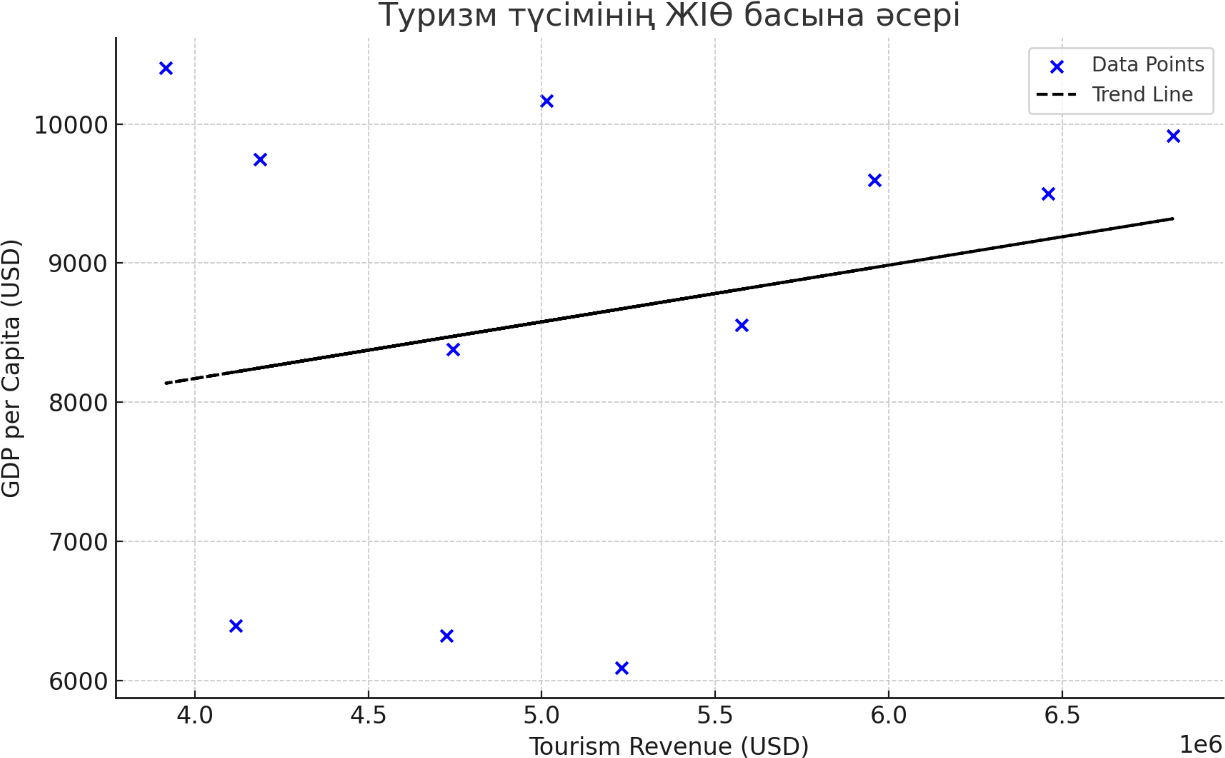
\includegraphics[width=0.8\textwidth]{assets/1114}
	\caption*{}
\end{figure}

{\bfseries 1-сурет - Туризмнен түскен табыс жан басына шаққандағы жалпы
ішкі өнімге әсері.}

{\bfseries Тренд сызығы оң қатынасты көрсетеді}

\begin{figure}[H]
	\centering
	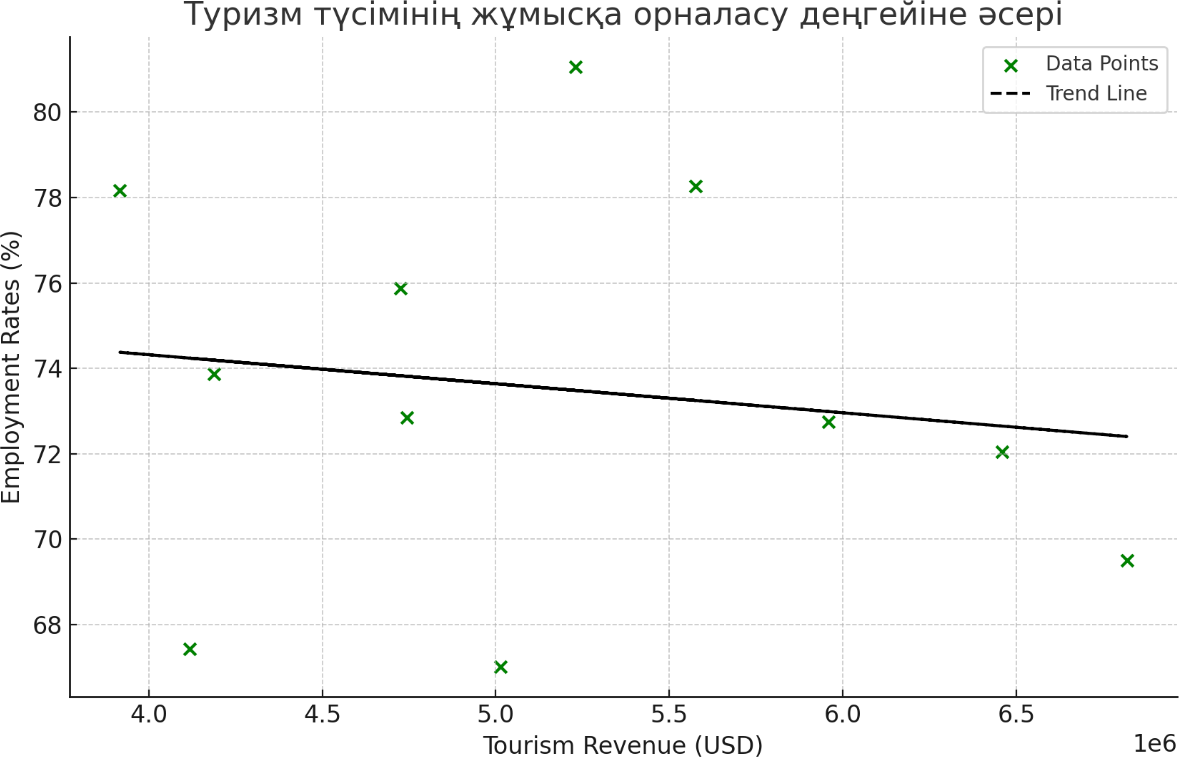
\includegraphics[width=0.8\textwidth]{assets/1115}
	\caption*{}
\end{figure}

{\bfseries 2-сурет - Туризмнен түскен табыс пен жұмыспен қамту деңгейі
арасындағы корреляцияны көрсетеді}

\begin{figure}[H]
	\centering
	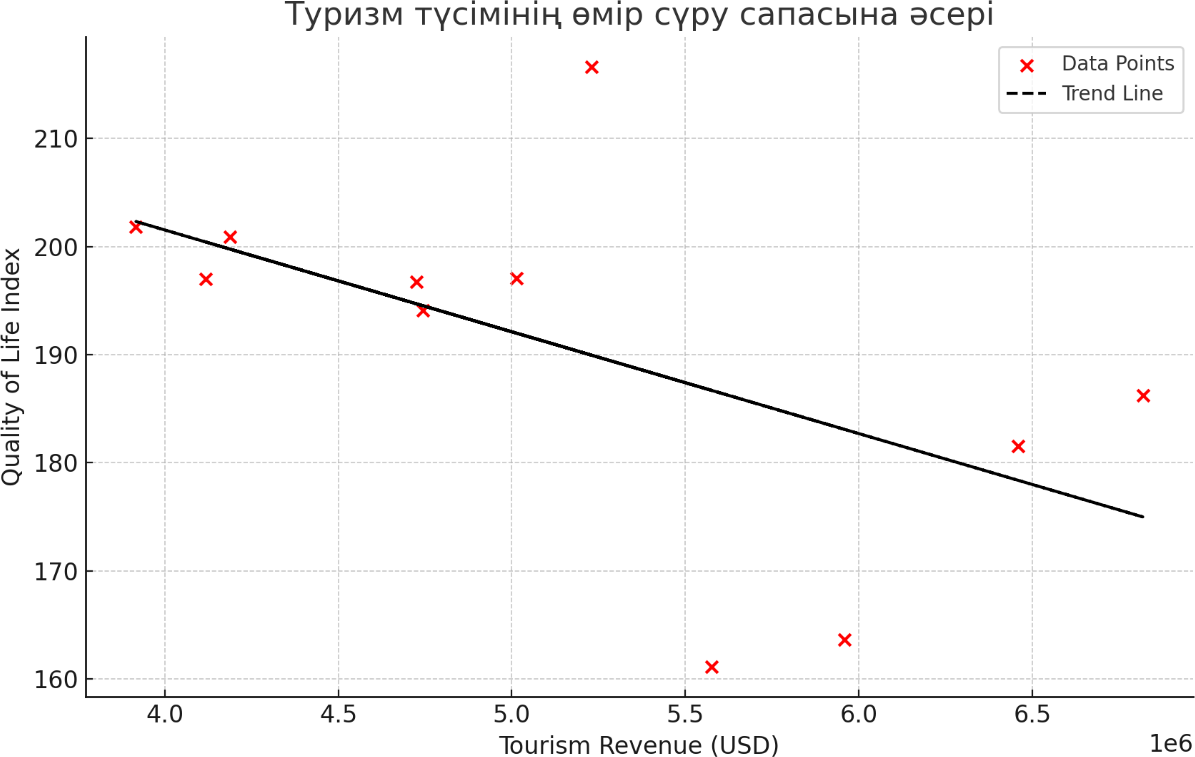
\includegraphics[width=0.8\textwidth]{assets/1116}
	\caption*{}
\end{figure}

{\bfseries 3-сурет - Туризм кірісінің артуы өмір сапасы индексін қалай
жақсартуы мүмкін екенін көрсетеді}

Нәтижелер туризмнен түскен табыс пен барлық үш тәуелді айнымалы
арасындағы оң және статистикалық маңызды қатынасты көрсетеді. Атап
айтқанда, туризмнен түсетін кірістің артуы жан басына шаққандағы ЖІӨ-нің
жоғарылауымен, жұмыспен қамту деңгейінің жақсаруымен және өмір сапасының
жақсаруымен байланысты.

Сұхбаттардың сапалы деректері осы тұжырымдарды толықтырады, бұл
туризмнің экономикалық тұрақтылықты нығайтып қана қоймай, сонымен қатар,
аймақтағы әлеуметтік және мәдени серпінділікке ықпал еткенін көрсетеді.

Зерттеу құнды түсініктер бергенімен, сыртқы жаһандық экономикалық
факторлардың, соның ішінде COVID-19 пандемиясының әсері сияқты
шектеулерді мойындайды. Туризмнің ұзақ мерзімді қоршаған ортаға әсерін
зерттеу және ағымдағы өсудің тұрақтылығын бағалау үшін қосымша
зерттеулер қажет.

Бұл зерттеу Солтүстік Қазақстанның әлеуметтік-экономикалық негізін
жақсартудағы туризмнің маңызды рөлін көрсетеді. Қорытындылар экологиялық
және әлеуметтік салдарларды ескере отырып, туризмнің пайдасын барынша
арттыруға бағытталған саяси шешімдерді басшылыққа алады деп күтілуде.

Қазіргі таңда Солтүстік Қазақстанның 2010-2020 жылдардағы деректерін
талдау туризмнен түскен кірістің өңір экономикасына, жұмыспен қамтуға
және өмір сүру сапасына оң әсерін айқын көрсетеді. Туризмнен түскен
табыстың артуымен жан басына шаққандағы ЖІӨ және жұмыспен қамту деңгейі
де өседі, бұл туризмнің жұмыс орындарын құруға ықпал ететін маңызды
экономикалық драйвер екенін көрсетеді. Сонымен қатар, өмір сапасы
көрсеткіштерінің жақсаруы туризмнің пайдасы экономикалық шаралардан,
инфрақұрылым мен мемлекеттік қызметтерді жақсартудан тыс екенін
көрсетеді.

Жергілікті мүдделі тараптармен жүргізілген сұхбаттар туризмнің артуына
байланысты қауымдастықтың инфрақұрылымы мен мәдени алмасудағы көрінетін
жақсартуларды атап көрсете отырып, осы тұжырымдарды растайды. Дегенмен,
зерттеу шектеулерді, соның ішінде деректерді бұрмалауы мүмкін COVID-19
пандемиясы сияқты жаһандық оқиғалардың әсерін мойындайды. Туризмнің ұзақ
мерзімді тұрақтылығын және оның қоршаған ортаға әсерін зерттеу үшін
болашақ зерттеулер ұсынылады.

Бұл зерттеу саясаткерлерге туризмді аймақтық дамудың стратегиялық
элементі ретінде пайдалану үшін негіз болып табылады, экономикалық пайда
мен тұрақтылықты теңестіреді.

{\bfseries Қорытынды.} Күрделі жүйелердің жұмыс істеу процесстерін қатаң
аналитикалық зерттеу тіпті де мүмкін емес. Олардың аналитикалық
моделдерін анықтау көптеген жағдайларға, жұмыс ерекшеліктеріне, оны
құрайтын бөліктердің өзара әрекеттеріне қара, қоршаған әсерлерге және
т.с.с байланысты қиын болып келеді. Зерттеу нәтижесінде туризмнен
түсетін табыс Солтүстік Қазақстанның әлеуметтік-экономикалық дамуына
айтарлықтай үлес қосатынын дәлелдеді. 2010 жылдан 2020 жылға дейінгі
деректерді талдайтын көп нұсқалы регрессиялық модель арқылы туристік
кірістің өсуі жан басына шаққандағы ЖІӨ-нің жоғарылауымен, жұмыспен
қамту деңгейінің жақсаруымен және өмір сапасының жақсаруымен оң
байланысты екені анық. Бұл тұжырымдар туризмнің экономикалық серпіліс
ретінде ғана емес, сонымен қатар, инфрақұрылымды дамыту мен кеңейтілген
мемлекеттік қызметтерді қоса алғанда, кең әлеуметтік игіліктер үшін
катализатор ретіндегі шешуші рөлін атап көрсетеді.

Оң нәтижелерге қарамастан, зерттеу өсу стимуляторы ретінде туризмнің
сенімділігіне әсер етуі мүмкін сыртқы экономикалық күйзеліс, әсіресе
COVID-19 пандемиясы сияқты ықтимал шектеулерді мойындайды. Осылайша,
туризмнің тікелей пайдасы анық болғанымен, оның ұзақ мерзімді
тұрақтылығы мен әсері, әсіресе қоршаған ортаға әсер ету және
экономикалық тұрақтылық салаларында қосымша зерттеулерді қажет етеді.

Осы тұжырымдарды ескере отырып, саясаткерлерге тек экономикалық өсуді
ғана емес, сонымен қатар, қоршаған орта мен мәдени құндылықтарды
сақтайтын тұрақты тәжірибеге басымдық беретін туризмге стратегиялық
инвестицияларды қарастыру ұсынылады. Бұл тәсіл Солтүстік Қазақстандағы
туризмнің гүлденген, жан-жақты және тұрақты болашаққа үлес қоса отырып,
дамудың сенімді драйвері болып қалуын қамтамасыз етеді.

{\bfseries Әдебиеттер}

1. Gössling S., Scott D., Hall C. M. Pandemics, tourism and global
change: a rapid assessment of COVID-19// Journal of Sustainable Tourism.
-2020. -Vol.29(1). -P. 1-20. DOI 10.1080/09669582.2020.1758708

2. Li Y., Hu C., Huang C., Duan, L. The concept of smart tourism in the
context of tourism information services// Tourism Management. -2019.
-Vol. 58. -P. 293-300. DOI 10.1016/j.tourman.2016.03.014

3.Sigala M. New technologies in tourism: From multi-disciplinary to
anti-disciplinary advances and trajectories// Tourism Management
Perspectives. -2018. -Vol. 25. - P. 151-155. DOI
10.1016/j.tmp.2017.12.003

4.Budeanu A., Miller G., Moscardo G., Ooi C. S. (2016). Sustainable
tourism, progress, challenges and opportunities: an introduction//
Journal of Cleaner Production. -2016. -Vol. 111. -P. 285-294. DOI
10.1016/j.jclepro.2015.10.027

5.Higgins-Desbiolles F. Socialising tourism for social and ecological
justice after COVID-19. //Tourism Geographies. -2018. -Vol. 22(3). - P.
610-623. DOI 10.1080/14616688.2020.1757748

6.Brida J. G., Cortes-Jimenez I., Pulina M. Has the tourism-led growth
hypothesis been validated? A literature review. //Current Issues in
Tourism. -2016. -Vol. 19(5). - P.394-430. DOI
10.1080/13683500.2013.868414

7.Butler R. W. The concept of a tourist area cycle of evolution:
Implications for management of resources// Canadian Geographer. -1980.
-Vol. 24(1). -P. 5-12. DOI 10.1111/j.1541-0064.1980.tb00970.x

8.Kazakhstan National Statistics Office. Annual Economic Report. -2021.
--URL: https://stat.gov.kz/en/region/sko/ (date of the application
21.02.2024)

9.Local Government of North Kazakhstan. Annual Infrastructure
Development Report. -2020. --URL:
https://www.gov.kz/memleket/entities/sko/activities/4973?lang=en. (date
of the application -- 21.02.2024)

10.Kazakhstan Department of Health and Education. Social Metrics Report.
-2019. --URL: https://www.gov.kz/memleket/entities/dsm?lang=en. (date of
the application 25.02.2024)

11.Ministry of Education and Science of the Republic of Kazakhstan.
Ethical Guidelines for Research. -2018. --URL:
https://www.gov.kz/memleket/entities/edu?lang=en. (date of the
application 26.02.2024)

12. SPSS-tі zhelіde tegіn paidalana alamyn ba?: REVIEWS. -URL:
https://reviews.tn/kk/wiki/can-i-use-spss-online-for-free/ (date of the
application -- 03.003.2024) {[}in Kazakh{]}

\emph{{\bfseries Авторлар туралы мәліметтер}}

Бидахмет Ж. -PhD, әл-Фараби атындағы Қазақ ұлттық университетінің доцент
м.а., Алматы, Қазақстан,

е-mail: bidakhmetzhanar@gmail.com;

Исаев А.Р.-әл-Фараби атындағы Қазақ ұлттық университетінің
магистранты,Алматы, Қазақстан, е-mail: aydarisaev@mail.ru

\emph{{\bfseries Infоrmatiоn abоut the authоrs}}

Zh. Bidakhmet -- PhD, аcting Associate professor Al-Farabi Kazakh
National University, Almaty, Kazakhstan,

е-mail: bidakhmetzhanar@gmail.com;

A. Issayev- graduate student at Al-Farabi Kazakh National University,
Almaty, Kazakhstan ,е-mail: aydarisaev@mail.ru\newpage
{\bfseries МРНТИ 06.73.45}

{\bfseries ДЕНЕЖНАЯ СИСТЕМА НЕЗАВИСИМОГО КАЗАХСТАНА: СТАНОВЛЕНИЕ И
НАПРАВЛЕНИЯ ДАЛЬНЕЙШЕГО РАЗВИТИЯ}

{\bfseries \textsuperscript{1}К.Ж.Садвокасова,
\textsuperscript{1}А.С.Бактымбет, \textsuperscript{2}Р.К.Садвокасов,}

{\bfseries \textsuperscript{1}А.К.Алпысбаева \textsuperscript{1}С.Рейдолда}

\textsuperscript{1}Казахский университет технологии и бизнеса, Астана,
Казахстан,

\textsuperscript{2}Евразийский национальный университет им.Л.Н.Гумилева,
Астана, Казахстан

Корреспондент-автор: ksadvokas@mail.ru

В 2023 году исполнилось~ровно~30 лет со дня принятия государственных
символов Республики Казахстан и 30 лет независимой денежной системе
Казахстана как суверенного государства. Уважение к Отчизне, трепетное
отношение к родной земле начинается с уважения к национальным
государственным символам, которые являются~~главными атрибутами
суверенитета страны, важнейшим инструментом укрепления национального
духа и общественного согласия, а также патриотического воспитания и
развития современной национальной экономики.~Таким же непременным
атрибутом суверенного государства является - независимая, устойчивая
денежная и финансовая система Республики Казахстан. Так как от состояния
денежной системы зависит успешное развитие национальной экономики.
Каждое суверенное государство имеет свою денежную систему. Под денежной
системой принято понимать форму организации денежного обращения в
стране, исторически сложившуюся и закрепленную национальным
законодательством. Составной частью денежной системы является
национальная валюта, которая в то же время относительно самостоятельна.
Денежные системы многих ныне развитых стран берут свое начало в
XVI--XVII веках, в период формирования национальных рынков и укрепления
государственной власти. Поэтому можно сказать, что современные денежные
системы различных стран имеют длительную историю, свои национальные
исторические и экономические особенности. В связи с этим фактором можно
сказать, что современный Казахстан сравнительно молодое государство. И
Казахстан не стал исключением по созданию своей независимой денежной
системы и не избежал ошибок, поскольку является довольно молодым
государством. Поэтому важно рассмотреть основные этапы становления и
развития независимой национальной денежной системы Казахстана.

{\bfseries Ключевые слова:} денежная система, элементы денежной системы,
национальная валюта, государство, финансовая система.

{\bfseries ТӘУЕЛСІЗ ҚАЗАҚСТАННЫҢ АҚША ЖҮЙЕСІ: ҚАЛЫПТАСУЫ}

{\bfseries ЖӘНЕ ОДАН ӘРІ ДАМУ БАҒЫТТАРЫ}

{\bfseries \textsuperscript{1}Қ. Ж. Сәдуақасова,
\textsuperscript{1}А.С.Бақтымбет, \textsuperscript{2}Р.К.Сәдуақасов,}

{\bfseries \textsuperscript{1}А.К.Алпысбаева,
\textsuperscript{1}С.Рейдолда}

\textsuperscript{1}Қазақ технология және бизнес университеті, Астана,
Қазақстан,

\textsuperscript{2} Л.Н.Гумилев атындағы Еуразия ұлттық университеті,
Астана, Қазақстан,

e-mail: ksadvokas@mail.ru

2023 жылы Қазақстан Республикасының Мемлекеттік рәміздерінің
қабылданғанына тура 30 жыл және Қазақстанның егемен мемлекет ретіндегі
тәуелсіз ақша жүйесіне 30 жыл толды. Отанға деген құрмет, туған жерге
деген құрмет елдің егемендігінің басты атрибуттары, ұлттық рух пен
қоғамдық келісімді нығайтудың, сондай-ақ қазіргі ұлттық экономиканы
патриоттық тәрбиелеу мен дамытудың маңызды құралы болып табылатын ұлттық
мемлекеттік рәміздерді құрметтеуден басталады. Қазақстан Республикасының
тәуелсіз, тұрақты ақша және қаржы жүйесі - егеменді мемлекеттің дәл
осындай ажырамас атрибуты болып табылады. Өйткені ұлттық экономиканың
табысты дамуы ақша жүйесінің жағдайына байланысты. Әрбір егеменді
мемлекеттің өзіндік ақша жүйесі бар. Ақша жүйесі деп тарихи қалыптасқан
және ұлттық заңнамамен бекітілген елдегі ақша айналымын ұйымдастыру
формасы түсініледі. Ақша жүйесінің ажырамас бөлігі-бұл салыстырмалы
түрде тәуелсіз ұлттық валюта. Көптеген дамыған елдердің ақша жүйелері
XVI--XVII ғасырларда, ұлттық нарықтардың қалыптасуы мен мемлекеттік
биліктің нығаюы кезеңінде пайда болды. Сондықтан әр түрлі елдердің
қазіргі ақша жүйелерінің ұзақ тарихы, ұлттық тарихи және экономикалық
ерекшеліктері бар деп айтуға болады. Осы факторға байланысты қазіргі
Қазақстан салыстырмалы түрде жас мемлекет деп айтуға болады. Қазақстан
өзінің тәуелсіз ақша жүйесін құруда да ерекшелік болған жоқ және
қателіктерден қашқан жоқ, өйткені ол өте жас мемлекет. Сондықтан
Қазақстанның тәуелсіз ұлттық ақша жүйесінің қалыптасуы мен дамуының
негізгі кезеңдерін қарастыру маңызды.

{\bfseries Түйін сөздер}: ақша жүйесі, ақша жүйесінің элементтері, ұлттық
валюта, мемлекет, қаржы жүйесі.

{\bfseries THE MONETARY SYSTEM OF INDEPENDENT KAZAKHSTAN:}

{\bfseries FORMATION AND DIRECTIONS OF FURTHER DEVELOPMENT}

{\bfseries \textsuperscript{1}K.J.Sadvokasova, \textsuperscript{1}A.S.
Baktymbet , \textsuperscript{2}R.K.Sadvokasov,}

{\bfseries \textsuperscript{1}A.K.Alpysbaeva, \textsuperscript{1}S.
Reidolda}

\textsuperscript{1} Kazakh University of Technology and Business,
Astana, Kazakhstan,

\textsuperscript{2} L.N.Gumilev Eurasian National University, Astana,
Kazakhstan,

e-mail: ksadvokas@mail.ru

In 2023, exactly 30 years have passed since the adoption of the state
symbols of the Republic of Kazakhstan and 30 years of the independent
monetary system of Kazakhstan as a sovereign state. Respect for the
Motherland, reverent attitude to the native land begins with respect for
national state symbols, which are the main attributes of the
country\textquotesingle s sovereignty, an important tool for
strengthening the national spirit and social harmony, as well as
patriotic education and the development of a modern national economy.
The same indispensable attribute of a sovereign state is an independent,
stable monetary and financial system of the Republic of Kazakhstan.
Since the successful development of the national economy depends on the
state of the monetary system. Each sovereign state has its own monetary
system. The monetary system is usually understood as a form of
organization of monetary circulation in the country, historically
established and enshrined in national legislation. An integral part of
the monetary system is the national currency, which at the same time is
relatively independent. The monetary systems of many now developed
countries originate in the XVI--XVII centuries, during the formation of
national markets and the strengthening of state power. Therefore, it can
be said that modern monetary systems of various countries have a long
history, their own national historical and economic characteristics. In
connection with this factor, we can say that modern Kazakhstan is a
relatively young state. And Kazakhstan was no exception in creating its
own independent monetary system and did not avoid mistakes, since it is
a fairly young state. Therefore, it is important to consider the main
stages of the formation and development of an independent national
monetary system in Kazakhstan.

{\bfseries Keywords}: monetary system, elements of the monetary system,
national currency, state, financial system.

{\bfseries Введение.} В этой связи необходимо рассмотреть становление
денежной системы Республики Казахстан, так как наше государство является
сравнительно молодым. А сам процесс становления денежной системы не
избежал ряд ошибок, трудностей и даже парадоксов. Как известно
элементами денежной системы являются следующее:

- национальная денежная единица;

- виды денежных знаков;

- масштаб цен;

- эмиссионный механизм.

Денежная система Республики Казахстан была построена на основе денежной
планово-командной экономики СССР. Поэтому денежная система Республики
Казахстан унаследовала все трудности и проблемы денежной системы
советского государства. Основной денежной единицей был советский рубль,
который имел золотое содержание 0, 987412 г. золота. В обращении
находились казначейские билеты Основой достоинством в 1, 3, 5 рублей и
банковские билеты достоинством в 10, 25, 50, 100 рублей и разменная
монета. Причем уже позже после развала СССР не советские рубли, а
российские рубли имели хождение на территории Республики Казахстан
вплоть до 15 ноября 1993 года -даты введения национальной валюты
«тенге», хотя как известно независимость наша страна обрела еще в 1991
году. Поэтому важно рассмотреть и проанализировать основные этапы
развития и совершенствования денежной системы Казахстана. Так как
политический суверенитет не означает еще экономический суверенитет.

{\bfseries Материалы и методы.} При написании статьи были использованы
следующие методы: методы сравнительного анализа, метод диалектического
материализма, эмпирические методы, сравнительно-исторический метод.

Цель исследования заключается в анализе основных этапов развития
национальной денежной системы Казахстана, как суверенного государства и
влияние на ее развитие не только экономических факторов, но и
политических. Всегда ли Национальный банк Казахстана принимал
своевременные и решительные меры по борьбе с инфляцией?

Гипотеза строится на том, что несмотря на заявления руководства
Казахстана, что проводим независимую экономическую политику, тем не
менее влияние внешних факторов сильно влияет на уровень инфляции в
стране и соответственно на состояние экономики.

Новизна данной статьи заключается в том, что до сих пор не были
исследованы причины инфляции на разных этапах развития рыночной
экономики и причины несвоевременного реагирования на эти процессы
главного банка страны -- Национального банка Республики Казахстан, как
проводника соотвествующей денежно-кредитной политики.

Как уже было сказано денежная система различных стран имеет свои
национальные и исторические особенности. Такие особенности имеет и
Республика Казахстана. К ним можно отнести следующие факты:

Во - первых, независимость Республики Казахстан была объявлена
16.12.1991 года. Однако мы не можем утверждать, что уже в 1991 году
Казахстан имел независимую самостоятельную денежную систему, так как на
этот период отсутствовали отдельные элементы денежной системы, а именно
- национальная единица денежного счета. Так как в обращении находилась
по сути дела валюта другого государства - российский рубль, эмитируемый
Центральным банком Российской Федерации.

Во - вторых, поскольку обращался российский рубль вплоть до 15 ноября
1993 года, то виды денежных знаков, выпускаемых, в обращении естественно
устанавливались не Национальным банком Республики Казахстан, а
Центральным банком Российской Федерации.

Поэтому можно сказать Республика Казахстан объявив последней из всех
республик СССР политическую независимость не был подлинно экономически
независимым государством

В - третьих, поскольку Национальный банк Республики Казахстан не
выпускал денег в обращении, то он не выполнял свою главную функцию-
эмиссионную. И это притом, что согласно Закону еще Казахской ССР с 1990
года, в нашем государстве функционировала двухуровневая банковская
система.

В - четвертых, отсутствовала полноценная законодательно - нормативная
база, так как Законы РК «О Нацбанке РК», и «О банках и банковской
деятельности» от 1993 года были не совершенны, поскольку были приняты
еще до введения национальной валюты. Также эти законы не полностью
отражали роль, функции и полномочия банков в рыночных отношениях.

В - пятых, надо отметить, что введение национальной валюты в Республике
Казахстан происходило в экстренном порядке. Так как, в августе 1993 года
правительство России в одностороннем порядке нарушило договор о едином
экономическом пространстве с единой валютой, введя в обращении денежные
знаки нового дизайна, которые имели хождение только на территории
Российской Федерации. Тем самым произошло фактическое разделение
денежных систем России и Казахстана. И день 15 ноября в Республики
Казахстан является днем национальной валюты и профессиональным
праздником работников финансовой, бюджетной, налоговой,
кредитно-банковской систем.

В - шестых, Закон РК «О денежной системе Республики Казахстан» был
принят только в декабре 1993 года. Этот закон устанавливает правовые
основы и формы организации денежного обращения, включающий в себя
официальную денежную единицу, порядок чеканки монет и эмиссии денежных
знаков. В данном законе говорится, что единственным законным платежным
средством на территории Республики Казахстан является -- тенге. Однако
нужно отметить, что на практике часто это положение нарушается, особенно
СМИ, где публикуются объявления о купле--продаже и цена товара, услуг
или недвижимости указывается в иностранной валюте.

В - седьмых, более совершенные Законы Республики Казахстан «О Нацбанке»
и «О банках и банковской деятельности» были приняты в 1995 году, где
Национальному банку Республики Казахстан придан соответствующий статус
главного Центрального банка и четко разграничены функции и операции БВУ.

В - восьмых, сам 1993 год в истории Казахстана ознаменовался как год
введения национальной валюты, то за тем следующий 1994 год -год
обвального падения национальной валюты тенге по отношению к доллару. На
момент введения национальной валюты 1 доллар США равнялся 4 тенге 65
тиын, а к концу 1994 года - почти 60 тенге. В 1994 году страна пережила
галопирующую, а затем гиперинфляцию и стагфляцию, сопровождавшуюся
спадом производства и ростом безработицы.

В - девятых, 1995 год -- год начала проведения Национальным банком
Республики Казахстан жесткой денежно-кредитной политики -«кредитной
рестрикции». Первые результаты были получены в 1996 году. 1996 год
переломный год в дальнейшем развитии денежной системы Республики
Казахстан, так как положено начало макроэкономической стабилизации.
Национальный банк Республики Казахстан становится подлинным центральным
банком нашего государства.

В - десятых, в 1999 году был введен свободный плавающий обменный
валютный курс, что явилось правильным решением, после известного
«черного августа» 1998 года в России. В Республике Казахстан создана
собственная банковская фабрика и монетный двор, которые полностью
обеспечивают потребности экономики в наличных деньгах. В последние годы
Национальный банк Республики Казахстан выпускает в обращение банкноты
нового дизайна. Ветхие деньги достоинством с 1 тенге до 50 тенге изъяты
из обращения и заменены металлическими монетами.

Большое значение Национальный банк Республики Казахстан придает монетной
продукции. Если в 1993 году были выпущены бумажные монеты, то сегодня
выпускаются монеты из различных сплавов, включая коллекционные и
инвестиционные, золотые и серебряные монеты, которые продаются по
рыночной цене\emph{.} Здесь уместно вспомнить, что первые подобные
монеты для Казахстана были изготовлены Австрийским монетным двором.
Первые бумажные деньги - тенге печатались в Англии и доставлялись
спецсамолетами в Казахстан {[}1{]}.

Опыт развитых стран, в частности США, говорит о том, что к созданию
независимой денежной системы каждая страна пришла через «свои» трудности
и проблемы. Любопытен тот факт, что еще в XVIII веке денежное обращение
на американском континенте обслуживалось иностранными деньгами -
английскими фунтами стерлингов и испанскими серебряными долларами. В
1785 году конгресс США объявил национальной денежной единицей - доллар.
Но денежное обращение в США было децентрализовано, банкноты выпускались
частными банками. К примеру, в 1859 году в обращении находились 5 400
видов банкнот, выпущенных более чем 1000 банками. И только в 1913 году
федеральным актом, была учреждена федеральная резервная система (ФРС),
которая включает 12 федеральных резервных банков. А доллар по сей день
является свободно конвертируемой валютой и выступает в роли мировых
денег. А многие страны ведут борьбу за дедолларизацию экономики, в том
числе и Казахстан.

Поэтому можно сказать, что за короткий период становления независимого
государства, Казахстан создал национальную денежную систему, а
банковская система Республики Казахстан была признана одной из лучших
среди стран СНГ. А Национальный банк Республики Казахстан подчинил свою
деятельность главной задаче - обеспечению устойчивости национальной
валюты и стабильности цен.

Однако надо сказать, что по истечении 30 лет независимости Казахстана
главный банк страны плохо справляется со своими главными функциями. За
что подвергся заслуженной критики со стороны Президента Республики
Казахстана Токаева К.К. в Послании от 1 сентября 2022 г. {[}2{]}.

Динамика девальвации тенге по отношению к доллару в период с 1993 года
по 2018 год приведена на рисунке 1{[}3{]}. Таким образом, если на момент
введения национальной валюты-тенге \$1 стоил 4,69 тенге. То на
1.11.2022г. \$1= 475 тенге. Инфляция составила 101,3 \%.

\begin{figure}[H]
	\centering
	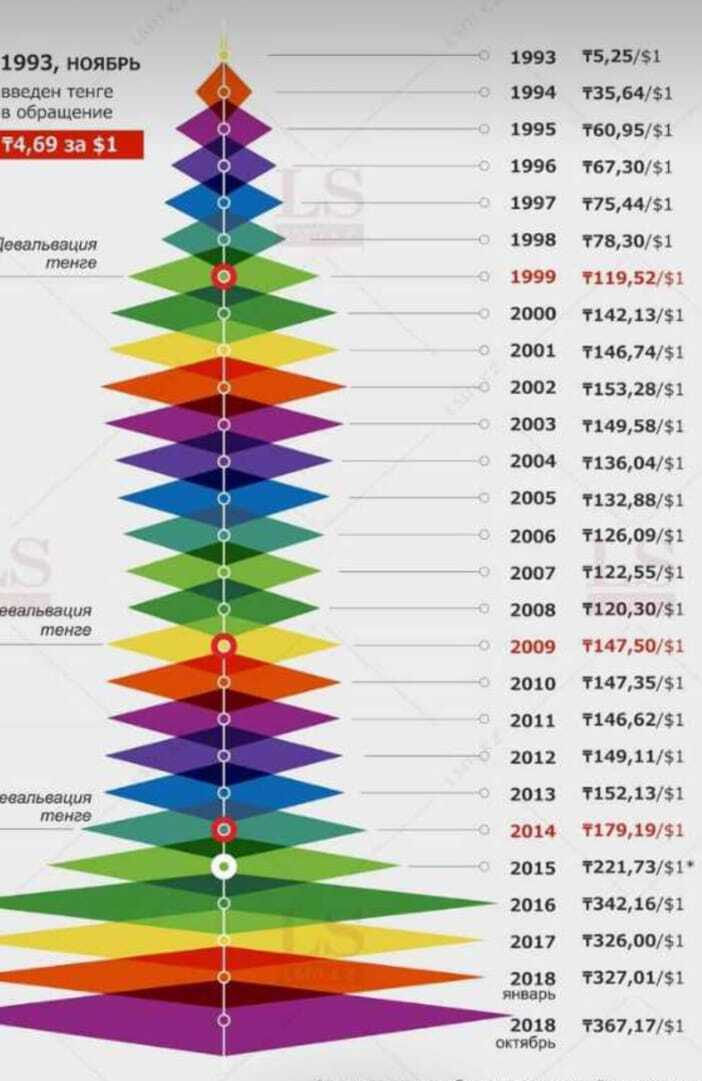
\includegraphics[width=0.8\textwidth]{assets/1117}
	\caption*{}
\end{figure}

{\bfseries Рис.1 - Динамика девальвации тенге за период с 1993 по 2018
годы}

{\bfseries Результаты обсуждения.} По итогам 2020 года, впервые за 10 лет
индустриализации, вклад обрабатывающей промышленности в развитие
экономики превысил долю горнодобывающей отрасли. Среднесрочная цель - к
2025 году увеличить экспорт обрабатывающей промышленности в 1,5 раза, до
24 млрд долларов, а производительность труда - на 30\% {[}2 {]}.

Вместе с тем, Президент Токаев К.К. подверг резкой критики деятельность
Национального банка Казахстан, который плохо справляется со своей
главной функцией денежно-кредитного регулирования экономики. Несмотря на
то, что Национальный Банк Казахстана самостоятельно, а также
взаимодействуя с другими государственными органами, разрабатывает и
осуществляет меры, направленные на обеспечение стабильности финансовой
системы:

1) проводит регулярный мониторинг макроэкономических и макрофинансовых
факторов, влияющих на стабильность финансовой системы;

2) формирует макропруденциальную политику;

3) предоставляет займы последней инстанции в порядке, предусмотренном
законодательством;

4) проводит мониторинг системных рисков финансовой системы;

5) в случае возникновения или угрозы возникновения системного
финансового кризиса

самостоятельно или совместно с Правительством Республики Казахстан
вводит ограничения на проведение отдельных видов банковских и других
операций финансовыми организациями.

Также им были отмечены, что Казахстан столкнулся с неконтролируемым
ростом инфляции. Национальный банк, Правительство Республики Казахстан
оказались бессильными перед ней, сославшись на мировые тенденции.
Подобного рода отговорки высвечивают уязвимость национальной экономики.
Возникает еще один вопрос: в чем тогда состоит роль наших
профессиональных экономистов? Главная задача Национального банка и
Правительства - это возвращение инфляции в коридор 4-6\% {[}2{]}.

Что касается инфляции, то по данным Бюро национальной статистики
Агентства по стратегическому планированию и реформам Республики
Казахстан, в августе 2021 года инфляция составила 0,5\% (в августе 2020
года -- 0,1\%). Годовая инфляция сложилась на уровне 8,7\% (в декабре
2020 года -- 7,5\%). В структуре инфляции цены на продовольственные
товары в годовом выражении повысились на 11,4\%, непродовольственные
товары -- на 7,3\%, платные услуги -- на 6,6\%. В августе 2021 года
количественная оценка ожидаемой через год инфляции по результатам опроса
населения составила 8,8{]}. Теперь о немонетарных составляющих инфляции.
Главная из них - цены на продукты питания.

\begin{figure}[H]
	\centering
	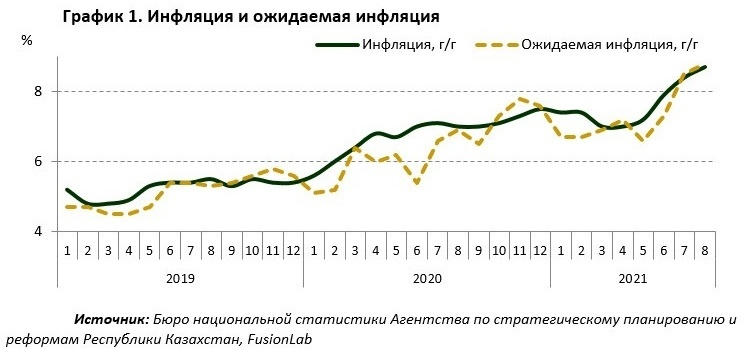
\includegraphics[width=0.8\textwidth]{assets/1118}
	\caption*{}
\end{figure}{\bfseries Рис.
2 -- Фактическая и ожидаемая инфляция в РК,}

{\bfseries в \%}

{\bfseries \_\_\_\_\_\_\_\_\_фактическая инфляция \_ \_ \_ \_ ожидаемая
инфляция}

Целью денежно-кредитной политики Национального Банка является удержание
инфляции в пределах установленных ориентиров. Среднесрочный таргет по
инфляции установлен на уровне 3-4\%. В целях обеспечения
сбалансированного экономического развития Национальный Банк стремится
осуществить постепенное снижение инфляции до данного уровня. Для этого
целевые ориентиры установлены следующим образом:

А) на 2021-2022 годы -- 4-6\%;

Б) на 2023-2024 годы -- 4-5\%;

В) с 2025 года -- 3-4\% {[}1 {]}.

\begin{figure}[H]
	\centering
	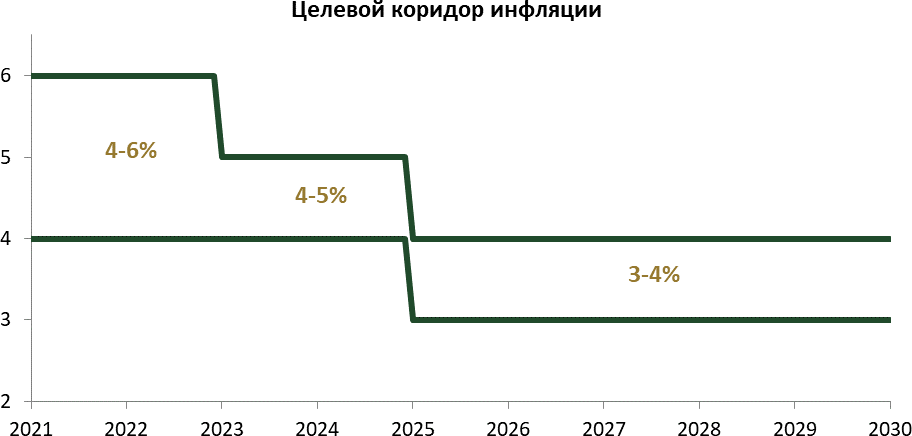
\includegraphics[width=0.8\textwidth]{assets/1119}
	\caption*{}
\end{figure}

{\bfseries Рис. 3 -- Целевые ориентиры по инфляции до 2025 года}

\emph{(Источник: данные сайта Нацбанка РК-www.nationalbank.kz)}

Однако эти целевые ориентиры по инфляции не были выдержаны по разным
причинам, в том числе из-за непредвиденных событий как начало СВО России
на Украине. За короткое время наша страна стала транзитной для беженцев
из России. Так россияне по данным Национального банка Казахстана завезли
в нашу страну около 50 млрд.рублей, которые подхлестнули цены на рынке
продовольствия, рынке недвижимости и рынке потребительских услуг и
соответственно инфляцию в стране, которая подскочила до 18\% в 2022 году
вместо планируемых 4-46\%.

В то же время на рынке труда продолжает расти число закрываемых
предприятий и число временно приостановленных, что говорит о
определенном кризисе в производственной сфере.

В~настоящее время в~Казахстане действуют почти 346,6 тыс. компаний.
В~их~число входят 172,2 тыс. активных юридических лиц (+1\% за~год),
53,8 тыс. вновь зарегистрированных (+11,9\%) и~120,6 тыс. временно
приостановленных (+16,5\%). Это следует из~данных бюро национальной
статистики.

Если рассматривать последнюю категорию предприятий, больше всего
временно приостановленных субъектов работали в~торговле, ремонте авто
и~мотоциклов (35,6 тыс.), в~строительстве (23 тыс.)
и~в~профессиональной, научной и~технической деятельности (7~729).

Также на~паузу поставили работу юридических лиц в~обрабатывающей
промышленности - в~сельском, лесном, рыбном хозяйстве, в~области
административного и~вспомогательного обслуживания, а~также транспорте
и~складировании. Помимо этого, в~Казахстане на~1~октября 2021 года
в~процессе ликвидации находится 5~421 предприятие {[}3{]}.

Это говорит о серьезном снижении роли банков в экономике. Достаточно для
этого сравнить показатели банков трех стран ЕАЭС -- Казахстана, России и
Беларуси. В результате реализации антикризисных мер общим объемом 6,3
трлн тенге в экономике возникла избыточная денежная масса. Но существуют
ниши, в которые эти средства не поступают. Банки второго уровня не
вкладываются в небольшие проекты, особенно на селе {[}4{]}.

В Казахстане и Российской Федерации процесс оптимизации
институциональной структуры продолжается. В частности, за период с 1
января 2013 года по 1 января 2020 года количество зарегистрированных и
имеющих право на осуществление банковских операций банков России
снизилось в два раза (с 923 до 402). За анализируемый период банковская
система Казахстана сократилась на 11 банков или почти на треть их общего
числа к уровню 2013 года, сохранив 27 банков второго уровня.

В целом, данный тренд соответствует глобальным тенденциям в сфере
финансового посредничества, которая находится под воздействием феномена
«цифровой компрессии». Индикаторами происходящих процессов являются не
только консолидация рынка, но и общее сокращение его объемов и
доходности бизнеса. Например, только в 2018 году в Европе прекратили
работу 330 банков или 5\% всего сегмента {[}5,6{]}.

Что же касается роли банковской системы в экономике, измеряемая как
отношение совокупных активов к ВВП, является индикатором эффективности
выполнения банками функции финансового посредника. В экономиках развитых
стран данный индикатор достигает размера ВВП. Надо отметить, что
банковский сектор России в данном случае является примером соответствия
лучшим мировым практикам, однако последние четыре года показатель
соотношения активов к ВВП также снижается (Таблица 2). Роль банковского
сектора Беларуси в финансировании экономики не только не достигает
порогового значения 60\% объёма ВВП, но имеет тенденцию к ежегодному
снижению.

Для Казахстана данное значение составляет менее 40\% и находится на
критическом уровне, что свидетельствует о недостаточности ресурсов и
наличии внутренних системных структурных рисков банковской системы, не
позволяющих банкам наращивать объёмы привлекаемых ресурсов для
вовлечения их в экономический оборот.

{\bfseries Таблица 1 -- Совокупные активы банковского сектора в \% к ВВП}

\begin{longtable}[]{@{}
  >{\raggedright\arraybackslash}p{(\columnwidth - 14\tabcolsep) * \real{0.1611}}
  >{\raggedright\arraybackslash}p{(\columnwidth - 14\tabcolsep) * \real{0.1162}}
  >{\raggedright\arraybackslash}p{(\columnwidth - 14\tabcolsep) * \real{0.1180}}
  >{\raggedright\arraybackslash}p{(\columnwidth - 14\tabcolsep) * \real{0.1180}}
  >{\raggedright\arraybackslash}p{(\columnwidth - 14\tabcolsep) * \real{0.1328}}
  >{\raggedright\arraybackslash}p{(\columnwidth - 14\tabcolsep) * \real{0.1180}}
  >{\raggedright\arraybackslash}p{(\columnwidth - 14\tabcolsep) * \real{0.1180}}
  >{\raggedright\arraybackslash}p{(\columnwidth - 14\tabcolsep) * \real{0.1180}}@{}}
\toprule\noalign{}
\begin{minipage}[b]{\linewidth}\raggedright
Страна
\end{minipage} & \begin{minipage}[b]{\linewidth}\raggedright
2014
\end{minipage} & \begin{minipage}[b]{\linewidth}\raggedright
2015
\end{minipage} & \begin{minipage}[b]{\linewidth}\raggedright
2016
\end{minipage} & \begin{minipage}[b]{\linewidth}\raggedright
2017
\end{minipage} & \begin{minipage}[b]{\linewidth}\raggedright
2018
\end{minipage} & \begin{minipage}[b]{\linewidth}\raggedright
2019
\end{minipage} & \begin{minipage}[b]{\linewidth}\raggedright
2020
\end{minipage} \\
\midrule\noalign{}
\endhead
\bottomrule\noalign{}
\endlastfoot
Казахстан & 45,1 & 46,3 & 61,4 & 57,6 & 45,4 & 40,8 & 39,6 \\
Беларусь & 54,9 & 55,2 & 64,5 & 67,2 & 58,4 & 53,9 & 54,6 \\
Россия & 80,9 & 99,6 & 102,7 & 93,01 & 92,5 & 90,2 & 88,3 \\
\multicolumn{8}{@{}l@{}}{%
Источник -- {[}4,5,6{]}} \\
\end{longtable}

Таким образом, можно сделать выводы, что в странах ЕАЭС есть
определенные трудности и несоответствие по ряду показателей, которые
нужно будет преодолеть в кратчайшие сроки, так как банковские системы
являются основным звеном финансового рынка{[}7,8,9{]}

{\bfseries Таблица 2 -- Казахстан в мировом рейтинге разведанных земных
богатств}

\begin{longtable}[]{@{}
  >{\raggedright\arraybackslash}p{(\columnwidth - 6\tabcolsep) * \real{0.0488}}
  >{\raggedright\arraybackslash}p{(\columnwidth - 6\tabcolsep) * \real{0.3849}}
  >{\raggedright\arraybackslash}p{(\columnwidth - 6\tabcolsep) * \real{0.2798}}
  >{\raggedright\arraybackslash}p{(\columnwidth - 6\tabcolsep) * \real{0.2865}}@{}}
\toprule\noalign{}
\multicolumn{2}{@{}>{\raggedright\arraybackslash}p{(\columnwidth - 6\tabcolsep) * \real{0.4337} + 2\tabcolsep}}{%
\begin{minipage}[b]{\linewidth}\raggedright
НАИМЕНОВАНИЕ
\end{minipage}} & \begin{minipage}[b]{\linewidth}\raggedright
ДОЛЯ В \%
\end{minipage} & \begin{minipage}[b]{\linewidth}\raggedright
МЕСТО В МИРЕ
\end{minipage} \\
\midrule\noalign{}
\endhead
\bottomrule\noalign{}
\endlastfoot
1 & СВИНЕЦ & 22\% & 1 \\
2 & ЦИНК & 15,2 & 1 \\
3 & УРАН & 18,9 & 2 \\
4 & ХРОМОВЫЕ РУДЫ & 37,6 & 1 \\
5 & БАРИТ & 47,2 & 1 \\
6 & УГОЛЬ & 3,1 & 6 \\
7 & НЕФТЬ & 3,2 & 6 \\
8 & {\bfseries ЗОЛОТО} & {\bfseries 2,7\%} & {\bfseries 8} \\
9 & {\bfseries СЕРЕБРО} & {\bfseries 16\%} & {\bfseries 2} \\
10 & МЕДЬ & 7,1 & 3 \\
11 & НИКЕЛЬ & 1,4 & 12 \\
12 & КОБАЛЬТ & 3,9 & 5 \\
13 & БОКСИТЫ & 1,4 & 10 \\
14 & ЖЕЛЕЗО & 6 & 5 \\
15 & МАРГАНЕЦ & 30 & 2 \\
16 & ФОСФОРИТЫ & 4,5 & 6 и т.д. \\
& По размеру территории

Казахстан занимает & & 9 место из 148 стран \\
& НАСЕЛЕНИЕ КАЗАХСТАНА & 0,25 & от всего населения земли \\
\multicolumn{4}{@{}>{\raggedright\arraybackslash}p{(\columnwidth - 6\tabcolsep) * \real{1.0000} + 6\tabcolsep}@{}}{%
\emph{Примечание:} по данным сайта Бюро национальной статистики
Агентства по стратегическому планированию и реформам Республики
Казахстан {[}Электронный ресурс{]}. - Режим
доступа:http//www.zakon/kz} \\
\end{longtable}

Из данных таблицы 2 видно, что мы очень богатая страна природными и
сырьевыми ресурсами и можем построить успешную рыночную экономику с
устойчивой денежной системой и национальной валютой {[}10,11{]}.

{\bfseries Выводы.} Завершение перехода на режим полноценного инфляционного
таргетирования позволит создать благоприятные условия для устойчивого
роста диверсифицированной экономики, включающие высокий уровень доверия
к проводимой денежно-кредитной политике и, как следствие, национальной
валюте, стабилизацию инфляционных ожиданий, а также сохранение
плавающего курсообразования, которое будет способствовать устойчивости
платежного баланса и поддержанию достаточного уровня международных
резервов.

Денежно-кредитная политика, как один из элементов макроэкономической
политики государства, будет служить, в первую очередь, целям поддержания
и повышения благосостояния населения. Она продолжит обеспечивать
устойчивое функционирование экономики, и достижение общеэкономических
целей страны. Наиболее важным приоритетом денежно-кредитной политики
будет оставаться обеспечение стабильности цен и сглаживание циклических
колебаний экономической активности через воздействие процентных ставок
на спрос. Стабильность цен будет достигаться не только через снижение
фактической инфляции, но также посредством стабилизации ее долгосрочной
динамики. Стабильная и низкая инфляция позволит сохранить стоимость
активов населения и компаний, а также снизить связанные с ней
общественные издержки. Второй значимой целью Национального Банка будет
обеспечение финансовой стабильности. При возникновении рисков для
финансовой системы денежно-кредитная политика будет направлена на
повышение ее устойчивости {[}12{]}.

{\bfseries Литература:}

1.Годовые отчёты Национального Банка РК за 2020-2022 годы //
https://nationalbank.kz/docid=31\&switch=russian.- Дата обращения
15.10.2023 г.

2.Послание Президента РК Токаева К.К. «Единство народа и системные
реформы - прочная основа процветания страны» от 1.09.2021 года
{[}Электронный ресурс{]}. - Режим доступа:http//www.zakon/kz- Дата
обращения 15.10.2023 г.

3.Бюро национальной статистики Агентства по стратегическому планированию
и реформам Республики Казахстан {[}Электронный ресурс{]}. - Режим
доступа:http//www.zakon/kz- Дата обращения 15.10.2023 г.

4.Банковский сектор Республики Беларусь {[}Электронный ресурс{]}. -
Режим доступа:http//www.nbrb.by- Дата обращения 15.10.2023 г.

5.Текущее состояние банковского сектора Республики Казахстан
{[}Электронный ресурс{]}. - Режим доступа:http//www.nationalbank.kz -
Дата обращения 15.10.2023 г.

6.Обзор банковского сектора Российской Федерации. {[}Электронный
ресурс{]}.- Режим доступа:http//www.cbr.ru- Дата обращения 01.11.2023 г.

7.Концепция развития финансового сектора Республики Казахстан до 2030
года: утв. постановлением Правительства Республики Казахстан 29 августа
2014, №954 // https://nationalbank.kz/?docid=382\&switch=russian.
25.12.2015.- Дата обращения 01.10.2023 г.

8.Sadvokassova К.Zh., Kodasheva G.S., Slyamova B.I. To the question of
transformation of banking activities in Kazakhstan into banking business
// Известия Национальной Академии наук Республики Казахстан. - 2018. -
№1(317). - C. 64-70.

9.Садвокасова К.Ж., Кодашева Г.С. Факторы, влияющие на развитие
банковской деятельности в Казахстане в условиях роста неопределённости
// Известия высших учебных заведений. Поволжский регион. Общественные
науки. -- 2017. -- №1(41). -- С. 167-176.

10.Парусимова Н.И., Садвокасова К.Ж., Кодашева Г.С. Банки Казахстана в
условиях экономической нестабильности // Интеллект. Инновации.
Инвестиции. -- 2016. -- №11. -- С. 60-66.

11.Садвокасова К.Ж. Влияние роста неопределенности на развитие
банковской деятельности в Казахстане: теория и практика:
Монография.-«ТОО Полиграфический центр «Индиго Принт», Астана,
2022.-156с.

12.Сратегия денежно-кредитной политики до 2030 г./Постановление Нацбанка
РК: http//www.nationalbank.kz- Дата обращения 03.12.2023

\begin{enumerate}
\def\labelenumi{\arabic{enumi}.}

\item
\end{enumerate}

{\bfseries References}

1.Godovye otchjoty Nacional\textquotesingle nogo Banka RK za 2020-2022
gody // https://nationalbank.kz/docid=31\&switch=russian.- Data
obrashhenija 15.10.2023 g.

2.Poslanie Prezidenta RK Tokaeva K.K. «Edinstvo naroda i sistemnye
reformy - prochnaja osnova procvetanija strany» ot 1.09.2021 goda
{[}Jelektronnyj resurs{]}. - Rezhim dostupa:http//www.zakon/kz- Data
obrashhenija 15.10.2023 g.

3.Bjuro nacional\textquotesingle noj statistiki Agentstva po
strategicheskomu planirovaniju i reformam Respubliki Kazahstan
{[}Jelektronnyj resurs{]}. - Rezhim dostupa:http//www.zakon/kz- Data
obrashhenija 15.10.2023 g.

4.Bankovskij sektor Respubliki Belarus\textquotesingle{} {[}Jelektronnyj
resurs{]}. - Rezhim dostupa:http//www.nbrb.by- Data obrashhenija
15.10.2023 g.

5.Tekushhee sostojanie bankovskogo sektora Respubliki Kazahstan
{[}Jelektronnyj resurs{]}. - Rezhim dostupa:http//www.nationalbank.kz -
Data obrashhenija 15.10.2023 g.

6.Obzor bankovskogo sektora Rossijskoj Federacii. {[}Jelektronnyj
resurs{]}.- Rezhim dostupa:http//www.cbr.ru- Data obrashhenija
01.11.2023 g.

7.Koncepcija razvitija finansovogo sektora Respubliki Kazahstan do 2030
goda: utv. postanovleniem Pravitel\textquotesingle stva Respubliki
Kazahstan 29 avgusta 2014, №954 //
https://nationalbank.kz/?docid=382\&switch=russian. 25.12.2015.- Data
obrashhenija 01.10.2023 g.

8. Sadvokassova К.Zh., Kodasheva G.S., Slyamova B.I. To the question of
transformation of banking activities in Kazakhstan into banking business
// Izvestiya National Academy of Sciences of the Republic of Kazakhstan.
- 2018. - №1(317). - C. 64-70

9. Sadvokasova K.Zh., Kodasheva G.S. Faktory, vlijajushhie na razvitie
bankovskoj dejatel\textquotesingle nosti v Kazahstane v uslovijah rosta
neopredeljonnosti // Izvestija vysshih uchebnyh zavedenij. Povolzhskij
region. Obshhestvennye nauki. -2017. - №1(41). - S. 167-176.

10. Parusimova N.I., Sadvokasova K.Zh., Kodasheva G.S. Banki Kazahstana
v uslovijah jekonomicheskoj nestabil\textquotesingle nosti // Intellekt.
Innovacii. Investicii. -2016. - №11.- S. 60-66.

11.Sadvokasova K.Zh. Vlijanie rosta neopredelennosti na razvitie
bankovskoj dejatel\textquotesingle nosti v Kazahstane: teorija i
praktika: Monografija.-«TOO Poligraficheskij centr «Indigo Print»,
Astana, 2022.-156s.

12.Srategija denezhno-kreditnoj politiki do 2030 g./Postanovlenie
Nacbanka RK: http//www.nationalbank.kz- Data obrashhenija 03.12.2023

\emph{{\bfseries Сведения об авторах}}

Садвокасова К.Ж.- доктор экономических наук, профессор Казахского
университета технологии и бизнеса им. К.Кулажанова, Астана, Казахстан,
e-mail: ksadvokas@mail.ru;

Бактымбет А.С. -кандидат экономических наук, ассоциированный
профессор,Казахского университета

технологии и бизнеса им. К.Кулажанова, Астана, Казахстан,
e-mail:asem\_abs@mail.ru;

Садвокасов Р.К.- магистр экономических наук, главный специалист
Евразийского национального университета им. Л.Н. Гумилева, Астана,
Казахстан, e-mail:rustems@ mail.ru;

Алпысбаева А.К.- кандидат экономических наук, ассоциированный профессор
Казахского университета технологии и бизнеса им.К. Кулажанова, e-mail:
alpysbayeva.ainur77@mai.ru;

Рейдолда С. -магистр экономических наук, старший преподаватель
Казахского университета технологии и бизнеса им. К.Кулажанова, e-mail:
sau\_1981@mail.ru

{\bfseries Information about the author}

Sadvokasova K.Zh. - Doctor of Economics, Professor of Kazakh University
of Technology and Business named after K.Kulazhanov, Astana, Kazakhstan,
e-mail: ksadvokas@mail.ru;

Baktymbet A.S. - Candidate of Economic Sciences, Associate Professor, of
the Kazakh University of Technology and Business named after
K.Kulazhanov, Astana, Kazakhstan, e-mail:asem\_abs@mail.ru;

Sadvokasov R.K. - Master of Economic Sciences, Chief Specialist of L.N.
Gumilev Eurasian National University, Astana, Kazakhstan,
e-mail:rustems@ mail.ru;

Alpysbaeva A.K.- Candidate of Economic Sciences, Associate Professor of
Kazakh University of Technology and Business named after K.Kulazhanov,
Astana, Kazakhstan, e-mail: ,alpysbayeva.ainur77@mail.ru;

Reidolda S. - magistr ekonomicheskikh nauk, senior teacher of Kazakh
University of Technology and Business named after K.Kulazhanov, Astana,
Kazakhstan, e-mail: sau\_1981@mail.ru\newpage
{\bfseries МРНТИ 06.56.02}

{\bfseries APPROACHES TO MEASURING THE CREATIVE ECONOMY AND TRENDS IN THE
DEVELOPMENT OF THE IT SECTOR: THE IMPACT OF DIGITAL TECHNOLOGIES ON
CREATIVE INDUSTRIES}

{\bfseries \textsuperscript{1}A. Serikkyzy, \textsuperscript{1}A.B.
Akhmetova., \textsuperscript{2}S.E. Zhamalidenov}

\textsuperscript{1}Almaty Management University, Almaty, Kazakhstan,

\textsuperscript{2}Satbayev University, Almaty, Kazakhstan,

Correspondent-author: a.serikkyzy@almau.edu.kz

Today, the creative economy is often referred to a the new oil.
According to UN estimates, creative industries generate around 30
million jobs annually, contributing \$2.25 trillion to the global GDP.
Projections indicate that by 2030, the global creative
industry\textquotesingle s turnover will increase by an additional 40\%.
This sector creates high-income jobs, especially for talented youth.

In Kazakhstan, investments in the creative industry have increased more
than fourfold over the past decade. Currently, 3.5\% of the
country\textquotesingle s total employed population, or 310 thousand
people, work in this sector, contributing 2.7\% to the economy. To
unlock this sector\textquotesingle s potential, the government is
developing the Concept for the Development of Creative Industries for
2021-2025, establishing a unified vision for growth.

The concept of creative industries varies across countries, lacking a
universally accepted definition. Reports like
Australia\textquotesingle s "Creative Nation" (1994) and the
UK\textquotesingle s "Creative Industries Mapping Document" (1998) have
significantly influenced global perspectives. The UN recommends a
classification into four aggregated blocks, but terminology differs
across organizations, with UNESCO using "creative industries" and the EU
referring to "cultural and creative industries."

Creative industries encompass sectors built on creativity, intellectual
property, and technology. Definitions differ, but common sectors include
design, art, fashion, and more. Measuring the creative economy involves
various approaches, such as industry assessment, employment analysis,
and trade in creative goods and services. The "creative trident" concept
evaluates employment in specialists, supporting roles, and integrated
positions.

{\bfseries Keywords}: creative economy, creative industry, investments,
employment, global GDP, technology.

{\bfseries ШЫҒАРМАШЫЛЫҚ ЭКОНОМИКАНЫ ӨЛШЕУ ТӘСІЛДЕРІ ЖӘНЕ IT СЕКТОРЫНЫҢ ДАМУ
ТРЕНДЕНЦИЯЛАРЫ: ЦИФРЛЫҚ ТЕХНОЛОГИЯЛАРДЫҢ ШЫҒАРМАШЫЛЫҚ САЛАЛАРҒА ӘСЕРІ}

{\bfseries \textsuperscript{1}А. Серікқызы, \textsuperscript{1}А.Б.
Ахметова, \textsuperscript{2}С.Е. Жамалиденов}

\textsuperscript{1}Алматы Менеджмент Университеті, Алматы, Қазақстан,

\textsuperscript{2}Satbayev University, Алматы, Қазақстан,

e-mail: a.serikkyzy@almau.edu.kz

Бүгінде жасампаз экономиканы жаңа мұнай деп атайды. Біріккен Ұлттар
Ұйымының бағалауы бойынша, креативті салалар жыл сайын шамамен 30
миллион жұмыс орнын құрып, жаһандық ЖІӨ-ге 2,25 триллион доллар қосады.
Болжамдар 2030 жылға қарай жаһандық креативті индустрияның айналымы тағы
40\%-ға өсетінін көрсетіп отыр. Бұл секторда, әсіресе, талантты жастар
үшін жоғары жалақысы бар жұмыс орындары ашылады.

Қазақстанда шығармашылық индустрияға салынған инвестиция соңғы
онжылдықта төрт еседен астам өсті. Қазіргі уақытта елдегі жалпы жұмыспен
қамтылған халықтың 3,5 пайызы немесе 310 мың адам экономиканың 2,7
пайызын құрайтын осы салада жұмыс істейді. Осы сектордың әлеуетін ашу
үшін үкімет бірыңғай өсу стратегиясын белгілей отырып, 2021-2025
жылдарға арналған Шығармашылық индустрияны дамытудың негізін әзірлеуде.

Шығармашылық индустрия түсінігі әр елде әртүрлі және жаһандық деңгейде
қабылданған анықтамасы жоқ. Австралияның Шығармашылық ұлты (1994) және
Ұлыбританияның Шығармашылық индустрияларды картаға түсіру құжаты (1998)
сияқты есептер жаһандық перспективаларға айтарлықтай әсер етті. БҰҰ төрт
жиынтыққа жіктеуді ұсынады, бірақ терминология ұйымдар арасында
ерекшеленеді, ЮНЕСКО «шығармашылық индустрияларды» пайдаланады, ал ЕО
«мәдени және шығармашылық салаларға» сілтеме жасайды.

Шығармашылық салалар шығармашылыққа, зияткерлік меншікке және
технологияға негізделген секторларды қамтиды. Анықтамалар әртүрлі, бірақ
жалпы секторларға дизайн, өнер, сән және т.б. кіреді. Шығармашылық
экономиканы өлшеу саланы бағалау, жұмыспен қамтуды талдау және
шығармашылық тауарлар мен қызметтердің саудасы сияқты әртүрлі тәсілдерді
қамтиды. Creative Trident тұжырымдамасы мамандардың жұмысқа орналасуын,
көмекші рөлдерді және біріктірілген позицияларды бағалайды.

{\bfseries Түйін сөздер}: креативті экономика, креативті индустрия,
инвестиция, жұмыспен қамту, жаһандық ЖІӨ, технология.

{\bfseries ПОДХОДЫ К ИЗМЕРЕНИЮ КРЕАТИВНОЙ ЭКОНОМИКИ И ТЕНДЕНЦИИ В РАЗВИТИИ
ИТ-СЕКТОРА: ВЛИЯНИЕ ЦИФРОВЫХ ТЕХНОЛОГИЙ НА КРЕАТИВНЫЕ ИНДУСТРИИ}

{\bfseries \textsuperscript{1}А. Серікқызы, \textsuperscript{1}А.Б.
Ахметова, \textsuperscript{2}С.Е. Жамалиденов}

\textsuperscript{1}Алматы Менеджмент Университеті, Алматы, Қазақстан,

\textsuperscript{2}Satbayev University, Алматы, Казахстан,

e-mail: a.serikkyzy@almau.edu.kz

Сегодня креативная экономика часто называется новой нефтью. По оценкам
ООН, креативные отрасли ежегодно создают около 30 миллионов рабочих
мест, внося 2,25 триллиона долларов в мировой ВВП. Прогнозы показывают,
что к 2030 году оборот мировой креативной индустрии увеличится еще на
40\%. Этот сектор создает высокооплачиваемые рабочие места, особенно для
талантливой молодежи.

В Казахстане инвестиции в креативную индустрию выросли более
четырехкратно за последнее десятилетие. В настоящее время в этом секторе
работает 3,5\% от общего числа занятого населения страны, или 310 тысяч
человек, что составляет 2,7\% экономики. Чтобы разблокировать потенциал
этого сектора, правительство разрабатывает Концепцию развития креативных
индустрий на 2021--2025 годы, устанавливая единую стратегию роста.

Концепция креативных индустрий различается в разных странах и не имеет
всемирно признанного определения. Доклады, такие как "Creative Nation"
(1994) Австралии и "Creative Industries Mapping Document" (1998)
Великобритании, значительно повлияли на глобальные перспективы. ООН
рекомендует классификацию на четыре агрегированных блока, но
терминология отличается в различных организациях, с ЮНЕСКО, использующей
"креативные индустрии", а ЕС ссылается на "культурные и креативные
индустрии".

Креативные отрасли охватывают сектора, основанные на творчестве,
интеллектуальной собственности и технологиях. Определения различаются,
но общими секторами являются дизайн, искусство, мода и другие. Измерение
креативной экономики включает различные подходы, такие как оценка
отрасли, анализ занятости и торговля творческими товарами и услугами.
Концепция "креативного трезубца" оценивает занятость специалистов,
поддерживающих ролей и интегрированных позиций.

{\bfseries Ключевые слова}: креативная экономика, креативная индустрия,
инвестиции, занятость, мировой ВВП, технологии.

{\bfseries Introduction.} The concept of creative industries is directly
related to national specificity and varies in each individual country.
There is no universally applied understanding of creative industries
worldwide. Let\textquotesingle s compare the approaches to defining
creative industries that have emerged in different countries. In 1994,
Australia published a report titled "Creative Nation: Cultural Policy of
the Australian Government" (Department of Communications and the Arts
(Australia), 1994). In 1998, the UK Department for Culture, Media and
Sport (DCMS) released the "Creative Industries Mapping Document," the
first major report dedicated to measuring the impact of creative sectors
on the British economy, providing a definition for 13 sectors of
creative industries. This classification significantly influenced the
international economic landscape, drawing attention from policymakers,
and governments embarked on studying the contribution of creativity to
their economies.

The statistical tables of economic indicators for creative industries
published by DCMS include data from all creative sectors, assessing
their contribution to the gross value added of the UK economy. They
consist of three main sections: "Employment," "Gross Value Added," and
"Export Services." The creative industries in these tables are
categorized into the following groups:

- Advertising and marketing;

- Architecture;

- Crafts;

- Design, graphic design, and fashion;

- Film, television, video, broadcasting, and photography;

- Information technology, software, and computer services;

- Publishing;

- Museums, galleries, and libraries;

- Music, performing, and visual arts;

- Video game industry.

The United Nations recommends a classification into four main aggregated
blocks of creative industries, a classification also followed by UNIDO.
Among creative industries are:

- Industries based on the use of historical and cultural heritage (folk
arts and crafts, museum activities);

- Industries based on the arts (theater, music, painting, gallery
activities, etc.);

- Modern media and digital content production (film, video, audio,
animation production, data processing, software development, virtual and
augmented reality, computer and video games, blogging, mass media,
advertising, etc.);

- Applied creative industries (architecture, industrial design, fashion
industry, jewelry making, culinary industry, etc.).

Nevertheless, in international practice, there is no unified definition
and agreed-upon classification of creative industries. UNESCO experts
use the term "creative industries," while at the European Union level,
the term "cultural and creative industries" is applied, and the World
Intellectual Property Organization (WIPO) uses the term "copyright
industries." In some countries, they are still referred to as cultural
industries, while in the Republic of Korea and Japan, they are termed
the content industry. Hence, there are differences in approaches to
measuring and economically assessing creative industries in various
countries, and in some states, such as China, even at the regional and
city levels.

The development of the IT industry in Kazakhstan has seen significant
achievements in recent years, driven by substantial changes and
progress. Kazakhstan aspires to become a technological leader in Central
Asia, and to support this goal, the government has undertaken
initiatives to foster the growth of the IT sector. One such initiative
is the State Program "Digital Kazakhstan", approved by the Government of
the Republic of Kazakhstan on December 12, 2017, through Resolution No.
827 {[}1{]}. In the medium term, the program aims to accelerate economic
development and improve the quality of life through the utilization of
digital technologies, while in the long term, it seeks to create
conditions for transitioning to a digital economy.

The key directions of the State Program "Digital Kazakhstan" include the
development of a creative society and the creation of up to 110,000 new
jobs, transitioning to a proactive state with 80\% of government
services moved online, and implementing digital transformations in
various economic sectors, aiming for up to 5.9\% productivity growth.
The program also envisions the realization of a digital Silk Road to
increase internet users with a coverage of 81.5\% of the population.

In the international Digital Intelligence Index, Kazakhstan ranks 55th
in terms of digitization and 20th in the pace of digitization among 90
countries. In the World Digital Competitiveness Ranking, evaluating the
ability and readiness to implement digital technologies as a key factor
in economic transformations in business, government, and society,
Kazakhstan holds the 36th position out of 63 countries.

As of 2021, the share of the information and communication technology
(ICT) industry in Kazakhstan\textquotesingle s GDP stood at 3.3\%,
according to the Ministry of Digital Development, Innovation, and
Aerospace Industry of the Republic of Kazakhstan (MDDIA). In 2017, this
share was only 1.3\%, and further growth is anticipated by 2023.
According to the National Statistics Bureau, the market volume of
information technology in the ICT industry in Kazakhstan for the first
half of 2021 amounted to 435.66 billion tenge. IT services exceeded IT
equipment by more than twice, reaching 287.46 billion tenge. The IT
services sector is growing in the structure of
Kazakhstan\textquotesingle s IT market, constituting 66.8\%. When
assessing countries with developed digital economies based on the share
of ICT exports in the total volume of goods exports, Kazakhstan lags.
The volume of IT service exports as a percentage of the total export
volume of Kazakhstan in 2022 was 0.1\%. Nevertheless, Kazakhstan has the
potential for development, with a significant internet audience of 17.73
million users, representing 90.9\% of the population. This makes
Kazakhstan an attractive platform for the entry of major international
IT players, providing a new impetus for industry development.

{\bfseries Materials and methods.} The methodological foundation for the
quantitative measurement of creative industries and the creative economy
worldwide has not been definitively established. One of the initial
attempts to classify creative industries was undertaken by the
Department for Culture, Media, and Sport of the United Kingdom in 1998.
Later, UNESCO and UNCTAD proposed alternative typologies {[}2{]}. In
Europe and Asia, creative industries are grouped differently.

One of the current and most debated issues is the measurement of the
creative economy. Attempts to assess the scale of creative industries
and their impact on the national economy are undertaken in many
countries. The most used approaches include:

1. Sectoral Approach: This involves evaluating key economic indicators
based on aggregated groupings of types of economic activities, known as
creative industries.

2. Employment Assessment: This approach involves evaluating employment
based on groupings of professions related to the category of creative
professions.

3. Analysis of External Trade: This entails analyzing international
trade in creative goods and services using relevant statistical
groupings of goods and services, known as creative goods and services.

\begin{figure}[H]
	\centering
	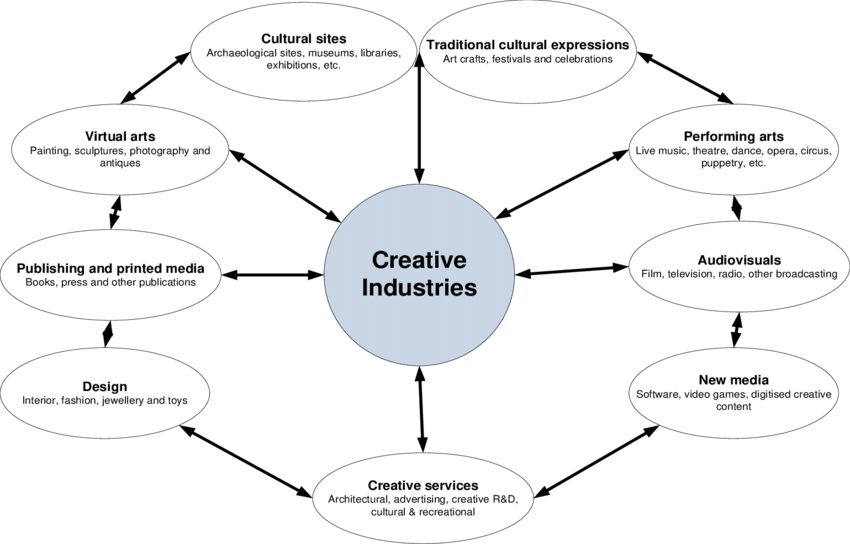
\includegraphics[width=0.8\textwidth]{assets/1120}
	\caption*{}
\end{figure}

{\bfseries Fig. 1 - UNCTAD Classification of Creative Goods {[}2{]}.}

The creative industries sector has the potential to create high added
value, making it attractive for both entrepreneurs and investors. Many
segments within this sector have relatively low market entry barriers,
providing an opportunity for a broad range of the population to develop
their businesses. This inclusivity extends to women, individuals with
disabilities, people residing in rural areas, and those in small towns,
allowing for widespread participation in the sector\textquotesingle s
growth.

Creative industries make a significant contribution to the global
economy. Over the period from 2002 to 2018, the average share of the
creative industries sector in the world GDP is 6.6\%. In developed
countries, this share reaches 8-12\%, with an average annual growth rate
of 15\%, substantially surpassing the average growth rates of the global
economy.

The creative industries make a substantial contribution to the global
economy. Over the period from 2002 to 2018, the sector has demonstrated
higher growth compared to other industries, generating around 3\% of the
world GDP and providing employment for 1\% of the global working
population. The development of creative industries brings multiple
positive effects to both the economy and society, including the growth
of small and medium-sized enterprises, job creation, diversification,
and an increase in non-commodity exports. It also contributes to
enhancing human capital quality by attracting talents and fostering
in-demand skills. Creative industries serve as a source of sustainable
inclusive growth, providing opportunities for self-development and
creating a conducive environment for living.

The creative economy presents a tangible development option for all
countries, particularly for developing nations. Additional data and
innovative interdisciplinary policy measures are needed to amplify the
impact of the creative sector on development.

The International Year of Creative Economy for Sustainable Development
in 2021 highlights the creative economy at a time when creative
solutions are essential for addressing global challenges {[}3{]}. As
emphasized in UN General Assembly Resolution 74/198 {[}4{]}, the
creative economy contributes comprehensively to achieving Sustainable
Development Goals (SDGs), especially Goals 1 (poverty eradication), 5
(gender equality), 8 (decent work and economic growth), 9 (industry,
innovation, and infrastructure), 10 (reduced inequality), 11
(sustainable cities), 12 (responsible consumption and production), 16
(peaceful and inclusive societies), and 17 (partnerships for the goals).

Cultural and creative industries undeniably make a significant
contribution to the global economy. The cultural sector accounts for
3.1\% of the world\textquotesingle s Gross Domestic Product (GDP), while
creative goods and services comprised 3\% and 21\%, respectively, of the
total volume of goods and services exports in 2020, according to UNCTAD
estimates {[}5{]}. Additionally, cultural, and creative industries
provide 6.2\% of all jobs worldwide, nearly 50 million, with a higher
representation of young people (15--29 years) compared to other sectors.
The creative economy promotes social inclusion, cultural diversity, and
human development. For these reasons, creative industries are crucial
for achieving the 2030 agenda. However, the COVID-19 pandemic has had a
devastating impact on some creative sectors, exacerbating longstanding
factors contributing to their vulnerability. A UNCTAD report indicates
that during this period, up to 10 million jobs disappeared in the
cultural and creative sectors, and in 2020, global production in these
sectors decreased by USD 750 billion {[}2{]}.

{\bfseries Results and discussion}.Analyzing the key aspects of the IT
industry in Kazakhstan, several development trends can be highlighted:

1. Economic Growth and Investments. In Kazakhstan, a favorable
environment has been established for investments in the IT sector. The
government actively supports startups and technology companies by
providing tax incentives and other stimuli. This approach attracts both
local and foreign investments into the markets. According to the
National Statistics Bureau of the Agency of Statistics of the Republic
of Kazakhstan, the IT market volume in 2022 amounted to 1.71 million
dollars, with a growth of 40.3\% in the ICT industry. The sector employs
69.5 thousand workers. The total capitalization of foreign technological
giants that relocated to Kazakhstan in 2022 reached 27 billion dollars
{[}6{]}. In 2020, the export of ICT goods and services amounted to
approximately 73.6 million US dollars, with ICT services contributing
more than 24 million US dollars. Over 50\% of service exports are
directed to European countries and the United States.

2. Training and Skill Development Programs. The development of the IT
industry in Kazakhstan involves the creation of educational programs and
courses focusing on software development, data analysis, and other
IT-related fields. The majority of IT specialists still receive
traditional education, completing bachelor\textquotesingle s and
master\textquotesingle s degrees. Currently, 84 out of 116 higher
education institutions provide training for information technology
professionals. Annually, 8,000 to 9,000 educational grants are allocated
for the preparation of IT specialists. The number of graduates from 2018
to 2020 reached 30,604. However, according to experts and market
participants, not more than 30\% of graduates possess the necessary
skills for a successful career in their field, as indicated by the
National Chamber of Entrepreneurs "Atameken" rating {[}7{]}.

Кazakhstan universities and training centers provide opportunities for
education and skills enhancement in the IT field. According to a survey
conducted by Kolesa Group {[}8{]}, 78\% of respondents studied IT
specialties at three major universities in the country -- International
IT University (17\%), SDU University (10\%), and Almaty University of
Power Engineering and Telecommunications (7\%).

The most in-demand IT specialists in Kazakhstan are:

1. Programmer, Developer.

2. Designer.

3.Analyst.

4. System Administrator.

5. Technical Support Specialist.

6. Information Security Specialist.

7. Systems Engineer.

8. Tester.

9. Network Engineer.

10. Game Designer.

Around 21\% of IT specialists in Kazakhstan officially work for at least
two companies. Since 2021, there has been a trend towards obtaining
education not only in universities but also through specialized
programs, allowing individuals to acquire specific skills and enhance
hard skills in a short period. For instance, in 2022, Tech Orda from
Astana Hub graduated 3,000 individuals, and alem.school trained 250
specialists through educational IT programs. The International Financial
Center "Astana" and Qwazar jointly launched the QWANT programming
school, currently educating 250 Kazakhstani and international
specialists.

According to digitalbusiness.kz {[}9{]}, the IT sector ranked fifth in
the rating of open job vacancies in Kazakhstan. In Q1 and Q2 of 2023,
more than 50,000 residents of Kazakhstan were searching for jobs in the
information technology sector. In 2022, about 40,000 IT job vacancies
were published, constituting 48\% of all job postings, according to the
hh.kz platform.

The high interest in IT specialties in Kazakhstan is driven by
competitive salaries in the IT sector, company bonuses, the development
of artificial intelligence, and the emergence of new innovative products
in the IT industry. According to hh.kz data, the salary for a leading
DevOps engineer and Java- and iOS-developers varies from 700,000 to 2.3
million tenge, with the average salary for an IT specialist in 2022
reaching 515,600 tenge {[}8{]}.

3. Startup Ecosystem. The startup ecosystems in Kazakhstan are actively
evolving. Incubators, accelerators, and technoparks have been
established to foster the digital sector and support young
entrepreneurs, contributing to the development of innovations and new
technological projects. Some of the largest ones include:

- International Financial Center Astana: A cluster with over 1,700
registered companies, attracting investments of \$7.4 billion.

- Astana Hub: A technopark for startups with favorable tax conditions.
By the end of 2022, nearly a thousand IT companies were participants in
Astana Hub.

- MOST Business Incubator: A business incubator that has helped attract
over \$6 million in investments to startups.

4. Software Development. Kazakhstani IT companies continue to develop
software for various sectors, including banking, logistics, government
administration, and more. Exporting software solutions is a lucrative
business. However, the accelerated pace of digitization worldwide will
lead to a shortage of developers. By 2025, it is projected to reach 17
million specialists8. This shortage may arise due to the growth of
complex projects in AI, data analytics, and similar fields.
Universities, courses, and training programs may struggle to produce a
sufficient number of tech specialists capable of supporting innovation
in technology companies. In turn, junior specialists may not be
adequately prepared to tackle complex tasks, and the demand for their
skills will continue to grow each year. The main challenge lies in the
fact that the level of education does not align with the business needs
and lags behind in development.

5. E-Government and Digitization. Kazakhstan is actively integrating
technologies into public administration. In 2020, the country ranked
29th out of 193 nations in the UN E-Government Development Index,
marking a rise of 10 positions {[}10{]}.

The Electronic government of the Republic of Kazakhstan has been
operational since 2006. The project is part of the
government\textquotesingle s "Digital" initiatives, led by the
Ministries of Justice, Digital Development, Innovations, and Aerospace
Industry, in collaboration with the National Information Technologies
JSC.

The Electronic government of the Republic of Kazakhstan enables citizens
and businesses to interact with the government online, ensuring the
delivery of quality services and reducing bureaucracy. Out of 45 types
of government services, 43 services, or 95\%, can be obtained in
electronic format, including 23 services proactively (51\%) {[}11{]}. In
2022, a total of 13.8 million government services were provided, with
11.2 million being electronic services, accounting for 81\% of the total
number of services rendered {[}11{]}.

6. Artificial Intelligence and Analytics. In Kazakhstan, the field of
artificial intelligence is actively advancing. The application of AI
involves data analysis for decision-making in various sectors, ranging
from healthcare to business. Investments in data processing and storage
will increase sixfold in Kazakhstan, from 82 billion to 500 billion
tenge {[}10{]}. The development of AI and automation will impact the
labor market, potentially leading to the emergence of new professions or
the reduction of existing ones. About 29\% of tasks performed by humans
with a high or moderate likelihood can be automated, and 13\% of tasks
can be handled by AI {[}12{]}.

7. Cybersecurity. With the advent of digital technologies, the level of
cybersecurity is also increasing. Kazakhstan is developing strategies
and measures to ensure the protection of data and information
activities. According to the Global Cybersecurity Index, which assesses
the cybersecurity level of countries, Kazakhstan made a significant
improvement in 2018, rising from the 83rd to the 40th position in just
one year {[}13{]}. Among the Commonwealth of Independent States (CIS),
Kazakhstan secured the second position after Russia. In 2017, the
cybersecurity concept "Cyber Shield of Kazakhstan" was approved, and in
2022, the "Cyber Shield-2" Concept for the development of the digital
ecosystem for 2022-2027 was introduced {[}14{]}. This concept outlines
key directions for implementing state policies in the IT and
telecommunications sector, protecting electronic information resources,
and ensuring the security of information and communication technologies
usage.

The development of the IT industry in Kazakhstan is ongoing, and the
country is actively working on creating an innovative and competitive
ecosystem that contributes to economic growth and technological
progress. In recent years, Kazakhstan has also started paying attention
to sustainable development and responsibility in the information
technology sector, addressing issues such as energy efficiency and
carbon footprint reduction. Kazakhstan is developing and implementing a
strategy for the development of information and communication
technologies, outlining priority directions and goals for the IT
industry.

The core of the definition of creativity lies in the interaction of
human creativity, ideas, intellectual property, knowledge, and
technology; the creative economy encompasses all industries built on
creative activity. The concept of the creative economy is closely
related to the "knowledge economy," a key factor in organic growth
through investments in human capital.

Definitions significantly differ between countries and international
organizations. For example, the Inter-American Development Bank (IDB)
defines the creative (or yellow) economy as "a group of activities in
which ideas are transformed into cultural and creative goods and
services that enjoy or can enjoy protection as intellectual property"
{[}15{]}.

According to the approaches of the United Nations Educational,
Scientific and Cultural Organization (UNESCO), creative industries
involve the creation, production, and commercialization of goods and
services primarily based on the use of intellectual activity results.
UNESCO pays special attention to the socio-economic aspects of culture,
defined in accordance with concepts of cultural and related domains and
the cultural cycle {[}16{]}.

United Nations Conference on Trade and Development (UNCTAD) defines
creative industries as cycles of creation, production, and distribution
of goods and services where creativity and intellectual capital are used
as the primary resources {[}17{]}. They encompass a set of
knowledge-based activities to produce tangible goods and intangible
intellectual or artistic services with a creative component and economic
value, intended for sale in the market.

In Russian sources, "creative industries" is understood as an economic
sector that includes interdependent and interpenetrating industries in
the fields of research, development, and production of goods and
services originating in individual creativity, skills, and talents.
These industries have the potential for enrichment and job creation
through the creation and use of intellectual property {[}18{]}.

The same understanding of creative industries is defined in Kazakhstan
in the "Concept for the Development of Creative Industries for
2021-2025" {[}19{]}. Creative industries encompass economic sectors
whose raw materials are imagination, creativity, and intellectual
capital. In addition to traditional sectors of the economy associated
with the classical understanding of culture and arts, creative
industries can also include the digital sector, professional, scientific
and technical activities, and the information and communication sector.

According to the current United Nations approaches, creative industries
encompass 14 sectors, including design, art, fashion, film, music,
media, computer graphics, education, and other areas based on
intellectual activity. In international practice, creative industries
encompass over two thousand types of activities.

One of the current and most debated challenges is the measurement of the
creative economy. Many countries are attempting to assess the scale of
creative industries and their impact on the national economy. Among the
most used approaches are:

1. Industry approach, which involves evaluating key economic indicators
based on aggregated groupings of types of economic activities (creative
industries).

2. Employment assessment based on groupings of professions related to
the category of creative (creative professions).

3. Analysis of foreign trade in creative goods and services using
relevant statistical groupings of goods and services (creative goods and
services).

The initial attempts to measure the creative economy were based on an
industry approach, which relies on defining a list of economic
activities related to "creative" sectors. This methodology faced
significant criticism from the outset for various objective reasons,
such as:

- The lack of clear criteria for the "creativity" of industries.

- Frequent discrepancies between officially declared and actual
activities of organizations.

- Incomplete information about individual entrepreneurs, self-employed
individuals, and those working in the "unobserved" economy.

Despite these shortcomings, the industry approach remains the most
common to date, as it allows for the assessment of key economic
indicators of creative industries. Many countries and cities actively
implement their own industry classifications. To ensure data
comparability, these classifications generally draw on international
approaches and recommendations (UNESCO, WIPO, among others) while also
considering the priorities of national or regional policies.

"Employment Assessment in Creative Professions - an alternative approach
to measuring the scale of the creative economy of a city. It is based on
the classification of occupations related to the creative field.
Calculations use data from selective labor force surveys conducted in
many countries. In the assessment, the concept of the
\textquotesingle creative trident\textquotesingle{} is often applied,
where three groups of individuals working in the creative sphere are
identified {[}20{]}:

- Employed in creative professions in creative industries
(\textquotesingle specialists\textquotesingle);

- Employed in other professions in creative industries
(\textquotesingle supporting\textquotesingle);

- Employed in creative professions in other sectors
(\textquotesingle integrated\textquotesingle). The sum of the three
mentioned categories of workers is considered as a consolidated
characteristic of employment in the creative economy. The analysis of
the \textquotesingle integrated\textquotesingle{} category allows for an
evaluation of the extent of the penetration of creative professions into
other industries."

Another recognized approach to studying the creative economy is the
analysis of trade in creative goods and services. Statistical standards
in this area are set by the United Nations Conference on Trade and
Development (UNCTAD). Creative goods constitute a broad category of
tangible products that can be produced on both an individual and mass
scale, crafted by hand or manufactured using modern industrial
equipment. They have both aesthetic and functional value. These goods
are created, produced, and distributed for commercial purposes while
possessing creative content, economic, and cultural value {[}21{]}.
Based on these criteria and the Harmonized System for the Description
and Coding of Goods by the World Customs Organization, seven broad
groups of creative goods are identified {[}22{]}.

{\bfseries Table 1 - UNCTAD Classification of Creative Goods}

\begin{longtable}[]{@{}
  >{\raggedright\arraybackslash}p{(\columnwidth - 2\tabcolsep) * \real{0.5004}}
  >{\raggedright\arraybackslash}p{(\columnwidth - 2\tabcolsep) * \real{0.4996}}@{}}
\toprule\noalign{}
\begin{minipage}[b]{\linewidth}\raggedright
Art Crafts
\end{minipage} & \begin{minipage}[b]{\linewidth}\raggedright
Audiovisuals
\end{minipage} \\
\midrule\noalign{}
\endhead
\bottomrule\noalign{}
\endlastfoot
- Holiday items

- Other art crafts

- Hand-cast paper and cardboard

- Woven products

- Wicker products & - Kinofilm

- Magnetic media \\
Design & New Media \\
- Architectural and design projects

- Fashion accessories

- Glass products

- Interior items

- Jewelry

- Games and toys & - Information recorded carriers

- Goods for video games \\
Visual Arts & Publishing \\
- Collectibles and antiques

- Painting

- Photography

- Sculpture & - Books

- Newspapers

- Other printed products \\
Performing Arts & \\
- Musical instruments

- Sheet music & \\
\end{longtable}

{\bfseries Сonclusion.} The concept of creative industries is directly
related to national specificity and varies in each individual country.
There is no universally applied understanding of creative industries
worldwide. For instance, in 1994, Australia published "Creative Nation:
Cultural Policy of the Australian Government," and in 1998, the UK
Department for Culture, Media and Sport (DCMS) released the "Creative
Industries Mapping Document," which defined 13 sectors of creative
industries. These classifications have significantly influenced the
international economic landscape, prompting governments to study the
contribution of creativity to their economies.

In Kazakhstan, the development of the IT industry has seen significant
achievements driven by substantial changes and progress. The government
aims to position Kazakhstan as a technological leader in Central Asia,
supporting this goal with initiatives like the State Program "Digital
Kazakhstan," approved on December 12, 2017. This program aims to
accelerate economic development and improve the quality of life through
digital technologies, with long-term goals of transitioning to a digital
economy.

However, the sector faces several challenges:

1. Lack of Developed Infrastructure: 85\% of entrepreneurs require
workspaces, emphasizing the importance of synergy from co-location
despite remote work opportunities.

2. Low Business Management Competencies: 56\% of entrepreneurs need
training in creative entrepreneurship, especially in crafting business
plans, defining business strategies, and managing accounting and tax
records.

3. Inaccessibility of Preferential Financing: 31\% of entrepreneurs cite
insufficient funding, with 35\% unaware of existing state support
instruments despite programs like Almaty Business -- 2025 and the
``Damu'' Entrepreneurship Development Fund.

4. Shortage of Qualified Personnel: 10\% of entrepreneurs identify a
shortage of skilled workforce, especially in IT areas like artificial
intelligence and cloud computing.

5. Lack of Export Support Programs: To scale and enter international
markets, creative entrepreneurs require support from funds and private
investors, assistance in finding sales agents, and development of
contacts with creative entrepreneurs in other countries.

Despite these challenges, the IT market in Kazakhstan demonstrates high
growth potential. The country has a substantial internet audience, an
increasing share of ICT in the overall GDP, and conditions are being
created for the entry of major international IT players. The sector is
marked by a growing share of educational IT programs and more people
seeking employment in IT. However, there is a need to prevent IT talents
from migrating abroad by creating conducive conditions for work and
career development within Kazakhstan.

The information and IT industry plays a pivotal role in contemporary
realities, providing means for information exchange and facilitating
communication between individuals and organizations. Increasing
technological demands and the constant evolution of digital tools make
this industry critically important for numerous sectors, including
business, science, education, entertainment, and creative industries.

There are several prospects and potential impacts of information
technology on the development of creative industries:

- Expansion of Access to Creativity: IT technologies provide numerous
platforms and tools for creating, distributing, and accessing creative
content, allowing creative individuals to showcase their work to a wide
audience.

- Improvement of Content Production and Distribution: Information
technologies optimize the processes of producing and distributing
cultural products, reducing costs and increasing efficiency.

- Cultural Exchange and Collaboration: Global networks and
content-sharing platforms enable artists and creative collectives to
collaborate and interact across different parts of the world, fostering
cultural exchange.

- Virtual and Augmented Realities: These technologies open new horizons
for creative industries, allowing the creation of innovative and unique
visual and interactive formats.

- Digital Distribution and Marketing: Information technology facilitates
effective digital distribution and marketing of creative products,
reaching a broader audience beyond territorial boundaries.

- Analytics and Artificial Intelligence: The use of data analytics and
AI in creative industries can help predict demand for content and adapt
it to the audience\textquotesingle s needs, significantly altering the
industry\textquotesingle s development.

In summary, the IT and creative sectors in Kazakhstan are interlinked
and vital for the country\textquotesingle s economic growth. The
development of these sectors not only enhances the quality and
efficiency of creative content production but also broadens its
influence and accessibility to a wide audience, contributing to the
development and prosperity of creative industries. Addressing the
challenges of infrastructure, financing, skill shortages, and export
support is crucial for maximizing the potential of these industries.

{\bfseries References}

\begin{enumerate}
\def\labelenumi{\arabic{enumi}.}
\item
  Postanovlenie Pravitel\textquotesingle stva Respubliki Kazakhstan ot
  12 dekabrya 2017 goda № 827. Ob utverzhdenii Gosudarstvennoi programmy
  "Tsifrovoi Kazakhstan". -URL:
  https://adilet.zan.kz/rus/docs/P1700000827. (data obrashcheniya:
  28.05.2024)
\item
  The 2009 UNESCO framework for cultural statistics (FCS). --UNESCO
  Unstitute for Statistics, 2009. -98 p. ISBN 978-92-9189-075-0
\item
  UNESCO: International Year of Creative Economy for Sustainable
  Development. - URL:
  https://www.unesco.org/en/articles/international-year-creative-economy-sustainable-development
  (Date of application - 28.05.2024)
\item
  UN trade\& development: International Year of Creative Economy for
  Sustainable Development, 2021. -URL:
  https://unctad.org/topic/trade-analysis/creative-economy-programme/2021-year-of-the-creative-economy
  (date of application: 28.05.2024)
\item
  Technology and innovation report 2021. --UNITED NATIONS, Geneva, 2021.
  ISBN: 978-92-1-113012-6 --URL:
  https://unctad.org/system/files/official-document/tir2020\_en.pdf
  (date of application: 28.05.2024)
\item
  Inbusiness.kz: Skol\textquotesingle ko stoyat IT-spetsialisty v
  Kazakhstane? URL:
  https://inbusiness.kz/ru/news/skolko-stoyat-it-specialisty-v-kazahstane
  (date of application: 28.05.2024) {[}in Russian{]}
\item
  Postanovlenie Pravitel\textquotesingle stva Respubliki Kazakhstan ot
  30 dekabrya 2021 goda № 961. Ob utverzhdenii Kontseptsii razvitiya
  otrasli informatsionno-kommunikatsionnykh tekhnologii i tsifrovoi
  sfery. --URL: https://adilet.zan.kz/rus/docs/P2100000961 (data
  obrashcheniya: 28.05.2024) {[}in Russian{]}
\item
  Astana Hub: 8 trendov, kotorye opredelyayut IT-rynok v Kazakhstane.
  -2023.
  https://astanahub.com/ru/blog/8-trendov-kotorye-opredeliaiut-it-rynok-v-kazakhstane
  (data obrashcheniya: 28.05.2024)
\item
  Digital Business: V HeadHunter prognoziruyut, chto v 2023 godu po
  chislu vakansii sfera informatsionnykh tekhnologii stanet liderom v
  Kazakhstane. -2022. --URL:
  https://digitalbusiness.kz/2022-12-03/v-headhunter-prognoziruyut-chto-v-2023-godu-po-chislu-vakansij-sfera-informaczionnyh-tehnologij-stanet-liderom-v-kazahstane/
  (date obrashcheniya: 28.05.2024) {[}in Russian{]}
\item
  The Press Service of the Government of the Republic of Kazakhstan
  (2021). Kazakhstan took 29th place in the UN rating on e-government
  development. --URL:
  https://primeminister.kz/en/news/kazakstan-elektrondyk-ukimetti-damytu-dengeyi-boyynsha-buu-reytinginde-29-oryn-aldy-515451
  (date of application: 28.05.2024)
\item
  The Press Service of the Government of the Republic of Kazakhstan
  (2023). 2.4 million state services in electronic format received by
  Kazakhstan in the first quarter of 2023. --URL:
  https://primeminister.kz/en/news/reviews/24-million-state-services-in-electronic-format-received-by-kazakhstan-in-the-first-quarter-of-2023-23879
  (date of application: 28.05.2024)
\end{enumerate}

Ministerstvo truda i sotsial\textquotesingle noi zashchity naseleniya
Respubliki Kazakhstan: Vliyanie avtomatizatsii i iskusstvennogo
intellekta na rynok truda v Kazakhstane otsenili v TsRTR. --URL:
https://www.gov.kz/memleket/entities/enbek/press/news/details/579455?lang=ru
(data obrashcheniya: 28.05.2024) {[}in Russian{]}

FinProm: Kolichestvo intsidentov, svyazannykh s atakami i ugrozami
informatsionnoi bezopasnosti, sokratilos\textquotesingle{} v sravnenii s
proshlym godom na 23\%. -2019. --URL:
https://finprom.kz/ru/article/kolichestvo-incidentov-svyazannyh-s-atakami-i-ugrozami-informacionnoj-bezopasnosti-sokratilos-v-sravnenii-s-proshlym-godom-na-23
(data obrashcheniya: 28.05.2024) {[}in Russian{]}

Zakon.kz: Kontseptsiya razvitiya tsifrovoi ekosistemy na 2022-2027 goda
(«Kibershchit-2»). -2022. --URL:
https://online.zakon.kz/Document/?doc\_id=31786606\&pos=6;-106\#pos=6;-106
(data obrashcheniya: 28.05.2024) {[}in Russian{]}

Benavente José Miguel. Public policies for creativity and innovation:
promoting the orange economy in Latin America and the Caribbean / José
Miguel Benavente, Matteo Grazzi// Inter-American Development Bank.
-2017. DOI 10.18235/0000841

The 2009 UNESCO Framework for Cultural Statistics (FCS)// UNESCO
Institute for Statistics. - Montreal~:~UNESCO-UIS,~2009. -98 p. ISBN
978-92-9189-075-0

\begin{enumerate}
\def\labelenumi{\arabic{enumi}.}
\setcounter{enumi}{11}
\item
  Creative Economy Outlook // UCTAD. -New York, 2022. ISBN:
  978-92-1-113072-0
\item
  Atlas kreativnykh industrii Rossiiskoi Federatsii. -2021. -555 s.
  {[}in Russian{]}
\item
  Postanovlenie Pravitel\textquotesingle stva Respubliki Kazakhstan ot
  30 noyabrya 2021 goda № 860 Ob utverzhdenii Kontseptsii razvitiya
  kreativnykh industrii na 2021 - 2025 gody. --URL:
  https://online.zakon.kz/Document/?doc\_id=33480048. (data
  obrashcheniya: 28.05.2024) {[}in Russian{]}
\item
  Higgs P., Cunningham S. Australia's Creative Economy: Mapping
  Methodologies. -Technical Report. Brisbane: CCI, 2007. --URL:
  https://eprints.qut.edu.au/225658/1/6228.pdf. (date of application -
  28.05.2024)
\item
  Creative Economy Outlook: Trends in international trade in creative
  industries. -United Nations. 2018. --URL:
  https://unctad.org/system/files/official-document/ditcted2018d3\_en.pdf
  (дата обращения: 28.05.2024)
\item
  UNCTAD: Creative goods groups (HS 2007)
  https://unctadstat.unctad.org/EN/Classifications/DimHS2007Products\_Creatives\_Hierarchy.pdf
  (date of application - 28.05.2024)
\end{enumerate}

\emph{{\bfseries Information about the authors}}

Serikkyzy A.- PhD, associate professor Almaty management university
ALMAU, Almaty, Kazakhstan, e-mail: a.serikkyzy@almau.edu.kz;

Akhmetova A.B.-student of ALMAU, Almaty, Kazakhstan, e-mail:
akh.a@gmail.com;

Zhamalidenov S. E.-master student of Satbayev University, Almaty,
Kazakhstan, e-mail: s.zhamalidenov@mail.ru.

\emph{{\bfseries Сведения об авторах}}

Серіккызы А. -PhD, ассоциированный профессор ALMAU, Аламаты, Казахстан,
e-mail: a.serikkyzy@almau.edu.kz;

Ахметова А. Б. - студент ALMAU,Аламаты, Казахстан, e-mail:
akh.a@gmail.com;

Жамалиденов С. Е.- магистрант Satbayev University, Алматы, Казахстан,
e-mail: s.zhamalidenov@mail.ru.

\emph{{\bfseries ХРОНИКА}}

{\bfseries ВКЛАД АКАДЕМИКА Е.А. БУКЕТОВА В РАЗВИТИЕ}

{\bfseries ХИМИЧЕСКОЙ НАУКИ КАЗАХСТАНА}

{\bfseries А.Е. Даниярова}

Карагандинский технический университет им. Абылкаса Сагинова,

г. Караганда, Казахстан,

e-mail: aina171173@mail.ru

Биографии ученых являются одним из научных направлений в исторических
исследованиях. Биографический жанр, уместный при освещении любых сторон
исторического процесса, особенно плодотворен тогда, когда речь идет о
духовной жизни, в которой на первый план выдвигается индивидуальное
творческое начало. В настоящей статье проведена попытка проанализировать
вклад академика Академии наук Казахской СССР Е.А. Букетова в развитие
химической науки Казахстана, рассматривается его роль как организатора
науки в создании Химико-металлургического института в г. Караганде в
системе АН КазССР, показана деятельность ученого в определении научных
направлений института, формировании научных школ, укреплении
материально-технической базы крупнейшего научно-исследовательского
института Центрально-Казахстанского региона. Основное фундаментальное
направление научной деятельности академика Е.А. Букетова -- химия и
технология халькогенов, халькогенидов, молибдена, ванадия, мышьяка,
глинозема, меди, включало также ряд практических разделов: шахтный обжиг
сырья цветных и редких металлов, кинетика и термодинамика
окислительно-восстановительных процессов в водных средах, химическое
подобие и электронное строение элементов, водородная энергетика на
ферросплавной основе. Главные научные достижения Е.А. Букетова по этим
разделам: разработка теоретических основ шахтного обжига гранулированных
материалов, создание технологических принципов автоматизации теплового
режима шахтного обжига, внедрение окислительного спекания.

XXI век -- это, несомненно, время ускоренного научного прогресса в
котором большое значение для анализа опыта прошлых достижений имеют
биографии людей науки. Наметилась тенденция к осмыслению и определению
роли конкретных ученых в становлении и развитии науки, оценке значения
их творчества, что актуально и необходимо для подготовки современных
исследователей. Научная деятельность того или иного ученого объективно
является фактором культурного развития общества. В этой связи,
специального исследования требует рассмотрение взглядов и разносторонней
деятельности академика Е.А. Букетова, чье творчество дает новый материал
для анализа процесса формирования казахстанской интеллигенции середины и
второй половины ХХ века.

Цель работы - показать вклад академика Е.А. Букетова в развитие
химической науки Казахстана. Предметом исследования является научная и
организаторская деятельность Е.А. Букетова в создании и развитии
Химико-металлургического института АН КазССР. Объектом исследования
является персоналия академика Е.А. Букетова.

Настоящая работа основана на архивных и частично опубликованных
источниках о жизни и творчестве ученого, которые раскрывают новые
стороны многогранного творчества Е.А. Букетова.

Материалы по вопросам научного наследия ученого хранятся в нескольких
архивных фондах: Государственном архиве Карагандинской области (ГАКО).
-- Ф.1484; Архиве Казахского национального исследовательского
технического университета им. К.И. Сатпаева (Каз НИТУ). -- Ф.122; Архиве
Карагандинского университета им. Е.А. Букетова (КарУ). -- Ф.764, Текущем
архиве Химико-металлургического института за 1960 - 1983 гг.; в фондах
Мемориального музея академика Е.А. Букетова и истории университета (фонд
академика Е.А. Букетова, научно-вспомогательный фонд) {[}1{]}.

Многочисленную группу архивных материалов составляют повествовательные
источники, статьи и рукописи Е.А. Букетова с правками самого ученого.
Изучение разного рода подготовительных материалов -- черновиков,
конспектов, выписок и т.д. позволяет проникнуть в творческую лабораторию
ученого. Это необходимо для того, чтобы лучше понять возникновение
творческой мысли. Анализ подготовительных материалов и черновиков
статей, позволил обратить внимание на редакторскую правку и характер
корректировок, сделанные автором, так как подобные исправления резко
увеличивают информативность неопубликованных источников.

Значительную по объему группу материалов составляют эпистолярные
источники. Большинство дошедших до нас писем адресовано Е.А. Букетовым
научным сообществам, а также редакциям газет и журналов. Деловые письма
характеризуют его активную научную и публицистическую деятельность.
Обильную информацию для изучения методики естественнонаучных и
гуманитарных исследований дают дружеские письма Е.А. Букетова к
известным личностям: ученым, писателям и общественным деятелям. Среди
его корреспондентов известные личности: академик В.И. Спицын, О.О.
Сулейменов, Т.А. Сатпаева, М.К. Сатпаева и другие. Эти письма позволяют
выявить истоки зарождения научных идей, литературных замыслов, заглянуть
в творческую мастерскую ученого. Изучение самого круга переписки дает
ценные сведения для характеристики взглядов ученого. Среди эпистолярных
источников значительное место занимают письма, адресованные Е.А.
Букетову, его личная переписка является только дополнением к основному
материалу источников.

Особую ценность представляют мемуарные издания. Эти источники
субъективны по характеру, но позволяют ощутить «колорит» эпохи и
отразить наиболее специфические черты общества. Материалы такого плана
очень важны и необходимы, так как нынешние и будущие исследователи будут
изучать исторический процесс только с позиции ретроспективного анализа.

Важным источником информации о творчестве ученого является его
автобиографическая повесть «Шесть писем другу», позволяющая глубже
раскрыть и прокомментировать творчество Е.А. Букетова {[}2{]}.

Особую значимость представляют воспоминания родного брата ученого - К.А.
Букетова {[}3{]}. Характер и объем книги не дают исчерпывающего
освещения всех сторон деятельности ученого, но все же позволяют получить
цельное представление о личности Е.А. Букетова. Важную часть работы
составляют архивные документы. Весь материал исследования сгруппирован в
хронологическом порядке, применительно к отдельным этапам жизненного и
творческого пути ученого.

Ценную информацию об организаторской и научной деятельности академика
Е.А. Букетова в создании Химико-металлургического института в г.
Караганде содержит работа мемуарного характера доктора технических наук,
профессора В.П. Малышева, ученика-последователя Е.А. Букетова, {[}4{]}.
Она представляет интерес не только как новое свидетельство современника,
к тому же прекрасно ориентирующегося во всех научных изысканиях
наставника, но и как наиболее полное, концентрированное и
специализированное описание личности Е.А. Букетова.

Методологической базой данной статьи послужил комплекс общенаучных и
специально-исторических методов, позволяющий не только изучать
актуальные проблемы истории, но и исследовать деятельность выдающихся
исторических личностей, среди которых, прежде всего, следует выделить
историко-системный и проблемно-хронологический методы. Наряду с ними, в
работе был применен ряд методик: источниковедческого поиска и
исследования, текстологического и концептуального анализа произведений,
на основании которых проводится настоящая работа. В процессе работы
автор руководствовался принципами объективности и историзма. В качестве
общей композиционной основы был использован ретроспективный метод,
направленный на поэтапном переходе исследования от настоящего к
прошлому, от следствия к причине.

Анализ эпистолярного наследия академика Е.А. Букетова, оставленный своим
научным наставникам, малоизвестных его публикаций и других архивных
материалов подтверждает факт, что годы аспирантуры, как и студенческие
годы, были наиболее важными этапами для формирования его мышления,
научных интересов и планов. Одним из доказательств тому является письмо,
адресованное академику В.Д. Пономареву, в котором имеется информация о
начальном периоде становления Е.А. Букетова как научного работника:
«Когда чувствуешь, что одолел собственную малограмотность,
неорганизованность, легкомыслие, это не бог весть какое достижение
становится сладким и значительным. С этой смешной победы над собой во
мне начался научный работник, ибо именно с этого момента я приобрел
боязнь относиться несерьёзно к чему бы то ни было, если это касалось
научной работы» {[}5{]}. Выполняя свои первые исследования, активно
участвуя в заседаниях научного сообщества химиков, металлургов, в
проводимых научных семинарах, выполняя опыты по диссертационной работе,
которые не сразу давали ожидаемых результатов -- в ежедневном кипении
рабочих буден, Е.А. Букетов рос и созревал как учёный. Данные
экспериментов, полученные опытным путем, позволили проанализировать и
обобщить их результаты и опубликовать в научном журнале института. «Ни
одному из дальнейших успехов в научной работе я не радовался так бурно,
так непосредственно, как этому первому моему ученическому успеху, тем
более что удача посетила человека, ещё не охлажденного жизнью и
превратностями земного» {[}6{]}.

Именно первая научная работа вдохнула в него уверенность,
засвидетельствовав, что и у него при обдумывании прочитанного,
услышанного, увиденного тоже могут появиться дельные мысли. «Пережив
длительный ряд раздумий, разочарований, а затем, испытав первые
положительные исходы своего дела, им овладело одно -- всё это нужно,
потому что это будущее, это путь, через который можно утвердить
полезность и необходимость своего бытия» {[}7{]}. Не сразу пришли верные
идеи. Вспышки вдохновения озаряли долгий и кропотливый будничный труд.
Он надеялся только на целеустремлённое и постоянное беспокойство, мечтал
о днях, когда его упрямство будет вознаграждено. «Не будь этих
нескромных, честолюбивых мечтаний молодости, которые принято скрывать, у
меня не было бы и того малого, чем не смотря ни на что горжусь»,
искренне признавался Е.А. Букетов, уже будучи крупным учёным {[}8{]}.

Значительную роль в формировании личности ученого играет
непредубежденность, самокритичность, готовность признать свои ошибки,
отбросив прежние идеи, когда они приходят в противоречие с проверенными
фактами и теориями. Каждая эпоха трансформирует личность ученого
по-своему. Наряду с творческими способностями, настойчивостью,
трудолюбием существенное значение приобретает коммуникабельность,
готовность к сотрудничеству, способность сочетать личные интересы с
задачами научного учреждения, понимания социального назначения науки.
Ученый - субъект не только науки, но и своего времени.

6 июня 1954 г. Е.А. Букетов, молодой ученый, исследующий проблему
извлечения молибдена и его химического анализа, защищает диссертацию на
соискание учёной степени кандидата технических наук на объединенном
заседании Ученого совета Института металлургии и обогащения Академии
Наук КазССР. С этого момента начинается новый этап его творческого пути,
он посвящает себя преподавательской работе в Казахском
горно-металлургическом институте. В связи с окончанием аспирантуры, на
основании приказа №40 от 1 февраля 1954 г. Е.А. Букетова принимают на
должность ассистента кафедры «Металлургия легких и редких металлов», а с
сентября 1956 г. переводят на должность доцента этой же кафедры {[}9{]}.

В процессе преподавательской деятельности, для соответствия уровню и
требованиям высококвалифицированного специалиста первостепенной задачей
молодого ученого стало постоянное самоусовершенствование.
«Преподавательская работа была хороша тем, --- вспоминал Е. Букетов, что
приводила меня к убеждению, как много нужно работать, чтобы быть
достаточно знающим наставником. Студенческая пытливость заставляла меня
с лихорадочной поспешностью осваивать книги, чтобы научная
осведомлённость учителя стала добротным достоянием учащихся» {[}2, с.
187{]}.

Исключительная энергичность, деловитость, настойчивость Е.А. Букетова
обратили на себя внимание руководства института, приказом №149 от 14
июля 1958 г. он был освобожден от работы доцента кафедры и назначен
заместителем директора Горно-металлургического института по учебной
работе {[}10{]}.

В качестве одного из руководителей вуза он начинает посещать занятия
преподавателей; акцентирует свои требования на том, чтобы квалификация
профессорско-преподавательского состава учебного заведения
соответствовала должному уровню; занимается вопросами внедрения новых
технологий обучения в образовательный процесс, в частности, оснащения
лабораторий вуза современными приборами и инструментами.

В этот период, Е.А. Букетов, как сложившийся ученый и педагог, имея
перспективы для дальнейшего творческого роста, хорошо обустроенный быт,
решает начать новую жизнь. Этот поворот произошел в феврале 1960 г.,
после встречи с первым президентом АН Казахской ССР, академиком Канышем
Имантаевичем Сатпаевым, который предлагает Е.А. Букетову от имени
Академии работать в её системе, возглавив открывшийся
Химико-металлургический институт в городе Караганде. При этом президент
Академии наук делает упор на необходимость личного научного роста, без
которого невозможен: «Неподдельный авторитет руководителя научного
учреждения» {[}11{]}.

Свою первую встречу с выдающимся учёным Е.А. Букетов воспроизводит
следующим образом: «Это было состояние внезапного соприкосновения с
чем-то недосягаемым, сказочно высоким, когда ты вдруг чувствуешь, что ты
оказался каким-то образом достоин его, и за этим следует та высокая
ответственность, которая потребует от тебя научного, глубинного
понимания значения твоих будущих замыслов и действий» {[}10, с. 204{]}.
Е.А. Букетов принимает предложение президента АН КазССР и обещает
оправдать оказанное ему доверие.

В соответствии с Постановлением бюро Президиума АН КазССР за №8 от 13
февраля 1960 г. Е.А. Букетова назначают директором
Химико-металлургического института и руководителем лаборатории
металлургии цветных, легких и редких металлов {[}12{]}.

Много сил, энергии, знаний прикладывает новый директор развитию
института. выбрав путь со многими неизвестными; необходимость
определения научного направления, создания научной школы, формирование
сплоченного коллектива, строительство производственной базы и жилья.

Размышляя о том времени, -- периоде становления института, Евней
Арстанович размышлял: «Думаю, не от хорошей жизни я был назначен на эту
должность. Очевидно, моя кандидатура всплыла перед президентом Академии
наук после того, как он убедился, что никого из опытных и достаточно
маститых товарищей не прельщает руководство институтом, коллектив
которого состоял из какой-то сотни лиц, съехавшихся из разных концов
республики. Материальная база была представлена небольшим двухэтажным
зданием бывшего общежития, соседнего учебного заведения, комнаты
которого с редко расставленными канцелярскими столами и шкафами не
напоминали химические лаборатории. Институт, несмотря на солидное
название, таковым еще не являлся. Президент напутствовал перед выездом
сюда на работу обратить внимание на многие трудности, ожидавшие меня
впереди» {[}2, с.211{]}.

Постепенно в коллективе устанавливаются непринуждённые взаимоотношения с
младшими коллегами, что придает упорства в преодолении возникающих
трудностей на пути становления научного учреждения. Поэтапно решаются
проблемы материальной базы института. Соратники, ученики Е.А. Букетова с
теплотой вспоминают, как они с большим энтузиазмом подходили к общему
делу: осваивали, чуть ли не всем институтом, домик под стеклодувную
мастерскую; из котельной, подлежащей сносу, получили прекрасную
лабораторию, с неожиданно высокими потолками и поэтому не требовалось
особых забот по вентиляции. И, наконец, усилия коллектива увенчались
успехом, когда началось строительство современного здания института.

Был у Е.А. Букетова и момент эмоционального колебания, когда он в
отчаянии написал заявление об уходе на имя президента АН КазССР К.И.
Сатпаева. «Я отталкивал от себя трезвые соображения о преодолении
трудностей, потому что был в обиде на себя же самого, что совершенно не
способен на достижение целей, требующих длительной выдержки, упорства,
настойчивости, методичности. Я обнаруживал свою беспомощность. Мне не
оставалось ничто иного, как подать заявление на имя президента об
освобождении от занимаемой должности» {[}13{]}. К.И. Сатпаев не довел
данную информацию до общего обсуждения на бюро президиума АН КазССР, но
вызвал Е.А. Букетова на личную беседу и в завершении разговора заключил:
«Невесёлые у вас дела, но мне импонирует, что вы свои ошибки ни на кого
не сваливаете, вы суровы к себе. Мужество заключается не только в том,
чтобы признать ошибки, это полдела, за признанием следует дело,
требующее упорства, напряжения сил» {[}14{]}. Вспоминая эту встречу,
Евней Арстанович отмечал: «За эти короткие часы я испытал, как слова
могут полосовать кости, тогда как плётка имеет дело лишь с кожей и
мясом. Я чувствовал, что мне нет возврата, и не остается ничего другого,
как напрячь все свои силы, и все своё уменье, чтобы не обманывать
надежды этого человека и всех других хороших людей, делающих на меня
хоть какую-то ставку. Опасно проявление прыти с первого раза» {[}15{]}.

Потребовалось время, опыт и знания, чтобы создать прочный фундамент для
целостного функционирования академического учреждения. Прошли годы, и
институт вышел далеко за пределы Центрального Казахстана. Характерной
чертой в деятельности Е.А. Букетова являлось умелое сочетание науки и
практики. Под руководством Е.А. Букетова Химико-металлургический
институт АН КазССР укреплял творческие связи с производственными
предприятиями, проектными организациями, научными учреждениями, не
только по республике, но и в масштабах всего Советского Союза.
Постоянные контакты были с комбинатрм «Карагандауголь», Балхашским
горно-металлургическим комбинатом, другими предприятиями горнорудной
промышленности и химическими заводами.

Несколько лет продолжались сложные эксперименты, поиски новых путей
извлечения металла -- рения, в котором так нуждалась современная
техника. Огромную работу пришлось проделать, чтобы решить эту задачу.
Надо было связать в единый комплекс медеплавильные печи и непрерывное
производство сернокислотного цеха, чтобы дым стал значительно светлее и
«чище». Творческие искания и напряжённый труд многих людей:
горняков-обогатителей, металлургов и химиков увенчался успехом. Страна
отметила этот научный подвиг -- внедрение технологии комплексной
переработки медных руд на Балхашском горно-металлургическом комбинате
присуждением в 1969 году Государственной премии СССР группе специалистов
и ученых, во главе с профессором Е.А. Букетовым {[}16{]}.

Всю свою энергию, колоссальную работоспособность Е.А. Букетов направил
на установление свойств таких важных и нужных для промышленности страны
металлов как селен, теллур, рений и галлий. В то время свойства и
поведение в различных системах рассеянных металлов, содержащихся в
рудах, концентратах, полупродуктах химического и металлургического
производства в незначительных количествах были мало исследованы и
изучены. Долгое время не было практического применения данных
металлоидов, но по мере увеличения количества проведения
экспериментальных опытов в этой области были получены результаты,
носящие прикладной характер. Высокочистый селен, главным образом,
применялся для изготовления выпрямителей преобразователей тока а также,
для окраски изделий из стекла, в производстве красителей и химических
соединений. Теллур использовался при создании особой лампы, которая дает
непрерывный спектр и нашёл широкое применение в радарных установках, в
автомобильной промышленности. Проведенные в то время работы по селену и
теллуру, на сегодняшний день, являются ценным справочным материалом для
специалистов, работающих с продуктами, содержащими эти металлы. Вопросы
изучения металлоидов (главным образом -- селена и теллура), возможность
получения их в промышленных масштабах, легли в основу научных изысканий
Е.А. Букетова.

Результаты наблюдений, экспериментов и опытов были обобщены в докторскую
диссертацию на тему: «Извлечение селена и теллура из остатков медных
электролитов». 10 октября 1966 года научное исследование было
представлено к защите на Ученом совете Московского ордена Трудового
Красного знамени института стали и сплавов. Работа была высоко оценена и
получила многочисленны положительные отзывы крупных специалистов.
Официальными оппонентами диссертанта являлись видные ученые: доктор
технических наук, профессор Н.Н. Севрюков, доктор технических наук,
профессор Н.А. Суворовская, профессор М.Д. Ивановский, отзыв передового
предприятия был представлен Кыштымским медеэлектролитным заводом. В
выписке из протокола № 3 от 10 октября 1966 года заседания Объединенного
совета при Московском ордена Трудового Красного знамени института стали
и сплавов по присуждению ученых степеней значилось: «Заслушав сообщение
диссертанта, отзывы официальных оппонентов, передового предприятия,
мнения членов Совета и присутствующих и признав опубликованный материал
по диссертации достаточно полным Объединенный совет единогласно при
тайном голосовании постановил считать достойным присуждение ученой
степени доктора технических наук Букетову Е.А. Результаты голосования:
за присуждение -- 12, против --- нет» {[}17{]}.

Решением Высшей Аттестационной комиссии от 25 февраля 1967 года протокол
№9, Евнею Арстановичу Букетову была присуждена ученая степень доктора
технических наук {[}18{]}. В июле 1967 года Президиум АН КазССР возбудил
ходатайство перед Высшей Аттестационной комиссией при Министерстве
высшего и среднего специального образования СССР о присвоении директору
ХМИ АН КазССР, доктору технических наук, Е.А. Букетову ученого звания
профессора. По решению Высшей Аттестационной комиссии от 11 октября 1967
года протокол №555 Е.А. Букетов был утвержден в учёном звании профессора
по специальности: «Металлургия цветных, благородных и редких металлов»
{[}19{]}.

Научное направление в области химии и технологии халькогенов и
халькогенидов, в первую очередь, селена и теллура явилось одним из
главных и результативных направлений в научной деятельности, основанным
академиком Е.А. Букетовым. Академия наук СССР, отмечая вклад академика
Е.А. Букетова, утвердила проведение союзных совещаний по данному
научному направлению в г. Караганде, председателем которых в 1978 и 1982
гг. был назначен Е.А. Букетов.

Коллеги и научные последователи Е.А. Букетова утверждают, что их
руководителю была присуща научная интуиция. Проблемы, разрабатываемые в
ХМИ АН Казахской ССР с 60-х гг. XX века были актуальными в мировом
масштабе, в частности, аналогичные работы проводились в США, Канаде и
Англии (данную информацию сотрудникам удалось почерпнуть позже, из
научной литературы). Доктор технических наук, профессор В.П. Малышев
отмечал: «Являясь учениками Е.А. Букетова, мы занимались множеством
задач в области химии и металлургии. Мы делили себя на «мышьячников»,
«селенщиков», химиков, металлургов, теоретиков, практиков. Е.А. Букетов
был един во всех этих лицах. Именно он объединил все эти достаточно
самостоятельные направления в одно мощное, дав ему имя «Химия и
технология халькогенов и халькогенидов» {[}4, с. 27{]}.

В научной печати Е.А. Букетов выходил с сообщениями о новых методах,
приемах обработки материалов, которые нельзя было отнести к определенной
области, данные методы сочетали в себе синтез наук, то есть содержали
междисциплинарное начало. Научная общественность страны отмечала, что
результаты трудов «букетовской школы» по химии и технологии селена и
теллура, кроме специализированного значения, были интересны еще и тем,
что в них содержалось несколько принципиально новых научных разработок.
Одной из наиболее плодотворных идей являлось использование окиси цинка в
качестве адсорбента окислов селена, рения, мышьяка и некоторых других
элементов. В ряде случаев было установлено, что окись цинка, как
адсорбент, оказывается незаменимым, а регенерация ее не представляет
затруднений. Выбор этого соединения был сделан на основании
экспериментальных данных, что свидетельствовало об интуиции ученого,
крайне необходимой при разработке технологических вопросов. Другая идея
состояла в применении шахтного аппарата с «сухой» разгрузкой для
проведения операций обжига спекания шлама. Этот принцип был
распространен на процессы пирометаллургической подготовки руд и
концентратов: сушка жезказганских концентратов, обжиг молибденового
полупродукта, термическая обработка катализатора для сжигания выхлопных
газов. Большое место в научной деятельности «букетовской школы» занимало
исследование гидрохимической переработки селен-теллур содержащих шламов
и методов получения селена и теллура. Без знания новейших методов
расчета физико-химических констант немыслимо было научное
прогнозирование, Е.А. Букетов со своими аспирантами, вполне глубоко
овладел этими методами, и их исследования изобиловали новыми сведениями
по термодинамическим свойствам селенидов, теллуридов, теллуратов,
селенатов.

За время работы (1960 - 1972 гг.) Е.А. Букетова руководителем
научно-исследовательского Химико-металлургического института были
организованы целый ряд лабораторий, проведены исследования по актуальным
проблемам, связанные с освоением богатейших ресурсов минерального и
химического сырья Центрального Казахстана.

Одной из первоочередных задач был выбор и обоснование научной
проблематики. В 1961 г. Е.А. Букетов определяет два основных направления
работ по химии и технологии селена и теллура. Первое --
совершенствование применяемых на практике пирометаллургических методов:
спекание шламов с содой и обжига шламов с отгонкой диоксида селена. По
данной теме было получено первое для института авторское свидетельство
СССР и осуществлено (1965 г.) первое внедрение в производство --
упрочняющий обжиг гранулированных концентратов в шахтной печи с
наклонной решеткой. В 1969 г. за эту работу Е.А. Букетов был удостоен
Государственной премии СССР, как руководитель освоения технологии
комплексной переработки медных концентратов Балхашского
Горно-металлургического комбината с применением кислорода на стадии
конвертирования. Второе крупное научное направление -- разработка новых
гидрометаллургических щелочных методов извлечения селена и теллура из
медьэлектролитных шламов.

По предложению Е.А. Букетова в 1960 г. при институте была создана
аспирантура, и функционировали курсы по подготовке и сдаче кандидатских
минимумов по философии, иностранным языкам, предметам по специальности
для научных и учебных учреждений, промышленных предприятий Центрального
Казахстана.

Наставник Е.А. Букетова, его единомышленник, ведущий специалист в
области физической химии академик В.И. Спицин отмечал: «Евней Арстанович
Букетов является творческим научным работником, обладающим широкой
интеллектуальной эрудицией, исследователем, внесшим серьезный вклад в
теорию металлургических процессов. На основании этого считаю
целесообразным и необходимым представление кандидатуры Е.А. Букетова для
баллотирования в действительные члены АН Казахской ССР» {[}20{]}. 3
апреля 1975 г. на очередной сессии Академии наук КазССР кандидатура Е.А.
Букетова была утверждена для избрания действительным членом АН Казахской
ССР {[}21{]}.

Стремление к познанию и творческое беспокойство были отправным началом в
деятельности Е.А. Букетова. Многое раскрывается в этом человеке, когда
обращаешься к источникам его эрудиции и обнаруживаешь, что они не только
в разуме, но и во всем мироощущении ученого. Всю свою жизнь он
придерживался идеи: «Истинным, главным двигателем человека на пути к
совершенствованию является недовольство, неудовлетворённость собой
никогда!» {[}22, с. 61{]}.

Творчество складывается из работоспособности, удачи, знания, фантазии,
абсолютного владения своим мастерством. Этот путь творческих исканий
выбрал и выходец из маленького аула «Алыпкаш» Е.А. Букетов, всецело
посвятив себя науке, литературе и педагогике.

{\bfseries Литература}

1. Государственный архив Карагандинской области. - Ф. 1484; Архив
Казахского национального исследовательского технического университета
им. К.И. Сатпаева. - Ф.122; Архив Карагандинского университета имени
академика Е.А. Букетова. - Ф.764; Текущий архив Химико-металлургического
института за 1960 - 1983 гг.; Фонды Мемориального музея академика
Е.А.Букетова и истории университета (Научно-вспомогательный фонд, Фонд
академика Е.А.Букетова).

2. Букетов Е. Шесть писем другу. - Алма-Ата: Жалын, 1989. -- 288 с.

3. Букетов К.А. Друг мой, брат мой. -- Караганда: Изд. КарГУ, 1994. -
118 с.

4. Малышев В.П. Поступью командора и пророка. - Караганда: Полиграфия,
1994. - 50с.

5. Государственный архив Карагандинской области (далее ГАКО). -Ф.1484.-
Оп.1. --Д.101.-Л.11

6. ГАКО. -- Ф.1484.- Оп.1 .--Д.74.-Л.21

7. ГАКО. -- Ф.1484.- Оп.1. --Д.83.-Л.9

8. Текущий Архив Химико-металлургического института 1980
г.-Оп.2.-Д.132.-Л.225

9. Архив Казахского национального исследовательского технического
университета им. К.И. Сатпаева (далее
КазНИТУ).-Ф.122.-Оп.2.-Д.2.788.-Л.3.7

10. Архив КазНТУ. - Ф.122.-Оп.2.-Д.2.788.-Л.5

11. ГАКО.-Ф.1484.- Оп.1. --Д.72.-Л.54

12. Текущий Архив ХМИ. 1960 г. - Оп.2. -Д.132. -Л.253

13. ГАКО.-Ф.1484.- Оп.1. --Д.230.-Л.7

14. ГАКО.-Ф.1484.- Оп.1. --Д.230.-Л.9

15. ГАКО.-Ф.1484.- Оп.1. --Д.230.-Л.5

16. ГАКО.-Ф.1484.- Оп.1. --Д.20.-Л.6

17. Текущий Архив ХМИ 1966 г. - Оп.2.-Д.132.-Л.232

18. Текущий Архив ХМИ 1967 г. - Оп.2.-Д.324.-Л.439

19. Текущий Архив ХМИ 1967 г. -Оп.2.-Д.324.-Л.438

20. ГАКО.-Ф.1484.- Оп.1. --Д.20.-Л.3

21. ММБ 163

22. Букетов Е. Грани творчества. - Алма-Ата: Жазушы, 1977.

Отвественный редактор: Оспанова М.К.

Верстка на компьютере: Ундасынов Р.

Подписано в печать:28.06.2024 г.

Издание АО «КазУТБ им.К.Кулажанова»

010000, Астана, Казахстан, ул. Кайым Мухамедханова, 37А

Телефон рабочий +(7172)72-58-12(134)

e-mail:vestnik@kaztbu.kz